%%%%%%%%%%%%%%%%%%%%%%%%%%%%%%%%%%%%%%%%%%%%%%%%%%%%%%%%%%%%%%%%%%%%%%%%%
%
% File: TrickHLAUser.tex
%
% Purpose: TrickHLA User Guide
%
%%%%%%%%%%%%%%%%%%%%%%%%%%%%%%%%%%%%%%%%%%%%%%%%%%%%%%%%%%%%%%%%%%%%%%%%%

\newcommand\documentHistory{
{\bf Author} & {\bf Date} & {\bf Description} \\ \hline \hline
Edwin Z. Crues & June 2020 & Initial Version \\ \hline
}

\newcommand\DocumentChangeHistory{
{\bf Revised by} & {\bf Date} & {\bf Description} \\ \hline \hline

% This documentation file's change history includes:
% "REVISED BY name(s)" & "revision DATE" & "revision DESCRIPTION"
%  ------------------     -------------     --------------------

}

\documentclass[twoside,11pt,titlepage]{report}

%
% Bring in the AMS math environment
%
\usepackage{amsmath}

%
% Bring in the common page setup
%
\usepackage{trickhlaenv}

%
% Bring in the common math nomenclature
%
\usepackage{trickhlamath}

%
% Bring in the model-specific commands
%
\usepackage{TrickHLA}

%
% Bring in the graphics environment
%
\usepackage{graphicx}

%
% Bring in the hyper ref environment
%
\usepackage[colorlinks]{hyperref}
%  keywords for pdfkeywords are separated by commas
\hypersetup{
   pdftitle={\TrickHLA\ User Guide},
   pdfauthor={Edwin Z. Crues \\ and \\ Daniel E. Dexter},
   pdfkeywords={\TrickHLA, User Guide},
   pdfsubject={\TrickHLA\ User Guide}}

%
% Bring in the lstset environment and set some initial values.
%
\usepackage{listings}
\lstset{
  language=C,
  floatplacement=h,
  aboveskip=\bigskipamount,
  captionpos=b,
  frame=single,
  basicstyle=\ttfamily\scriptsize,
  commentstyle=\ttfamily\scriptsize\color{blue}\slshape,
  columns=flexible,
  numbers=left,stepnumber=1,
  numberblanklines=false,
  numberstyle=\ttfamily\scriptsize\color{red}}

%
% Some settings...
%
\newcommand{\sdefine}{{\tt S\_define}\ }
\newcommand{\simplesine}{{\tt simplesine}\ }
\renewcommand{\TrickHLA}{{\tt TrickHLA}}
\setcounter{secnumdepth}{3}
\hyphenation{ simple-sine }

\begin{document}

%%%%%%%%%%%%%%%%%%%%%%%%%%%%%%%%%%%
% Front matter
%%%%%%%%%%%%%%%%%%%%%%%%%%%%%%%%%%%

\pagenumbering{roman}

\docid{DD.mm.20}
\docrev{1.0}
\date{June 2020}
\modelname{TrickHLA}
\doctype{User Guide}
\author{Edwin Z. Crues \\ and \\ Daniel E. Dexter}
\managers{
  Edwin Z. Crues \\ Project Manager \\
  Michael T. Red \\ Simulation and Graphics Branch Chief (ER7) \\
  Robert O. Ambrose \\ Software, Robotics, and Simulation Division Chief}
\pdfbookmark{Title Page}{titlepage}
\makeTrickhlaenvTitlepage

\pdfbookmark{Abstract}{abstract}
\begin{abstract}
The \TrickHLA\ model provides an abstraction of the IEEE-1516 High Level
Architecture (HLA) in the Trick Simulation Environment allowing a
developer to concentrate on simulation development without needing to
be an HLA expert.
This document is a users guide for engineers and developers seeking to
use \TrickHLA\ in their simulations.
\end{abstract}

\setcounter{tocdepth}{1}
\pdfbookmark{Contents}{contents}
\tableofcontents
\vfill

\pagebreak

%%%%%%%%%%%%%%%%%%%%%%%%%%%%%%%%%%%
% Main Document Body
%%%%%%%%%%%%%%%%%%%%%%%%%%%%%%%%%%%
\pagenumbering{arabic}

%----------------------------------
\chapter{Introduction}\label{sec:intro}
%----------------------------------

%%%%%%%%%%%%%%%%%%%%%%%%%%%%%%%%%%%%%%%%%%%%%%%%%%%%%%%%%%%%%%%%%%%%%%%%%
%
% Purpose: Introduction for TrickHLA
%
% Author: Edwin Z. Crues - 19 May 2020
%
% Modified:
%
%
%%%%%%%%%%%%%%%%%%%%%%%%%%%%%%%%%%%%%%%%%%%%%%%%%%%%%%%%%%%%%%%%%%%%%%%%%

The objective of \TrickHLA\ is to simplify the process of providing simulations
built with the Trick Simulation Environment\cite{Trick:Documentation} with
the ability to participate in distributed executions using the High Level
Architecture (HLA)\cite{IEEE1516:FRAMEWORK}. This allows a simulation developer
to concentrate on the simulation and not have to be an HLA expert.
\TrickHLA\ is data driven and provides a simple API making it relatively easy
to take an existing Trick simulation and make it HLA capable.


\section{Identification of Document}
This document describes the use of the
\TrickHLA\ developed for use in the Trick Simulation Environment.
This document adheres to the documentation standards defined in
NASA Software Engineering Requirements Standard \cite{NASA:SWE}.

\section{Scope of Document}
This document provides information on the use of the \TrickHLA.

\section{Purpose and Objectives of Document}
The purpose of this document is to describe how to incorporate the
\TrickHLA\ into a dynamic Trick simulation and used by other simulation models.

\section{Documentation Status and Schedule}
The information in this document is current with the \TrickHLAid\
implementation of the \TrickHLA. Updates will be kept current with
module changes.

\begin{tabular}{||l|l|l|} \hline
\documentHistory
\end{tabular}

\begin{tabular}{||l|l|l|} \hline
\DocumentChangeHistory
\end{tabular}

\section{Document Organization}
This document is organized into the following sections:

\begin{description}

\item[Chapter \ref{sec:intro}: Introduction] --
Identifies this document, defines the scope and purpose, present status,
and provides a description of each major section.

\item[Chapter \ref{sec:docs}: Related Documentation] --
Lists the related documentation that is applicable to this project.

\item[Chapter \ref{sec:preliminaries}: Preliminaries] --
Discusses some Trick, HLA and \TrickHLA\ concepts that are used
in the subsequent chapters.

\item[Chapter \ref{sec:simplesine-sim}: An Example \simplesine Simulation] --
Introduces the \simplesine model in the context of a non-HLA simulation.

\item[Chapter \ref{sec:hla-join}: Joining a Federation] --
Illustrates how to make a Trick simulation become an HLA federate
and join an HLA federation.

\item[Chapter \ref{sec:hla-pubsub}: Publishing and Subscribing] --
Shows how Trick simulations may publish and subscribe data.

\item[Chapter \ref{sec:hla-lag}: Lag Compensation] --
Demonstrates how HLA-induced lags due to time management may be removed
either by publihsers of the data or by subscribers.

\item[Chapter \ref{sec:hla-inter}: Sending and Receiving Interactions] --
Illustrates how to send and receive HLA interactions.

\item[Chapter \ref{sec:hla-own}: Ownership Transfer] --
Shows how to use the \TrickHLA\ mechanisms for {\em pushing} and {\em pulling}
ownership of HLA data.

\item[Chapter \ref{sec:hla-pack}: Data Encoding and Packing] --
Shows how simulation developers may pack and unpack HLA data.

\item[Chapter \ref{sec:hla-init}: Initialization] --
Explains how to use \TrickHLA\ to implement multiphase
federation initialization.

\item[Chapter \ref{sec:hla-objDel}: Object Deleted Notification] --
Explains how to use \TrickHLA\ to implement callbacks when an object was deleted
from the federation.

\item[Chapter \ref{sec:hla_fed_save_setup}: How to setup your trick federate to
initiate a federation save] --
Explains how to upgrade your trick model to utilize \TrickHLA\ routines to save
the federate.

\item[Chapter \ref{sec:hla_trick_fed_save}: Federate Save] --
Explains how to initiate a federation save from the trick model.

\item[Chapter \ref{sec:hla_trick_fed_restore}: Federate Restore] --
Explains how to initiate a federation restore from the trick model.

\item[Bibliography] --
Informational references associated with this document.

\item[Appendix \ref{sec:simplesine-files}: \simplesine Files] --
Provides listings of some of the \simplesine source files.

\item[Appendix \ref{sec:send-receive-inputs}: Interaction send/receive input files] --
Provides listings of the input files for the simulations that
send and receive HLA interactions.

\end{description}

%----------------------------------
\chapter{Related Documentation}\label{sec:docs}
%----------------------------------

\section{Parent Documents}
The following documents are parent to this document:

\begin{itemize}
\item{\href{file:\TRICKHLAHOME/docs/TrickHLA.pdf}
           {\em Trick High Level Architecture (TrickHLA)}}
\cite{trickhlaenv:TrickHLA}
\end{itemize}

\section{Applicable Documents}
The following documents are referenced herein and are directly
applicable to this document:

\begin{itemize}
\item{\href{file:DSES_Multiphase_Init_Design_Document.pdf}
           {\em Distributed Space Exploration Simulation Multiphase Initialization Design}}
\cite{trickhlaenv:DSES-multiphase-init-design}

\item{\href{file:IMSim_Multiphase_Init_Design_Document.pdf}
           {\em Integrated Mission Simulation Multiphase Initialization Design}}
\cite{trickhlaenv:IMSim-multiphase-init-design}

\item{\href{file:TrickHLAReqt.pdf}
           {\em TrickHLA Product Requirements}}
\cite{trickhlaenv:TrickHLAReqt}

\item{\href{file:TrickHLASpec.pdf}
           {\em TrickHLA Product Specification}}
\cite{trickhlaenv:TrickHLASpec}

\item{\href{file:TrickHLAIVV.pdf}
           {\em TrickHLA Inspection, Verification, and Validation}}
\cite{trickhlaenv:TrickHLAIVV}

\item{\em Trick Simulation Environment: Installation Guide}
\cite{Trick:Install}

\item{\em Trick Simulation Environment: Tutorial}
\cite{Trick:Tutorial}

\item{\em Trick Simulation Environment: Documentation}
\cite{Trick:Documentation}

\item{\em NASA Software Engineering Requirements}
\cite{NASA:SWE}

\end{itemize}


%----------------------------------
\chapter{Preliminaries}\label{sec:preliminaries}
%----------------------------------

\section{Background}

\TrickHLA\ is a {\em glue layer} between Trick and HLA.
As such, using it to develop distributed simulations requires
that you have an understanding of Trick itself and to a lesser extent
be familiar with HLA terminology.
This section reviews the concepts that the \TrickHLA\ model is based on.

\section{Important Trick Concepts}

\paragraph{{\sdefine} Files.}
Trick is a simulation development environment that is used to build (compile, link, etc...)
executable images for your simulations.
The details of what your simulation consists of (which things are being simulated)
and what dynamic scenario is simulated (what happens during the simulation)
are specified by you in the so-called \sdefine file.

This file contains declarations of {\em sim objects} (the things)
and {\em jobs} (what happens).
The sim objects correspond to C/C++ data structures defined in models written by you,
and the jobs are C/C++ functions (or methods) which are also part of the models.

\TrickHLA\ is a Trick model and hence consists of sim objects and jobs that you assemble
into your \sdefine file alongside the objects and jobs that make up your particular
simulation.
Indeed, integrating \TrickHLA\ with your simulation consists mostly
(but not completely)
of pasting in an \sdefine snippet which provides much of the logic
(objects and jobs)
necessary for your simulation to participate in an HLA federation.

\paragraph{Input Files.}

Trick is based on a philosophy of {\em data driven} simulation.
Trick models are aggressively parameterized,
and the parameters are intended to be driven from initial data resident
in input files.
This permits significant variations of a particular simulation
to be run without actually rebuilding (recompiling and relinking)
the simulation itself.

A Trick input file is a text file consisting of name/value pairs of data:
the names specify specific model parameters,
and the values specify the initial data to be assigned to those paramters.
Trick has an input processor which parses the input file and makes sure that
the various variables in the simulation are initialized accordingly.

\TrickHLA\ is a Trick model, and so configuring it involves setting certain
\TrickHLA\ parameters in your sim input files.

\paragraph{Enabling/disabling jobs.}
In some of the simulations in this document,
we will want to enable/disable certain Trick jobs without
actually removing them from the \sdefine file,
since changing the \sdefine file requires that the simulation be recompiled.
This can be done from the input file by using the {\tt JOB} directive:

\begin{verbatim}
JOB job-name = [On|Off];
\end{verbatim}

where {\tt job-name} can be found in the list of all job-related
parameters in the Trick-generated file, {\tt S\_default.dat}.\footnote{
  This file is one of the files created by {\tt CP} when you build
  your simulation.
  It is located in the same directory as the \sdefine file.
}
Thus, to enable/disable a particular job, you just change the input value
in the directive between {\tt On} and {\tt Off}.
You need one such directive for each job you wish to disable.
Of course, all jobs without a corresponding {\tt JOB} directive are enabled.

\paragraph{Calling jobs at select times.}
In some of the simulations in this document,
rather than invoking Trick jobs periodically from the \sdefine file,
we want to invoke them at select times during the run.
This is handled by the {\tt READ} and {\tt CALL} directives:

\begin{verbatim}
READ = T;
CALL job-name;
\end{verbatim}

{\tt job-name} can be found in the list of all job-related
parameters in {\tt S\_default.dat}.
This syntax tells Trick to call the specified job at time {\tt T}.
If such a line occurs once in the input file (for only one value of {\tt T}),
then Trick will only invoke the specified job once at time, $t = {\tt T}$.

One subtle point must be made about the {\tt CALL} directive.
If your input file uses {\tt CALL} to invoke a job that is otherwise
{\em not} part of the Trick job schedule (as defined in the \sdefine file),
then you {\bf must} declare the job in the \sdefine with a frequency of zero.
This ensures that Trick generates the necessary code for the job
in spite of the fact that it is not in fact called by the Trick scheduler.
If you do not do this, you will get a runtime error during the execution
of your simulation.

\section{Important HLA Concepts}

\paragraph{Federations and Federates.}
An association of possibly distributed processes cooperating using HLA
is called a {\em federation}.
Processes may {\em join} a federation to participate,
and they may also {\em resign}.
The first federate to join a federation generally {\em creates} it,
and the last one to resign usually {\em destroys} it.

\paragraph{Objects and Interactions.}
There are two kinds of data in HLA: {\em objects} and {\em interactions.}

{\em Objects} are used to model data that are persistent over time,
entities which will evolve as the federation executes.
Objects are composed of {\em attributes,} and are as such very similar to
the classes of traditional object oriented languages.
Objects provide the abstract framework for how persistent data are structured.
Specific occurences of the data in a federation are refered to as
{\em instances}, and have federation-wide unique names.
It is these instances that persist during the execution of the federation.

{\em Interactions} are used to model events which contain data but are
not persistent; they are notifications.
Interactions are composed of {\em parameters}.\footnote{
  Parameters are to interactions as attributes are to objects.
}
Specific occurences of interactions are delivered to federates by the
HLA API as they are sent and/or received, and there is no concept of
an ``instance'' of an interaction.

\paragraph{Publish/subscribe.}
Federates that can generate values for particular instance attributes
are said to {\em publish} them.\footnote{
  Note that the use of the term publish in HLA only indicates a
  federate's {\em ability} to generate values and not the actual act of
  generating them.
}
Publishing is on a per-attribute basis.
Thus several federates may be involved in generating the values for
the attributes of a particular instance.
Furthermore, many federates may declare that they are publishers of a
particular attribute (i.e., that they have the ability to generate new
values for it); however, only one may actually generate new values:
this one federate is referred to as the {\em owner}.
When an owner generates new values for an attribute, it is said to
{\em update} them.
When a non-owner receives new values for an attribute from the owner,
the receiver is said to {\em reflect} the values.
During the execution of a federation,
ownership of a particular attribute may move from one federate to another.
This is called {\em ownership transfer}.
The act of giving up ownership of an attribute is called {\em divestiture}.
The act of assuming ownership of an attribute {\em acquisition}.

\paragraph{Send/receive.}
A federate may {\em send} a interaction to any other interested federates.
When the interaction arrives at the interested federates, they are said
to {\em receive} it.
These are on a per-interaction basis (not per-parameter).
When an interaction is sent, values for each of its parameters are
specified by the sender, and the entire interaction with each of its
parameters is delivered to any receivers.

\paragraph{Federation Object Model.}
HLA federations each have a specific {\em federation object model (FOM)}
that defines the structure of the types of objects and interactions
that may be exchanged by participating federates.
The information included in the FOM specifies the names and data types
of the shared object classes and attributes and interactions and parameters.
(It does not document specific object instances, however.)
The format of the FOM is not specified by the HLA standard, but the
Pitch implementation of HLA
(currently used for NASA/DSES HLA simulations)
uses an XML format.

\paragraph{Runtime Infrastructure.}
Most distributed computing envronments require some additional
processes in order to help coordinate communication between federates.
For HLA, this component is called the
{\em runtime infrastructure (RTI)}.
The Pitch RTI
(currently used for NASA/DSES HLA simulations)
is a single process which runs at a well-known TCP port number
on a well-known host on the network.
Each federate much be configured with this RTI host/port information
in order to join the federation.

\paragraph{Time Management.}
One of the unique capabilities HLA provides is a mechanism for keeping
all the federates in a federation synchronized.
In the HLA context, this means making sure that all federates see the
same sequence of data (instance attributes and interaction parameters)
at the same federation-time.
The HLA services behind this are collectively
referred to as {\em time management}.

The HLA concept of {\em lookahead} makes this possible:
each federate declares a lookahead (measured in units of time),
and any message sent by that federate (attribute update or interaction send)
must have a time stamp greater than or equal to the current time
plus the lookahead, i.e., the federate must be able to extrapolate the
value slightly into the future in order to update its value.
When data is delivered in this synchronized manner, it is said to be
{\em time stamp ordered}.
(If this synchronization is disabled, data delivery is said to be
{\em receive ordered}).

Federates participate in the HLA time management services by specifying
whether or not they are {\em time regulating} and {\em time constrained}.
Time regulating federates may generate TSO data, and the advance of
federation time proceeds only with the explicit agreement of such federates.
Time contrained federates may receive TSO data, but they do not have a voice
in whether or not time in the federation may advance.
Federates that are only time regulating are data sources.
Federates that are only time constrained are passive listeners to the data.
The most common case of for a federate to be both, in which case it may
generate and receive data.
HLA only increments federation time due to explicit requests from
federates -- {\em time advance requests}.
When the HLA runtime infrastructure acknowledges such requests, it is said
to provide {\em time advance grants}.

\section{The {\tt simplesine} Model}
\label{sec:simplesine-model}

In the following chapters,
we use a simple sine wave model, {\tt simplesine}, to illustrate \TrickHLA\ in action.
Understanding the model and how it is used in a Trick \sdefine file
is important for those chapters.
This section introduces \simplesine with that in mind.

% -----------------------------------------------------------------------
\subsection{Description}

The system modeled by \simplesine is an undamped harmonic oscillator,
the dynamics of which are governed by the differential equation
\begin{equation}
\ddot{x} + w^2 x = 0,
\label{eq:EOM}
\end{equation}
which has an analytic solution of the form
\begin{subequations}
\label{eq:analytic-equations}
\begin{align}
x(t)       &= A        \sin {(\omega t + \phi)}, \\
\dot{x}(t) &= A \omega \cos {(\omega t + \phi)}.
\end{align}
\end{subequations}

The relevant model data are
the dynamic {\em state}, $(x, \dot{x})$ and
the constant system {\em parameters}, $(A, \phi, \omega)$,
where the parameters are specified as inputs
and the state is calculated dynamically as simulation outputs.\footnote{
In this model, the initial state cannot be specified as inputs explicitly
but rather through the parameters $A$ and $\phi$.
}

The \simplesine model has functions that may be used to calculate the state
analytically based on equations~\ref{eq:analytic-equations}.
It can also propagate the state approximately
based on numerical integration of the differential equations.
The integration involves the calculation of the derivative of
the 2-vector $\boldsymbol{z}$ defined as

\begin{equation}
\label{eq:differential-equations}
  \boldsymbol{z}(t)
  \equiv \left\{
            \begin{array}{c}
              x(t)\\ \dot{x}(t)
            \end{array}
     \right\} \\
  = \left\{
            \begin{array}{r}
              A \sin{(\omega t + \phi)} \\ A \omega \cos{(\omega t + \phi)}
            \end{array}
     \right\}
\end{equation}

So that

\begin{equation}
\label{eq:derivative-equations}
  \dot{\boldsymbol{z}}(t)
  = \left\{
            \begin{array}{c}
              \dot{x}(t)\\ \ddot{x}(t)
            \end{array}
     \right\} \\
  = \left\{
            \begin{array}{r}
              \dot{x}(t)\\ - \omega^2 x(t)
            \end{array}
     \right\} \\
  = \left\{
            \begin{array}{r}
                    A w \cos{(\omega t + \phi)} \\
                    - A w^2 \omega \sin{(\omega t + \phi)}
            \end{array}
     \right\}
\end{equation}

% -------------------------------------
\subsection{Model}

The source code for the \simplesine model is organized into three directories:
{\tt data}, {\tt include} and {\tt src}.
The files in these directories are discussed below.

% ----------
\subsubsection{Include Files}

The \simplesine C/C++ include files are in directory {\tt simplesine/include}.
A list of the files is shown below.

{
\begin{center}
\scriptsize
\begin{tabular}{|l|l|}
\hline
{\em filename} \\
\hline
\hline
{\tt simplesine.h} \\
\hline
{\tt simplesine\_InteractionHandler.h} \\
\hline
{\tt simplesine\_LagCompensator.h} \\
\hline
{\tt simplesine\_Packing.h} \\
\hline
{\tt simplesine\_proto.h} \\
\hline
\end{tabular}
\end{center}
}

\paragraph{\tt simplesine.h}
This file declares the fundamental \simplesine data structures.
There is a single data structure that in turn holds state- and parameter-related
data structures.
In the simulations that follow, the {\tt simplesine\_T} structure will be
frequently declared as a {\tt sim\_object} in the \sdefine files
when the simulations need to model a sine wave.

The {\tt simplesine\_T} structure consists of a {\em state} substructure,
which holds $x$ and $\dot{x}$
and a parameters substructure which holds the constant {\em parameters,}
$A$, $\phi$ and $\omega$.
In this model, only the parameters
may be set from the input processor.
The state may only be calculated by a Trick job.
The purpose of this is to ensure that the state and parameters are never
initialized to inconsistent values.\footnote{
  Of course, this requires that developers remember to explicitly
  call {\tt simplesine\_calc()} as an initialization job for every
  \simplesine sim variable.
}

The complete file is shown in Appendix~\ref{sec:simplesine-h}.

\paragraph{\tt simplesine\_proto.h}
This file declares the C functions exported by the \simplesine model.
These functions may be used in an \sdefine file as Trick jobs.
Functions of particular interest are
\begin{itemize}
  \item{\tt simplesine\_calc()}, which calculates the state, $(x, \dot{x})$
    according to equations~\ref{eq:analytic-equations},\footnote{
      Since only the \simplesine parameters have default values,
      this job may be used as an initialization job to initialize
      the state from the parameters.
    }
  \item{\tt simplesine\_deriv()} and {\tt simplesine\_integ()}, which
    are used to numerically integrate equations~\ref{eq:differential-equations}
    using the standard Trick integration scheme,
  \item{\tt simplesine\_copyXXX()}, several routines which copy \simplesine
    data from one data structure to another, and
  \item{\tt simplesine\_calcError()}, which calculates the error between
one \simplesine state and the true values based on equations~\ref{eq:analytic-equations}.
\end{itemize}


The complete file is shown in Appendix~\ref{sec:simplesine-proto-h}.

\paragraph{\tt simplesine\_InteractionHandler.hh}
This file declares the \simplesine C++ class which acts as a
\TrickHLA\ {\em interaction handler}.
It is a subclass of {\tt TrickHLAInteractionHandler},
which is the \TrickHLA\ class which defines how interactions
are sent and received.

The complete file is shown in Appendix~\ref{sec:simplesine-InteractionHandler-hh}.

\paragraph{\tt simplesine\_LagCompensator.hh}
This file declares the \simplesine C++ class which acts as a
\TrickHLA\ {\em lag compensator}.
It is a subclass of {\tt TrickHLALagCompensator},
which is the \TrickHLA\ class which defines how federates may compensate
for HLA-time lags created as a result of sending data to remote federates
and transfering ownership between federates.

The complete file is shown in Appendix~\ref{sec:simplesine-LagCompensator-hh}.

\paragraph{\tt simplesine\_Packing.hh}
This file declares the \simplesine C++ class which may be optionally
used by developers to {\em pack} outbound data prior to sending via HLA
and {\em upack} is upon receipt from HLA.
It is a subclass of {\tt TrickHLAPacking},
which has {\tt pack()} and {\tt unpack()} virtual methods that implement
the application-specific packing and unpacking logic.

The complete file is shown in Appendix~\ref{sec:simplesine-Packing-hh}.


% ----------
\subsubsection{Source Files}

The \simplesine C/C++ source files are in the directory {\tt simplesine/src}.

The implementation of the \simplesine functions and classes is in
{\tt .c} and {\tt .cpp} files located in the {\tt simplesine/src} directory.
The C functions are mainly implemented one function per file\footnote{
  The copy functions
  ({\tt simplesine\_copyParams()},
  {\tt simplesine\_copyParams()}, and
  {\tt simplesine\_copyParams()})
  are located in a single file, {\tt simplesine\_copy.c}.
},
and the C++ classes are implemented one class per file.
The file names are shown in the table below:

{
\begin{center}
\scriptsize
\begin{tabular}{|l|l|}
\hline
{\em filename} & {\em implements what?} \\
\hline
\hline
{\tt simplesine\_calc.c} & {\tt simplesine\_copy()} \\
\hline
{\tt simplesine\_calcError.c} & {\tt simplesine\_calcError()} \\
\hline
{\tt simplesine\_compensate.c} & {\tt simplesine\_compensate()} \\
\hline
{\tt simplesine\_copy.c} & the {\tt simplesine\_copyXXX()} functions \\
\hline
{\tt simplesine\_deriv.c} & {\tt simplesine\_deriv()} \\
\hline
{\tt simplesine\_integ.c} & {\tt simplesine\_integ()} \\
\hline
{\tt simplesine\_propagate.c} & {\tt simplesine\_propagate()} \\
\hline
\hline
{\tt simplesine\_InteractionHandler.cpp} & the \TrickHLA\ interaction handler class \\
\hline
{\tt simplesine\_LagCompensator.cpp} & the \TrickHLA\ lag compensator class \\
\hline
{\tt simplesine\_Packing.cpp} & the \TrickHLA\ packing/unpacking class \\
\hline
\end{tabular}
\end{center}
}


% ----------
\subsubsection{Data Files}

This {\tt simplesine/data} directory
consists Trick input files for default \simplesine data.

Depending on how you build your \sdefine file, these files may be used
as ``fallback'' initializations for your data.
In the simulations that follow, the actual initial values
will often override the defaults in these files.\footnote{
  Sine the \simplesine state data are output-only,
  they cannot be set directly from the Trick input processor.
  Consequently, there is no default data file for
  {\tt simplesine\_state\_T}.
}

The files are shown below.

{
\begin{center}
\scriptsize
\begin{tabular}{|l|l|}
\hline
{\em filename} & {\em description} \\
\hline
\hline
{\tt integ.d}
  &
  Default numerical integration parameters.
  \\
\hline
{\tt simplesine.d}
  &
  Default \simplesine parameters with uninitialized state.
  \\
\hline
\hline
{\tt simplesine\_params.d}
  &
  Default \simplesine parameters.
  \\
\hline
\end{tabular}
\end{center}
}

\section{Federation Object Model}
\label{sec:FOM}

In the chapters that follow, various object instances and interactions are used.
Some of the simulations exchange data by putting \simplesine state and parameters
in a class instance.
Others exchange data by putting the parameters into an interaction.


This section shows the FOM snippets that define the relevant HLA class
and interaction.

\subsection{FOM structure}

The Pitch FOM is an XML file that has a structure shown in
Listing~\ref{list:FOM-structure}.
For each object class used by the simulation,
there must be a corresponding $\langle${\tt objectClass}$\rangle$ element
containing as many $\langle${\tt attribute}$\rangle$
subelements as it has attributes.
Similarly for each interaction class used by the simulation,
there must be a corresponding $\langle${\tt interactionClass}$\rangle$
element containing as many $\langle${\tt parameter}$\rangle$
subelements as it has parameters.\footnote{
  A full FOM includes other elements not shown in the listing
  and also declares object and interaction classes used by the underlying
  HLA infrastructure and not by the federates themselves.
  This document does not address how to build a FOM file from scratch.
}

\begin{lstlisting}[language=xml,caption={FOM structure},label={list:FOM-structure}]
<?xml version="1.0" encoding="UTF-8"?>
<!DOCTYPE objectModel SYSTEM "hla.dtd">
<objectModel ...>

  <!-- Declaration of all object classes known to the federation -->
  <objects>
    <objectClass name="..." ...>
      <attribute name="..." ... />
      ...
    </objectClass>
    ...
  </objects>

  <!-- Declaration of all interactions classes known to the federation -->
  <interactions>
    <interactionClass name="..." ...>
      <parameter dataType="..." name="..." />
      ...
    </interactionClass>
  </interactions>

  ...
\end{lstlisting}

\subsection{Object class declaration}

The XML definition of a class consists of a single XML element,
$\langle$~{\tt objectClass}~$\rangle$
containing one child element
$\langle$~{\tt attribute}~$\rangle$
for each attribute.

The class used in some of the following simulations is named
{\tt SimplesineStateAndParameters} and is defined by the following XML snippet.
Lines 2-7 declare one attribute for each of
the current time, the state and parameter values
($t$, $x$, $\dot{x}$, $A$, $\phi$ and $\omega$).

\begin{lstlisting}[caption={FOM snippet defining a class},label={list:FOM-snippet-class}]
<objectClass name="SimplesineStateAndParameters" sharing="Neither">
  <attribute dimensions="NA" name="Time" order="TimeStamp" transportation="HLAreliable"/>
  <attribute dimensions="NA" name="Value" order="TimeStamp" transportation="HLAreliable"/>
  <attribute dimensions="NA" name="dvdt" order="TimeStamp" transportation="HLAreliable"/>
  <attribute dimensions="NA" name="Phase" order="TimeStamp" transportation="HLAreliable"/>
  <attribute dimensions="NA" name="Frequency" order="TimeStamp" transportation="HLAreliable"/>
  <attribute dimensions="NA" name="Amplitude" order="TimeStamp" transportation="HLAreliable"/>
</objectClass>
\end{lstlisting}

\subsection{Interaction class declaration}

Similarly, the interactions used in some of the following simulations
is named {\tt SimplesineParameters} and is defined in the following XML
snippet.
Lines 3-5 declare one parameter for each of the state and parameter values
($A$, $\phi$ and $\omega$).

\begin{lstlisting}[caption={FOM snippet defining a interaction},label={list:FOM-snippet-interaction}]
<interactionClass dimensions="NA" name="SimplesineParameters"
                  order="TimeStamp" sharing="Neither" transportation="HLAreliable">
  <parameter dataType="HLAfloat64LE" name="A"/>
  <parameter dataType="HLAfloat64LE" name="w"/>
  <parameter dataType="HLAfloat64LE" name="phi"/>
</interactionClass>
\end{lstlisting}


\subsection{Simulation Configuration declaration}

The following XML snippet defines the HLA class used to capture
\TrickHLA\ simulation configuration information.
\TrickHLA\ requires that a simulation configuration class be defined in
the FOM, and the snippet below shows the class definition used by
DSES simulations.
(This document does not address how to design simulations which use a
different simulation configuration class.)

\begin{lstlisting}[caption={FOM snippet defining a interaction},label={list:FOM-snippet-config}]
<objectClass name="SimulationConfiguration" sharing="PublishSubscribe">
  <attribute dataType="HLAlogicalTime" dimensions="NA" name="run_duration" order="Receive"
             semantics="Duration of run" sharing="PublishSubscribe"
             transportation="HLAreliable" updateType="Static"/>
  <attribute dataType="HLAinteger32LE" dimensions="NA" name="number_of_federates" order="Receive"
             semantics="Number of required federates for run" sharing="PublishSubscribe"
             transportation="HLAreliable" updateType="Static"/>
  <attribute dataType="HLAinteger32LE" dimensions="NA" name="start_year" order="Receive"
             semantics="Year at start of run" sharing="PublishSubscribe"
             transportation="HLAreliable" updateType="Static"/>
  <attribute dataType="HLAinteger32LE" dimensions="NA" name="start_seconds" order="Receive"
             semantics="Starting time of run in seconds-of-year" sharing="PublishSubscribe"
             transportation="HLAreliable" updateType="Static"/>
  <attribute dataType="HLAunicodeString" dimensions="NA" name="owner" order="Receive"
             semantics="Federation publishing object" sharing="PublishSubscribe"
             transportation="HLAreliable"/>
  <attribute dataType="HLAunicodeString" dimensions="NA" name="scenario" order="Receive"
             semantics="Scenario being simulated." sharing="PublishSubscribe"
             transportation="HLAreliable"/>
  <attribute dataType="HLAunicodeString" dimensions="NA" name="mode" order="Receive"
             semantics="Mode of simulation run." sharing="PublishSubscribe"
             transportation="HLAreliable"/>
  <attribute dataType="HLAunicodeString" dimensions="NA" name="required_federates" order="Receive"
             semantics="Comma-separated list of required federates." sharing="PublishSubscribe"
             transportation="HLAreliable"/>
</objectClass>
\end{lstlisting}



\chapter{An Example \simplesine Simulation}
\label{sec:simplesine-sim}

In the following chapters,
we use the \simplesine model extensively as part of simulations
to illustrate \TrickHLA\ in action.
In this chapter, we introduce a non-HLA \simplesine simulation
as a way to explain the basics of how the model may be used with Trick,
and we do so without any \TrickHLA\ distractions.

% ----------
\section{\tt SIM\_simplesine\_pubsub}

In this simulation, there are two {\tt sim\_object}s:
a {\em publisher} and a {\em subscriber}.\footnote{
This publisher/subscriber terminology here is only suggestive.
There is no distributed computing going on.
Data only moves from one {\tt sim\_object} to another within a single process.
Nevertheless, the simulation is a fair way to introduce how \simplesine
data structure and functions are used in Trick \sdefine and input files.
}
The publisher generates a sine wave using the analytic equations
and periodically copies the state to the subscriber.
The subscriber propagates the state approximately between updates from
the publisher.
Based on the analytic equations, the subscriber also calculates an error
in the approximate propagation.

The motivation for having the publisher and subscriber propagate the state
differently is to illustrate a technique that is useful for HLA simulations.
The owner of some data might simulate it at a very high rate but
send updates at a lower frequency.
In between these updates, a subscriber may use an approximate method to
extrapolate the data until the next update arrives.\footnote{
  Extrapolation alternatives include doing nothing, in which case the
  data increments in discontinuous steps as the remote data arrive;
  dead reckoning, in which the data are extrapolated based on derivatives;
  or numerical integration of an approximate (lower fidelity) model, in
  which case the discontinuities on the subscriber side are hopefully
  reduced sufficiently to allow the subscriber's simulation to proceed.
}
% ----------
\section{\sdefine}
\label{sec:simplesine-pubsub-sdefine}

The {\tt SIM\_simplesine\_pubsub} \sdefine file is shown below.  It consists of

\begin{itemize}
  \item{
    Some {\tt \#define} statements that set relevant frequencies for
    state propagation and data copying.
  }
  \item{
    The {\tt sim\_object}s -- the usual Trick {\tt sys} object and
    publisher and subscriber objects.
  }
  \item{
    An {\tt integrate} statement which enables Trick numerical integration
    for the subscriber.
  }
\end{itemize}

\begin{lstlisting}[caption={{\tt SIM\_simplesine\_pubsub} \sdefine file},label={list:SIM-pubsub-sdefine}]
#define PROPAGATE_TIMESTEP 0.25
#define COPY_TIMESTEP 5.0

sim_object
{
  sim_services/include: EXECUTIVE exec (sim_services/include/executive.d) ;

  (automatic) sim_services/input_processor:
    input_processor( INPUT_PROCESSOR* IP = &sys.exec.ip ) ;
} sys ;


sim_object
{
  simplesine: simplesine_T simplesine (simplesine/data/simplesine.d);

  (initialization) simplesine:
    simplesine_calc(
      simplesine_T* P = &publisher.simplesine,
      double t = sys.exec.out.time );

  // Propagate the state using the analytic equations.
  (PROPAGATE_TIMESTEP, scheduled) simplesine:
    simplesine_calc(
      simplesine_T* P = &publisher.simplesine,
      double t = sys.exec.out.time );

  // Copy the propagated state to the subscriber.
  (COPY_TIMESTEP, scheduled) simplesine:
    simplesine_copyState(
      simplesine_state_T* fromP = &publisher.simplesine.state,
      simplesine_state_T* toP = &subscriber.simplesine.state );
} publisher ;


sim_object
{
  sim_services/include: INTEGRATOR integ (simplesine/data/integ.d);
  simplesine: simplesine_T simplesine (simplesine/data/simplesine.d);
  simplesine: simplesine_T err (simplesine/data/simplesine.d);

  (initialization) simplesine:
    simplesine_calc(
      simplesine_T* P = &subscriber.simplesine,
      double t = sys.exec.out.time );

  // deriv/integ jobs to propagate the state differential equation
  (derivative) simplesine:
    simplesine_deriv( simplesine_T* p = &subscriber.simplesine );
  (integration) simplesine:
    simplesine_integ(
      INTEGRATOR* I = &subscriber.integ,
      simplesine_T* p = &subscriber.simplesine );

  // calculate the error between the integrated state and the true state
  (PROPAGATE_TIMESTEP, scheduled) simplesine:
    simplesine_calcError(
      double t = sys.exec.out.time,
      simplesine_T* s = &subscriber.simplesine,
      simplesine_state_T* err = &subscriber.err.state );
} subscriber ;

integrate (PROPAGATE_TIMESTEP) subscriber;
\end{lstlisting}
% ----------
\section{Input Files}

The input files for this simulation are located in the {\tt RUN\_1} directory
and are summarized below.

\begin{itemize}
\item{
  {\tt input\_noCopy\_noInteg}.
  In this input file,
  the publisher never sends data to the subscriber, and
  the subscriber does not propagate its local state.
  The motivation here is to illustrate that nothing really happens
  on the subscriber side until the publisher sends data.
}
\item{
  {\tt input\_noInteg}.
  This input file illustrates the arrival of data at the subscriber from
  the publisher.
  By not propagating the subscriber state, the discrete arrival of
  updates is readily evident.
  In some simulations in the subsequent chapter,
  we will use this technique to illustrate the arrival of HLA data.
}
\item{
  {\tt input}.
  This file illustrates the simulation running as it is intended:
  the publisher sends data periodically to the subscriber,
  and the subscriber integrates those data in between updates.
  In this case the harmonical oscillator is so simple that the numerical
  integration is a very good approximation to the true system.
}
\end{itemize}

The first two files illustrate how to disable specific Trick jobs from
the input file using the {\tt JOB} directive.
In {\tt input\_noCopy\_noInteg}, the publisher's
publisher-to-subscriber copy job is disabled
as well as the subscriber's numerical integration jobs.
In {\tt input\_noInteg}, the subscriber's numerical integration jobs are
disabled.
The input files are shown below.


\begin{lstlisting}[caption={{\tt SIM\_simplesine\_pubsub} input file, {\tt input\_noCopy\_noInteg}},label={list:SIM-pubsub-input-noCopy-noInteg}]
#include "S_default.dat"
#include "Log_data/states.d"
#include "Modified_data/realtime.d"
#include "Modified_data/publisher.d"
#include "Modified_data/subscriber.d"

JOB publisher.simplesine_copyState(&publisher.simplesine) = Off;

JOB subscriber.simplesine_deriv(&subscriber.simplesine) = Off;
JOB subscriber.simplesine_integ(&subscriber.integ) = Off;

stop = 32.5;
\end{lstlisting}

\begin{lstlisting}[caption={{\tt SIM\_simplesine\_pubsub} input file, {\tt input\_noInteg}},label={list:SIM-pubsub-input-noInteg}]
#include "S_default.dat"
#include "Log_data/states.d"
#include "Modified_data/realtime.d"
#include "Modified_data/publisher.d"
#include "Modified_data/subscriber.d"

JOB publisher.simplesine_copyState(&publisher.simplesine) = Off;

stop = 32.5;
\end{lstlisting}

\begin{lstlisting}[caption={{\tt SIM\_simplesine\_pubsub} input file, {\tt input}},label={list:SIM-pubsub-input}]
#include "S_default.dat"
#include "Log_data/states.d"
#include "Modified_data/realtime.d"
#include "Modified_data/publisher.d"
#include "Modified_data/subscriber.d"

stop = 32.5;
\end{lstlisting}

% ----------
\section{Output}

Output from the simulation with {\tt input\_noCopy\_noInteg}
is shown in Figure~\ref{fig:SIM-pubsub-input-noCopy-noInteg}.
The plot shows the evolution of the sine wave for approximately
ten cycles.
The publisher state ($x(t)$ and $\dot{x}(t)$) evolve as expected.
The subscriber state is flatlined at its initial conditions,
since data never arrive from the publisher and the subscriber's
numerical propagation is disabled.

\begin{figure}[b]
  \begin{center}
    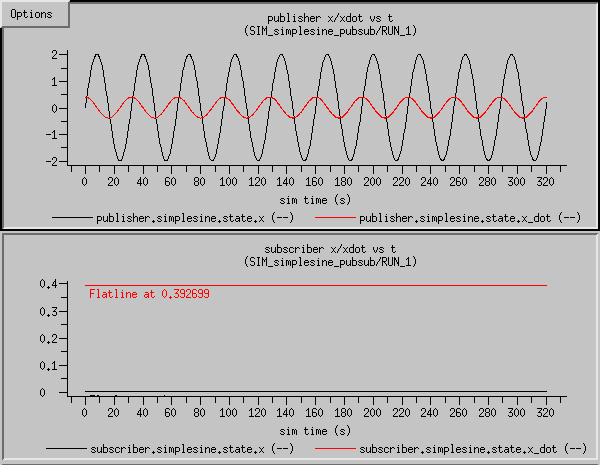
\includegraphics[width=4.5in]{TrickHLAUser-prelim-SIM-pubsub-input-noCopy-noInteg.png}
  \end{center}
\caption{Output from {\tt SIM\_simplesine\_pubsub} using input file {\tt input\_noCopy\_noInteg}}
\label{fig:SIM-pubsub-input-noCopy-noInteg}
\end{figure}


Output from the simulation with {\tt input\_noInteg}
is shown in Figure~\ref{fig:SIM-pubsub-input-noInteg}.
It clearly shows the discrete transfer of data from the publisher to the
subscriber.
Between the data updates, the subscriber state remains constant,
since there is still no numerical intregration on the subscriber side.
This manifests itself in errors which grow significantly until the next
update arrives, at which point the errors reset to zero.

\begin{figure}[b]
  \begin{center}
    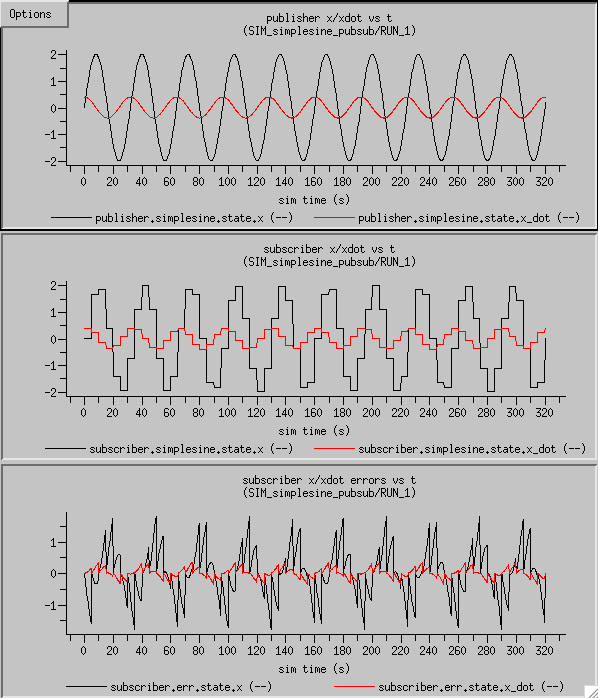
\includegraphics[width=4.5in]{TrickHLAUser-prelim-SIM-pubsub-input-noInteg.png}
  \end{center}
\caption{Output from {\tt SIM\_simplesine\_pubsub} using input file {\tt input\_noInteg}}
\label{fig:SIM-pubsub-input-noInteg}
\end{figure}


Output from the simulation with {\tt input}
is shown in Figure~\ref{fig:SIM-pubsub-input}.
In this case, the subscriber state is ``smoothed'' in between data updates,
since the subscriber numerical integration has been enabled.
Note that there are still errors which grow between updates;
however, in this case the magnitude of those error has diminished by several
orders of magnitude.

\begin{figure}[b]
  \begin{center}
    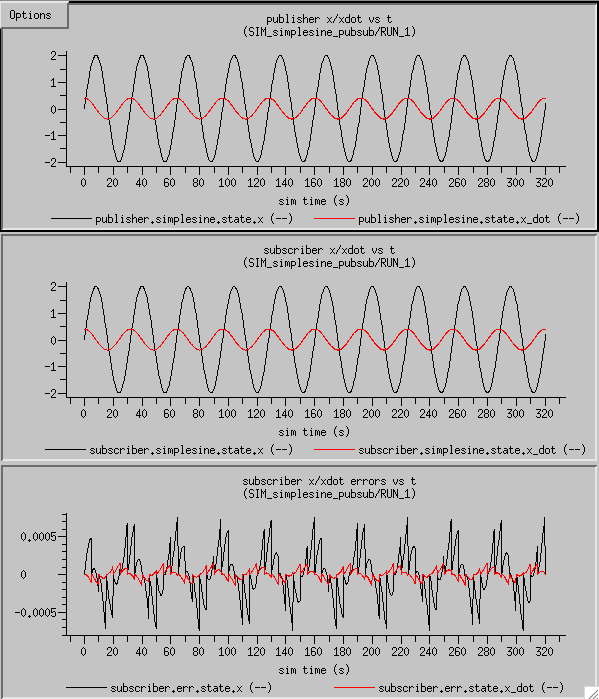
\includegraphics[width=4.5in]{TrickHLAUser-prelim-SIM-pubsub-input.png}
  \end{center}
\caption{Output from {\tt SIM\_simplesine\_pubsub} using input file {\tt input}}
\label{fig:SIM-pubsub-input}
\end{figure}

%
% print the figures before moving to the next chapter
%
\clearpage

\chapter{Joining a Federation}
\label{sec:hla-join}

In this chapter, we present a Trick simulation which uses
\TrickHLA\ to join an HLA federation.\footnote{
  The \TrickHLA\ initialization process is more complex than this
  simulation illustrates.
  The only focus here is on using \TrickHLA\ to enable HLA in a Trick
  simulation.
  The full \TrickHLA\ {\em multi-phase initialzation process} is discussed
  in Section~\ref{sec:hla-init} on page~\pageref{sec:hla-init}.
}
If the specified federation exists,
the simulation joins it.
If the federation does not exist, \TrickHLA\ takes care of creating it.

The simulation
is virtually identical to {\tt SIM\_simplesine\_pubsub} presented in
Section~\ref{sec:simplesine-model}, except that this simulation
joins (or creates) an HLA federation.
In particular, there is no distributed publish/subscribe;
the publisher and subscriber are both resident in this single simulation
process, and they exchange data to each other locally.

The main tasks to HLA-enable an existing Trick simulation are to
insert some ``standard'' \TrickHLA\ {\tt sim\_object}s
into the \sdefine file, and
configure the input file with new \TrickHLA\ parameters.
The following sections illustrate what is involved.

\section{\tt SIM\_simplesine\_hla\_join}
\label{sec:SIM-simplesine-hla-join-sdefine}

The first step in enabling \TrickHLA,
is inserting two new {\tt sim\_object}s into the \sdefine file:
one which contains the main \TrickHLA\ execution
framework (a bunch of jobs that automate the \TrickHLA\ process)
and
one which contains object and jobs related to simulation configuration
and initialization.
The first of these, {\tt THLA}, is shown below
and can be pasted in verbatim.\footnote{
  Some comments have been removed from this object to reduce page space.
}
In most cases, very few modifications to this {\tt sim\_object} should
be necessary.

Examination of the code reveals that \TrickHLA\ is composed of three objects:
the {\em mangager}, the {\em federate}, and the {\em federate ambassador}.
The \TrickHLA\ infrastructure is the base manager and federate jobs
that follow.
In most cases, it is possible to view these objects and their
jobs as black boxes: just paste the object into the \sdefine file.

\begin{lstlisting}[caption={The {\tt THLA sim\_object}},label={list:THLA-sim-object}]
sim_object {
   TrickHLA: TrickHLAFreezeInteractionHandler freeze_ih;
   TrickHLA: TrickHLAFedAmb   federate_amb;
   TrickHLA: TrickHLAFederate federate;
   TrickHLA: TrickHLAManager  manager;
   double checkpoint_time;
   char   checkpoint_label[256];

   // Initialization jobs
   P1 (initialization) TrickHLA: THLA.manager.print_version();
   P1 (initialization) TrickHLA: THLA.federate.fix_FPU_control_word();
   P60 (initialization) TrickHLA: THLA.federate_amb.initialize(
      In TrickHLAFederate * federate = &THLA.federate,
      In TrickHLAManager  * manager  = &THLA.manager );
   P60 (initialization) TrickHLA: THLA.federate.initialize(
      Inout TrickHLAFedAmb * federate_amb = &THLA.federate_amb );
   P60 (initialization) TrickHLA: THLA.manager.initialize(
      In TrickHLAFederate * federate = &THLA.federate );
   P65534 (initialization) TrickHLA: THLA.manager.initialization_complete();
   P65534 (initialization) TrickHLA: THLA.federate.check_pause_at_init( 
      In const double check_pause_delta = THLA_CHECK_PAUSE_DELTA );

   // Checkpoint related jobs
   P1 (checkpoint)          TrickHLA: THLA.federate.setup_checkpoint();
   (freeze)                 TrickHLA: THLA.federate.perform_checkpoint();
   P1 (pre_load_checkpoint) TrickHLA: THLA.federate.setup_restore();
   (freeze)                 TrickHLA: THLA.federate.perform_restore();

   // Freeze jobs
   (freeze)   TrickHLA: THLA.federate.check_freeze();
   (unfreeze) TrickHLA: THLA.federate.exit_freeze();

   // Scheduled jobs
   P1 (THLA_DATA_CYCLE_TIME, environment) TrickHLA: THLA.federate.wait_for_time_advance_grant();
   P1 (THLA_INTERACTION_CYCLE_TIME, environment) TrickHLA: THLA.manager.process_interactions();
   P1 (THLA_DATA_CYCLE_TIME, environment) TrickHLA: THLA.manager.process_deleted_objects();
   P1 (0.0, environment) TrickHLA: THLA.manager.start_federation_save(
      In const char * file_name = THLA.checkpoint_label );
   P1 (0.0, environment) TrickHLA: THLA.manager.start_federation_save_at_sim_time(
      In double freeze_sim_time = THLA.checkpoint_time,
      In const char * file_name = THLA.checkpoint_label );
   P1 (0.0, environment) TrickHLA: THLA.manager.start_federation_save_at_scenario_time(
      In double freeze_scenario_time = THLA.checkpoint_time,
      In const char * file_name = THLA.checkpoint_label );
   P1 (THLA_DATA_CYCLE_TIME, environment) TrickHLA: THLA.manager.receive_cyclic_data();
   P65534 (THLA_DATA_CYCLE_TIME, logging) TrickHLA: THLA.manager.send_cyclic_and_requested_data();
   P65534 (THLA_DATA_CYCLE_TIME, logging) TrickHLA: THLA.manager.process_ownership();
   P65534 (THLA_DATA_CYCLE_TIME, logging) TrickHLA: THLA.federate.time_advance_request();
   P65534 (THLA_DATA_CYCLE_TIME, logging) TrickHLA: THLA.federate.check_freeze_time();
   P65534 (THLA_DATA_CYCLE_TIME, THLA_CHECK_PAUSE_JOB_OFFSET, logging) TrickHLA: THLA.federate.check_pause( 
      In const double check_pause_delta = THLA_CHECK_PAUSE_DELTA );
   P65534 (THLA_DATA_CYCLE_TIME, THLA_CHECK_PAUSE_JOB_OFFSET, logging) TrickHLA: THLA.federate.enter_freeze();

   // Shutdown jobs
   P65534 (shutdown) TrickHLA: THLA.manager.shutdown();
} THLA;
\end{lstlisting}

In addition, the following {\tt THLA\_INIT} object should be put
into the \sdefine file.
The version shown here is sufficient for now.\footnote{
  We will discuss this object in more detail when we address
  \TrickHLA\ multi-phase initialization.
}

\begin{lstlisting}[caption={The {\tt THLA\_INIT sim\_object}},label={list:THLA-INIT-sim-object}]
sim_object {
   // The DSES simulation configuration.
   simconfig: DSESSimConfig  dses_config;

   // Generally, initialization jobs will go here, but not for this example.
   
   // Clear remaining initialization sync-points.
   P100 (initialization) TrickHLA: THLA.manager.clear_init_sync_points();
} THLA_INIT;
\end{lstlisting}

\section{Input Files}

The second step in enabling \TrickHLA\ is to set its parameters in
a Trick input file.
The input file for {\tt SIM\_simplesine\_hla\_join} is shown below.

\begin{lstlisting}[caption={{\tt SIM\_simplesine\_hla\_join} input file},label={list:SIM-simplesine-hla-join-input}]
#include "S_properties"
#include "S_default.dat"
#include "Log_data/states.d"
#include "Modified_data/realtime.d"
#include "Modified_data/publisher.d"
#include "Modified_data/subscriber.d"

stop =32.5;

//
// Basic RTI/federation connection info
//

// Configure the CRC for the Pitch RTI.
THLA.federate.local_settings = "crcHost = localhost\n crcPort = 8989";

THLA.federate.name            = "pubsub_join";
THLA.federate.FOM_modules     = "FOM.xml";
THLA.federate.federation_name = "simplesine";

THLA.federate.lookahead_time   = THLA_DATA_CYCLE_TIME;
THLA.federate.time_regulating  = true;
THLA.federate.time_constrained = true;
THLA.federate.multiphase_init_sync_points = "Phase1, Phase2";

THLA.federate.enable_known_feds      = true;
THLA.federate.known_feds_count       = 1;
THLA.federate.known_feds             = alloc(THLA.federate.known_feds_count);
THLA.federate.known_feds[0].name     = "pubsub_join";
THLA.federate.known_feds[0].required = true;

// TrickHLA debug messages.
THLA.manager.debug_handler.debug_level = THLA_LEVEL2_TRACE;

//
// SimConfig initialization
//

// DSES simulation configuration.
THLA_INIT.dses_config.owner              = "pubsub_join";
THLA_INIT.dses_config.run_duration       = 15.0;
THLA_INIT.dses_config.num_federates      = 1;
THLA_INIT.dses_config.required_federates = "pubsub_join";
THLA_INIT.dses_config.start_year         = 2007;
THLA_INIT.dses_config.start_seconds      = 0;
THLA_INIT.dses_config.scenario           = "Nominal";
THLA_INIT.dses_config.mode               = "Unknown";

// Simulation Configuration for DSES Multi-phase Initialization.
THLA.manager.sim_config.FOM_name         = "SimulationConfiguration";
THLA.manager.sim_config.name             = "SimConfig";
THLA.manager.sim_config.packing          = &THLA_INIT.dses_config;
THLA.manager.sim_config.attr_count       = 8;
THLA.manager.sim_config.attributes       = alloc(THLA.manager.sim_config.attr_count);

THLA.manager.sim_config.attributes[0].FOM_name     = "owner";
THLA.manager.sim_config.attributes[0].trick_name   = "THLA_INIT.dses_config.owner";
THLA.manager.sim_config.attributes[0].publish      = true;
THLA.manager.sim_config.attributes[0].subscribe    = true;
THLA.manager.sim_config.attributes[0].rti_encoding = THLA_UNICODE_STRING;

THLA.manager.sim_config.attributes[1].FOM_name     = "run_duration";
THLA.manager.sim_config.attributes[1].trick_name   = "THLA_INIT.dses_config.run_duration_microsec";
THLA.manager.sim_config.attributes[1].publish      = true;
THLA.manager.sim_config.attributes[1].subscribe    = true;
THLA.manager.sim_config.attributes[1].rti_encoding = THLA_LITTLE_ENDIAN;

THLA.manager.sim_config.attributes[2].FOM_name     = "number_of_federates";
THLA.manager.sim_config.attributes[2].trick_name   = "THLA_INIT.dses_config.num_federates";
THLA.manager.sim_config.attributes[2].publish      = true;
THLA.manager.sim_config.attributes[2].subscribe    = true;
THLA.manager.sim_config.attributes[2].rti_encoding = THLA_LITTLE_ENDIAN;

THLA.manager.sim_config.attributes[3].FOM_name     = "required_federates";
THLA.manager.sim_config.attributes[3].trick_name   = "THLA_INIT.dses_config.required_federates";
THLA.manager.sim_config.attributes[3].publish      = true;
THLA.manager.sim_config.attributes[3].subscribe    = true;
THLA.manager.sim_config.attributes[3].rti_encoding = THLA_UNICODE_STRING;

THLA.manager.sim_config.attributes[4].FOM_name     = "start_year";
THLA.manager.sim_config.attributes[4].trick_name   = "THLA_INIT.dses_config.start_year";
THLA.manager.sim_config.attributes[4].publish      = true;
THLA.manager.sim_config.attributes[4].subscribe    = true;
THLA.manager.sim_config.attributes[4].rti_encoding = THLA_LITTLE_ENDIAN;

THLA.manager.sim_config.attributes[5].FOM_name     = "start_seconds";
THLA.manager.sim_config.attributes[5].trick_name   = "THLA_INIT.dses_config.start_seconds";
THLA.manager.sim_config.attributes[5].publish      = true;
THLA.manager.sim_config.attributes[5].subscribe    = true;
THLA.manager.sim_config.attributes[5].rti_encoding = THLA_LITTLE_ENDIAN;

THLA.manager.sim_config.attributes[6].FOM_name     = "scenario";
THLA.manager.sim_config.attributes[6].trick_name   = "THLA_INIT.dses_config.scenario";
THLA.manager.sim_config.attributes[6].publish      = true;
THLA.manager.sim_config.attributes[6].subscribe    = true;
THLA.manager.sim_config.attributes[6].rti_encoding = THLA_UNICODE_STRING;

THLA.manager.sim_config.attributes[7].FOM_name     = "mode";
THLA.manager.sim_config.attributes[7].trick_name   = "THLA_INIT.dses_config.mode";
THLA.manager.sim_config.attributes[7].publish      = true;
THLA.manager.sim_config.attributes[7].subscribe    = true;
THLA.manager.sim_config.attributes[7].rti_encoding = THLA_UNICODE_STRING;

//
// Object info
//
THLA.manager.obj_count = 0;

//
// Interaction info
//
THLA.manager.inter_count = 0;
\end{lstlisting}

Lines 2-8 are identical to the input file for {\tt SIM\_simplesine\_pubsub}.
Everything else is new.

Lines 16-18 initialize the federation, supplying values for this federate's
name, the name of the federation to join, the host/port information for the
HLA RTI,\footnote{
  The standard port number is 8989.
  During development the host is often set to localhost, but in general
  the RTI will be running on some agreed location on the network.
}
and the name of the FOM file (located in the same directory as the
\sdefine file).

Lines 20-22 are related to HLA time management: the {\em lookahead time},
and two flags indicating whether the simulation is {\em time regulating}
and {\em time constrained}.
All the examples in this document use a lookahead of just under 1sec
and are both time constrained and time regulating.

Lines 24-28 itemizes a list of {\em known federates}.
This is the \TrickHLA\ mechanism for ensuring that federates wait for
everyone to join before proceeding.
In this example, there is only a single federate ({\tt pubsub\_join}),
but in cases where there are several, the array would be allocated
to hold them all, specifying the name of each and whether they are
required to be present before the others may proceed.

Line 31 is setting the global debug level flags and lead to gradually more or less verbose output.

Lines 38-45 initialize the federation's {\tt SimulationConfiguration} object.
There is one (and only one) of these instances for all the
federates in the federation, but each one (if it uses \TrickHLA)
will nevertheless set these values.
The \TrickHLA\ infrastructure ensures that even though many federates
attempt to publish the object, it only gets created by one of them.
One point worth noting: the value on line 39 for the
{\tt .run\_duration} parameter ensures that the simulation does not run
longer than the specified duration, even if that duration is less than
the value specified with the {\tt STOP} directive (on line 7).

Lines 48-101 are also related to the {\tt SimulationConfiguration} object
as well as multi-phase initialization.
(We do not discuss multi-phase initialization in this example.)

Finally, lines 106 and 111 specify that this simulation has no objects
to publish or subscribe and no interactions to send or receive.
Subsequent examples will elaborate on the \TrickHLA\ publish/subscribe
mechanisms.

\section{Output}

The relevant output for this simulation is the output stream from the
running simulation, which (among other things) verifies that the simulation
did indeed create and join an HLA federation.
An abbreviated version of the output is shown below.

\begin{lstlisting}[caption={{\tt SIM\_simplesine\_hla\_join} output},label={list:SIM-simplesine-hla-join-output}]
...
| |wormhole|1|0.00|2007/07/25,17:59:09| TrickHLAFedAmb::initialize()
| |wormhole|1|0.00|2007/07/25,17:59:09| TrickHLAFederate::initialize()
| |wormhole|1|0.00|2007/07/25,17:59:09| TrickHLAManager::initialize()
...
| |wormhole|1|0.00|2007/07/25,17:59:10|
 TRIVIAL: Trick Federation "simplesine": CREATING FEDERATION EXECUTION
| |wormhole|1|0.00|2007/07/25,17:59:10|
 ADVISORY: Trick Federation "simplesine": SUCCESSFULLY CREATED FEDERATION EXECUTION
| |wormhole|1|0.00|2007/07/25,17:59:10|
 TRIVIAL: Trick Federation "simplesine": JOINING FEDERATION EXECUTION
| |wormhole|1|0.00|2007/07/25,17:59:10|
 ADVISORY: Trick Federation "simplesine": JOINED FEDERATION EXECUTION
Federate Handle = 2
...
| |wormhole|1|0.00|2007/07/25,17:59:10| TrickHLAFederate::wait_for_required_federates_to_join()
WAITING FOR 1 REQUIRED FEDERATES:
    1: Waiting for Federate 'pubsub_join'
...
| |wormhole|1|0.00|2007/07/25,17:59:10| TrickHLAFederate::wait_for_required_federates_to_join()
WAITING FOR 1 REQUIRED FEDERATES:
    1: Found required Federate 'pubsub_join'
...
| |wormhole|1|0.00|2007/07/25,17:59:10| TrickHLAManager::initialization_complete()
        Simulation has started and is now running...
...
Federate "pubsub_join" Time granted to: 1
...
Federate "pubsub_join" Time granted to: 16
...
 TRIVIAL: Trick Federation "simplesine": RESIGNING FROM FEDERATION
...
 ADVISORY: Trick Federation "simplesine": RESIGNED FROM FEDERATION
...
Federation destroyed
...
SIMULATION TERMINATED IN
  PROCESS: 1
  JOB/ROUTINE: 11/sim_services/mains/master.c
DIAGNOSTIC:
Simulation reached input termination time.

LAST JOB CALLED: THLA.THLA.federate.time_advance_request()
              TOTAL OVERRUNS:            0
PERCENTAGE REALTIME OVERRUNS:        0.000%


       SIMULATION START TIME:        0.000
        SIMULATION STOP TIME:       15.000
     SIMULATION ELAPSED TIME:       15.000
         ACTUAL ELAPSED TIME:       15.000
        ACTUAL CPU TIME USED:        0.040
    SIMULATION / ACTUAL TIME:        1.000
       SIMULATION / CPU TIME:      375.056
  ACTUAL INITIALIZATION TIME:        0.000
     INITIALIZATION CPU TIME:        0.719
*** DYNAMIC MEMORY USAGE ***
     CURRENT ALLOCATION SIZE:  1569508
       NUM OF CURRENT ALLOCS:      483
         MAX ALLOCATION SIZE:  1569508
           MAX NUM OF ALLOCS:      483
       TOTAL ALLOCATION SIZE:  1794096
         TOTAL NUM OF ALLOCS:     3301
\end{lstlisting}

Lines 1-14 show the simulation running through its startup process,
initializing the \TrickHLA\ objects which in turn create and join
the HLA federation names {\em simplesine}.

Lines 16-25 show the simulation waiting for all the required federates to join,
which in this case is just this simulation.

Lines 27-29 show the beginning and end of the time grants issues by HLA,
starting at $t=1$ and going thru the end of the simulation duration,
as $t$ extended past the specified limit of 15.

Lines 31-35 show the simulation resigning from the federation and
destroying it (since no federates remain).

The remaining lines are standard Trick output generated at the end of a run.
Note that in spite of the fact that the input file specified
{\tt stop = 32.5} as shown on line 7 of the input file
(Listing~\ref{list:SIM-simplesine-hla-join-input} on page~\pageref{list:SIM-simplesine-hla-join-input}),
the simulation actually terminated earlier due to the
simulation configuration {\tt .run\_duration = 15.0} as specified in
the input file.

\chapter{Publishing and Subscribing}
\label{sec:hla-pubsub}

In this chapter,
we present two Trick simulations:
one that publishes sine wave data via HLA
and one that subscribes.
Together, these represent a distributed, HLA
version of the simple publish/subscribe simulation that was discussed
in Section~\ref{sec:simplesine-pubsub-sdefine} on page~\pageref{sec:simplesine-pubsub-sdefine}.

% ------------------------------------------------------------------------
\section{{\tt SIM\_simplesine\_hla\_pub}}
This section discusses the \sdefine file for a publisher.
The file is very similar to that discussed in
Section~\ref{sec:SIM-simplesine-hla-join-sdefine}
on page~\pageref{sec:SIM-simplesine-hla-join-sdefine},
except that there is no subscriber:
the subscriber {\tt sim\_object} is gone,
the publisher no longer has a job to copy data to the subscriber, and
there is no Trick {\tt integrate} directive for the
subscriber's numerical integraion.

An abbreviated version file is shown below.
(The full {\tt THLA} and {\tt THLA\_INIT} sim objects
are identical to those in the {\tt SIM\_simplesine\_hla\_join} file.)

\begin{lstlisting}[caption={{\tt SIM\_simplesine\_hla\_pub} \sdefine},label={list:SIM-simplesine-hla-pub-sdefine}]
#include "S_properties"

#define PROPAGATE_TIMESTEP 0.25

sim_object
{
  sim_services/include: EXECUTIVE exec (sim_services/include/executive.d) ;

  (automatic) sim_services/input_processor:
    input_processor( INPUT_PROCESSOR* IP = &sys.exec.ip ) ;
} sys ;

sim_object
{
  simplesine: simplesine_T simplesine (simplesine/data/simplesine.d);

  (initialization) simplesine:
    simplesine_calc(
      simplesine_T* P = &publisher.simplesine,
      double t = sys.exec.out.time );
  (PROPAGATE_TIMESTEP, scheduled) simplesine:
    simplesine_calc(
      simplesine_T* P = &publisher.simplesine,
      double t = sys.exec.out.time );
} publisher ;

#include "S_modules/THLA.sm"

sim_object {
  ...
} THLA_INIT;
\end{lstlisting}

% ------------------------------------------------------------------------
\section{{\tt SIM\_simplesine\_hla\_sub}}
This section discusses the \sdefine file for a \TrickHLA\ publisher.
Like the publisher above, this file is similar to the \sdefine file for
the non-HLA publisher/subscriber
in Section~\ref{sec:simplesine-pubsub-sdefine} on page~\pageref{sec:simplesine-pubsub-sdefine},
except that this file has no publisher object.
An abbreviated version of the subscriber's \sdefine is shown below.

\begin{lstlisting}[caption={{\tt SIM\_simplesine\_hla\_sub} \sdefine},label={list:SIM-simplesine-hla-sub-sdefine}]
#include "S_properties"

#define PROPAGATE_TIMESTEP 0.25
#define COPY_TIMESTEP 5.0

sim_object
{
  sim_services/include: EXECUTIVE exec (sim_services/include/executive.d) ;

  (automatic) sim_services/input_processor:
    input_processor( INPUT_PROCESSOR* IP = &sys.exec.ip ) ;
} sys ;


sim_object
{
  sim_services/include: INTEGRATOR integ (simplesine/data/integ.d);
  simplesine: simplesine_T simplesine;
  simplesine: simplesine_T err;

  (initialization) simplesine:
    simplesine_calc(
      simplesine_T* P = &subscriber.simplesine,
      double t = sys.exec.out.time );

  (derivative) simplesine:
    simplesine_deriv( simplesine_T* p = &subscriber.simplesine );

  (integration) simplesine:
    simplesine_integ(
      INTEGRATOR* I = &subscriber.integ,
      simplesine_T* p = &subscriber.simplesine );

  (PROPAGATE_TIMESTEP, scheduled) simplesine:
    simplesine_calcError(
      double t = sys.exec.out.time,
      simplesine_T* s = &subscriber.simplesine,
      simplesine_state_T* err = &subscriber.err.state );

} subscriber ;

integrate (PROPAGATE_TIMESTEP) subscriber;

#include "S_modules/THLA.sm"

sim_object {
  ...
} THLA_INIT;
\end{lstlisting}

% ------------------------------------------------------------------------
\section{Publisher input file}

The publisher's input file is shown below.
It is very similar to the input file used for the join example
in the previous chapter.
The differences are
\begin{itemize}
\item{
  this federate has a different name ({\em publisher}),
}
\item{
  the simulation waits for the {\em subscriber} federate to
  join the federation, and
}
\item{
  one object class is defined to the data which this simulation
  publishes.
}
\end{itemize}

The last difference is the most significant.
To add object classes to a simulation, all that is required is that
you declare them in the input file.\footnote{
  Of course, the object class in question must already be declared in
  the FOM.
}
For this simulation,
the relevant additions to the input file are shown below.

\begin{lstlisting}[caption={{\tt SIM\_simplesine\_hla\_pub} input file},label={list:hla-pub-input}]
// This federate has one object which is publishes.
THLA.manager.obj_count = 1;
THLA.manager.objects   = alloc(THLA.manager.obj_count);

// Configure the object this federate owns and will publish.
THLA.manager.objects[0].FOM_name            = "SimplesineStateAndParameters";
THLA.manager.objects[0].name                = "simplesineStateAndParameters";
THLA.manager.objects[0].create_HLA_instance = true;
THLA.manager.objects[0].attr_count          = 6;
THLA.manager.objects[0].attributes          = alloc(THLA.manager.objects[0].attr_count);

THLA.manager.objects[0].attributes[0].FOM_name      = "Time";
THLA.manager.objects[0].attributes[0].trick_name    = "sys.exec.out.time";
THLA.manager.objects[0].attributes[0].config        = THLA_CYCLIC;
THLA.manager.objects[0].attributes[0].publish       = true;
THLA.manager.objects[0].attributes[0].locally_owned = true;
THLA.manager.objects[0].attributes[0].rti_encoding  = THLA_LITTLE_ENDIAN;

THLA.manager.objects[0].attributes[1].FOM_name      = "Value";
THLA.manager.objects[0].attributes[1].trick_name    = "publisher.simplesine.state.x";
THLA.manager.objects[0].attributes[1].config        = THLA_INITIALIZE + THLA_CYCLIC;
THLA.manager.objects[0].attributes[1].publish       = true;
THLA.manager.objects[0].attributes[1].locally_owned = true;
THLA.manager.objects[0].attributes[1].rti_encoding  = THLA_LITTLE_ENDIAN;

THLA.manager.objects[0].attributes[2].FOM_name      = "dvdt";
THLA.manager.objects[0].attributes[2].trick_name    = "publisher.simplesine.state.x_dot";
THLA.manager.objects[0].attributes[2].config        = THLA_CYCLIC;
THLA.manager.objects[0].attributes[2].publish       = true;
THLA.manager.objects[0].attributes[2].locally_owned = true;
THLA.manager.objects[0].attributes[2].rti_encoding  = THLA_LITTLE_ENDIAN;

THLA.manager.objects[0].attributes[3].FOM_name      = "Phase";
THLA.manager.objects[0].attributes[3].trick_name    = "publisher.simplesine.params.phi";
THLA.manager.objects[0].attributes[3].config        = THLA_CYCLIC;
THLA.manager.objects[0].attributes[3].publish       = true;
THLA.manager.objects[0].attributes[3].locally_owned = true;
THLA.manager.objects[0].attributes[3].rti_encoding  = THLA_LITTLE_ENDIAN;

THLA.manager.objects[0].attributes[4].FOM_name      = "Frequency";
THLA.manager.objects[0].attributes[4].trick_name    = "publisher.simplesine.params.w";
THLA.manager.objects[0].attributes[4].config        = THLA_CYCLIC;
THLA.manager.objects[0].attributes[4].publish       = true;
THLA.manager.objects[0].attributes[4].locally_owned = true;
THLA.manager.objects[0].attributes[4].rti_encoding  = THLA_LITTLE_ENDIAN;

THLA.manager.objects[0].attributes[5].FOM_name      = "Amplitude";
THLA.manager.objects[0].attributes[5].trick_name    = "publisher.simplesine.params.A";
THLA.manager.objects[0].attributes[5].config        = THLA_CYCLIC;
THLA.manager.objects[0].attributes[5].publish       = true;
THLA.manager.objects[0].attributes[5].locally_owned = true;
THLA.manager.objects[0].attributes[5].rti_encoding  = THLA_LITTLE_ENDIAN;
\end{lstlisting}

This set of inputs tells \TrickHLA\ that the simulation will be publishing
an object with six attributes.

Lines 2-3 indicate that only a single object is involved.

Lines 6-7 specify that the object instance will be named
{\tt simplesineStateAndParameters} and that it is an instance of the class
{\tt SimplesineStateAndParameters} (which must be defined in the FOM).

Line 8 indicates that the instance will be owned by this simulation.

Lines 10-11 specify that the simulation is interested in six attributes
of the instance -- in this case all of them.

The subsequent lines specify per-attribute settings:
the name of the attribute as specified in the class definition in the FOM,
the name of the Trick variable associated with the attribute,
whether the attribute is owned locally,
whether this simulation intends to publish values for the attribute,
and how the data is to be encoded when it is sent over the network.
Notice that the trick variables specified are {\simplesine} parameters
and state located in the publisher object.

By associating Trick variables with attributes in this fashion,
whenever the \TrickHLA\ infrastructure sends out updates
(as defined in the {\tt THLA} object in the \sdefine file),
the current value of the corresponding Trick variable will be used.
Simulation developers need do nothing explicit to send data --
the \TrickHLA\ infrastructure handles that task.

% ------------------------------------------------------------------------
\section{Subscriber input file}

Like the publisher, the subscriber's input file is similar to the join example
in the previous chapter.
The differences are
\begin{itemize}
\item{
  this federate has a different name ({\em subscriber}).
}
\item{
  the simulation waits for the {\em publisher} federate to join
  the federation, and
}
\item{
  an object class is defined for the data to which this federate
  subscribes.
}
\end{itemize}

Indeed, the subscriber inputs are very similar to the publisher inputs above
with the exception that
local ownership is turned off,
publishing is turned off, and
subscribing is turned on.

The relevant object declarations are shown below.

\begin{lstlisting}[caption={{\tt SIM\_simplesine\_hla\_sub} input file},label={list:hla-sub-input}]
// This federate has only one object, and it subscribes to it.
THLA.manager.obj_count = 1;
THLA.manager.objects   = alloc(THLA.manager.obj_count);

// objects subscribed to
THLA.manager.objects[0].FOM_name            = "SimplesineStateAndParameters";
THLA.manager.objects[0].name                = "simplesineStateAndParameters";
THLA.manager.objects[0].create_HLA_instance = false;
THLA.manager.objects[0].attr_count          = 6;
THLA.manager.objects[0].attributes          = alloc(THLA.manager.objects[0].attr_count);

THLA.manager.objects[0].attributes[0].FOM_name      = "Time";
THLA.manager.objects[0].attributes[0].trick_name    = "sys.exec.out.time";
THLA.manager.objects[0].attributes[0].config        = THLA_CYCLIC;
THLA.manager.objects[0].attributes[0].publish       = false;
THLA.manager.objects[0].attributes[0].subscribe     = true;
THLA.manager.objects[0].attributes[0].locally_owned = false;
THLA.manager.objects[0].attributes[0].rti_encoding  = THLA_LITTLE_ENDIAN;

THLA.manager.objects[0].attributes[1].FOM_name      = "Value";
THLA.manager.objects[0].attributes[1].trick_name    = "subscriber.simplesine.state.x";
THLA.manager.objects[0].attributes[1].config        = THLA_INITIALIZE + THLA_CYCLIC;
THLA.manager.objects[0].attributes[1].publish       = false;
THLA.manager.objects[0].attributes[1].subscribe     = true;
THLA.manager.objects[0].attributes[1].locally_owned = false;
THLA.manager.objects[0].attributes[1].rti_encoding  = THLA_LITTLE_ENDIAN;

THLA.manager.objects[0].attributes[2].FOM_name      = "dvdt";
THLA.manager.objects[0].attributes[2].trick_name    = "subscriber.simplesine.state.x_dot";
THLA.manager.objects[0].attributes[2].config        = THLA_CYCLIC;
THLA.manager.objects[0].attributes[2].publish       = false;
THLA.manager.objects[0].attributes[2].subscribe     = true;
THLA.manager.objects[0].attributes[2].locally_owned = false;
THLA.manager.objects[0].attributes[2].rti_encoding  = THLA_LITTLE_ENDIAN;

THLA.manager.objects[0].attributes[3].FOM_name      = "Phase";
THLA.manager.objects[0].attributes[3].trick_name    = "subscriber.simplesine.params.phi";
THLA.manager.objects[0].attributes[3].config        = THLA_CYCLIC;
THLA.manager.objects[0].attributes[3].publish       = false;
THLA.manager.objects[0].attributes[3].subscribe     = true;
THLA.manager.objects[0].attributes[3].locally_owned = false;
THLA.manager.objects[0].attributes[3].rti_encoding  = THLA_LITTLE_ENDIAN;

THLA.manager.objects[0].attributes[4].FOM_name      = "Frequency";
THLA.manager.objects[0].attributes[4].trick_name    = "subscriber.simplesine.params.w";
THLA.manager.objects[0].attributes[4].config        = THLA_CYCLIC;
THLA.manager.objects[0].attributes[4].publish       = false;
THLA.manager.objects[0].attributes[4].subscribe     = true;
THLA.manager.objects[0].attributes[4].locally_owned = false;
THLA.manager.objects[0].attributes[4].rti_encoding  = THLA_LITTLE_ENDIAN;

THLA.manager.objects[0].attributes[5].FOM_name      = "Amplitude";
THLA.manager.objects[0].attributes[5].trick_name    = "subscriber.simplesine.params.A";
THLA.manager.objects[0].attributes[5].config        = THLA_CYCLIC;
THLA.manager.objects[0].attributes[5].publish       = false;
THLA.manager.objects[0].attributes[5].subscribe     = true;
THLA.manager.objects[0].attributes[5].locally_owned = false;
THLA.manager.objects[0].attributes[5].rti_encoding  = THLA_LITTLE_ENDIAN;
\end{lstlisting}


\section{Output}

Together, these two simulations do in a distributed fashion what
the single simulation did in Chapter~\ref{sec:simplesine-sim}.
The publisher generates sine wave data and periodically sends updates
to the subscriber.
The subscriber receives the periodic updates and extrapolates the state
until the next update arrives.

Figure~\ref{fig:hla-pub-output} shows the sine wave as generated on
the publisher.
Figure~\ref{fig:hla-sub-noInteg-output} shows the sine wave as received by
the subscriber with numerical integration disabled to emphasize the
time of arrival of the data.
Figure~\ref{fig:hla-sub-output} shows the sine wave generated by the
subscriber based on data received from the publisher with subscriber-side
numerical integration between updates.

Close inspection of the publisher and subscriber plots reveals that
they are slightly out of phase, hence the relatively large error
in the third plot.
This phase lag is due to HLA time management {\em lookahead},
which is 1.0sec in this case.
Indeed, this effect can be seen clearly at $t=1$, since up until that
point the subscriber was integrating based solely on initial conditions
(not based on any data received from the publisher),
but at $t=1$, the first data arrives from the publisher but it is
approximately 1sec late, resulting in a discontinuity in the data.
This lookahead-induced effect can be compensated using \TrickHLA\ features
discussed in Chapter~\ref{sec:hla-lag}.

\begin{figure}[b]
  \begin{center}
    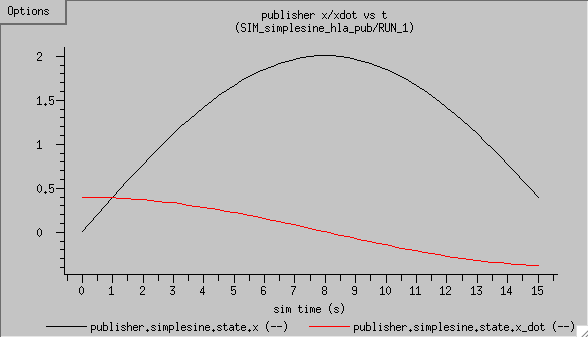
\includegraphics[width=4.5in]{TrickHLAUser-SIM-hla-pub.png}
  \end{center}
\caption{Output from {\tt SIM\_simplesine\_hla\_pub}}
\label{fig:hla-pub-output}
\end{figure}

\begin{figure}[b]
  \begin{center}
    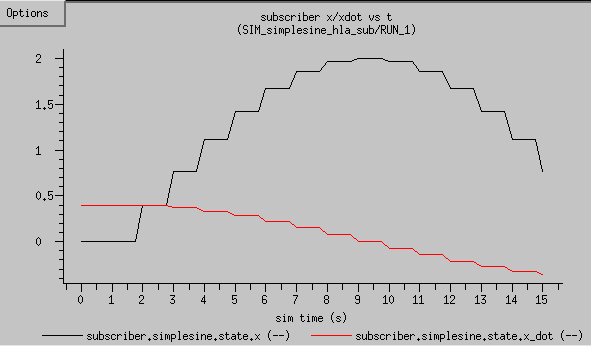
\includegraphics[width=4.5in]{TrickHLAUser-SIM-hla-sub-noInteg.png}
  \end{center}
\caption{Output from {\tt SIM\_simplesine\_hla\_sub} (no integration)}
\label{fig:hla-sub-noInteg-output}
\end{figure}

\begin{figure}[b]
  \begin{center}
    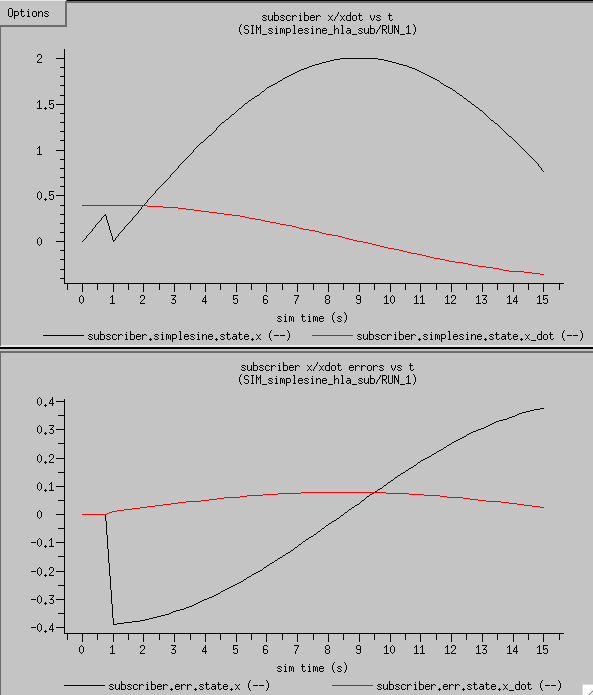
\includegraphics[width=4.5in]{TrickHLAUser-SIM-hla-sub.png}
  \end{center}
\caption{Output from {\tt SIM\_simplesine\_hla\_pub}}
\label{fig:hla-sub-output}
\end{figure}



\chapter{Lag Compensation}
\label{sec:hla-lag}

In this chapter,
we present simulations which compensate for time lags introduced due to
HLA time management.
The lags appear when published data are sent from one federate to
its subscribers, and
it becomes particularly noticeable when data ownership is transferred
between federates.

There are two \TrickHLA\ mechanisms which allow simulation developers
to compensate for HLA-introduced lag:
publisher-side and subscriber-side compensation.

% -------------------------------------------------------------------------
\section{What is a Lag Compensator?}

% -----------------------------------
\subsection{The class {\tt TrickHLALagCompensation}}

\TrickHLA\ defines a C++ class which may be subclassed by simulation
developers in order to implement either kind of lag compensation.
The class header is shown below.

\begin{lstlisting}[caption={The {\tt TrickHLALagCompensation} class},label={list:TrickHLALagCompensation}]
class TrickHLALagCompensation
{
   friend class InputProcessor;
   friend void init_attrTrickHLALagCompensation();

  public:
   TrickHLALagCompensation() {};           // default constructor
   virtual ~TrickHLALagCompensation() {};  // destructor

   virtual void send_lag_compensation();   // RETURN: -- None.

   virtual void receive_lag_compensation() // RETURN: -- None.
};
\end{lstlisting}

To use this class,
simulation developers subclass it, overriding the relevant send/receive methods.
The \TrickHLA\ infrastructure automatically invokes those methods
for publishers and subscribers at the appropriate time.

Developers only need to be concerned with the algorithm defined in these
methods; the logistics of invoking them at the appropriate time is taken
handled by \TrickHLA.
The following subsections illustrate how this is done in the \simplesine
model.

% -----------------------------------
\subsection{Lag compensation in \simplesine}
% -------------
\subsubsection{\tt simplesine\_compensate()}

The \simplesine model includes a {\tt simplesine\_compensate()} function
which does most of the lag compensation work.
It is based on the equations~\ref{eq:analytic-equations}.
Using those equations, the state at time $t + \Delta t$ can be written as
\begin{subequations}
\label{eq:analytic-compensation-equations}
\begin{align}
x(t + \Delta t)       &= A        \sin {(\omega (t + \Delta t) + \phi)}, \\
\dot{x}(t + \Delta t) &= A \omega \cos {(\omega (t + \Delta t) + \phi)}.
\end{align}
\end{subequations}

With a bit of trignometry and rearranging, the compensated state at time
$t + \Delta t$ can be written in terms of the uncompensated state at time $t$
as follows.
\begin{subequations}
\label{eq:analytic-compensation-equations-2}
\begin{align}
x(t + \Delta t)
  &=
    x(t)       \cos {\omega \Delta t}
    +
    \frac{\dot{x}(t)}{\omega} \sin { \omega \Delta t}
  \\
\dot{x}(t + \Delta t)
  &=
    \dot{x}(t) \cos {\omega \Delta t}
    -
    x(t) \omega \sin { \omega \Delta t}
\end{align}
\end{subequations}

The compensate function is shown below.
It takes an uncompensated state and $\Delta t$ as inputs
and calculates the corresonded compensated state at time $t + \Delta t$.

\begin{lstlisting}[caption={The {\tt simplesine\_compensate} function},label={list:simplesine-compensate}]
void simplesine_compensate(
  simplesine_params_T* paramsP,
  simplesine_state_T* uncompensated_stateP,
  simplesine_state_T* compensated_stateP,
  double dt )
{
  const double w = paramsP->w;
  const double wdt = w * dt;
  const double sinwdt = sin( wdt );
  const double coswdt = cos( wdt );

  const double x     = uncompensated_stateP->x;
  const double x_dot = uncompensated_stateP->x_dot;

  // Calculate the compensated state.
  const double x_compensated     = x     * coswdt  +  x_dot * sinwdt / w ;
  const double x_dot_compensated = x_dot * coswdt  -  x     * sinwdt * w;

  // Save the compenstated state.
  compensated_stateP->x     = x_compensated;
  compensated_stateP->x_dot = x_dot_compensated;
}
\end{lstlisting}

% -------------
\subsubsection{\tt simplesine\_LagCompensation}

The simplesine subsclass of {\tt TrickHLALagCompensation} is shown below.
It relies on the {\tt simple\-sine\-\_comp\-ensate()} function to do the real work, transforming the uncompensated state pointed to by
{\tt uncompensated\_stateP}
into a transformed state pointed to by
{\tt compensated\_stateP}.
These two pointers are initialized by the {\tt initialize()} method,
which is unique to this class (i.e., not part of the interface defined by the
{\tt TrickHLALagCompensation} class).

\begin{lstlisting}[caption={The {\tt simplesine\_LagCompensation} class header},label={list:simplesine-LagCompensation-header}]
#include "simplesine.h"
#include "TrickHLA/include/TrickHLALagCompensation.hh"

class simplesine_LagCompensator : public TrickHLALagCompensation
{
  friend class InputProcessor;
  friend void init_attrsimplesine_LagCompensator();

  public:
   simplesine_LagCompensator();
   virtual ~simplesine_LagCompensator();

   int initialize( simplesine_T* sim_dataP, simplesine_T* lag_comp_dataP );
   virtual void send_lag_compensation();
   virtual void receive_lag_compensation();

  private:
    simplesine_T* uncompensated_stateP;
    simplesine_T* compensated_stateP;
};
\end{lstlisting}

\begin{lstlisting}[caption={The {\tt simplesine\_LagCompensation} class methods},label={list:simplesine-LagCompensation-methods}]
/********************************* TRICK HEADER *******************************
PURPOSE: (This class provides lag compensation.)
LIBRARY DEPENDENCY: ((simplesine_compensate.o))
*******************************************************************************/
// System include files.
#include <math.h>
#include <stdlib.h>
#include <iostream>
#include <string>

using namespace std;

#include "sim_services/include/exec_proto.h"
#include "trick_utils/math/include/trick_math.h"

#include "../include/simplesine_proto.h"
#include "../include/simplesine_LagCompensator.hh"

/* ---------------------------------------------------------------------------
PURPOSE: (Default constructor for the sine wave lag compensation.)
------------------------------------------------------------------------------*/
simplesine_LagCompensator::simplesine_LagCompensator() // RETURN: -- None.
{ }

/* ---------------------------------------------------------------------------
PURPOSE: (Frees memory allocated.)
------------------------------------------------------------------------------*/
simplesine_LagCompensator::~simplesine_LagCompensator() // RETURN: -- None.
{ }

/* ---------------------------------------------------------------------------
PURPOSE: (Initializes the Sine Lag Compensation.)
------------------------------------------------------------------------------*/
int simplesine_LagCompensator::initialize( // RETURN: -- Always returns zero.
      simplesine_T * uncompensated_stateP, // IN:     -- Simulation data.
      simplesine_T * compensated_stateP )  // IN:     -- Lag Compensation data.
{
   this->uncompensated_stateP = uncompensated_stateP;
   this->compensated_stateP = compensated_stateP;
   return( 0 );
}

/* ---------------------------------------------------------------------------
PURPOSE: (Send-side lag-compensation where we propagate the sine wave
  state head by dt to predict the value at the next data cycle.)
------------------------------------------------------------------------------*/
void simplesine_LagCompensator::send_lag_compensation() // RETURN: -- None.
{
   double dt = get_fed_lookahead().getDoubleTime();

   simplesine_compensate( &(uncompensated_stateP->params),
                          &(uncompensated_stateP->state),
                          &(compensated_stateP->state),
                          dt );
}

/* ---------------------------------------------------------------------------
PURPOSE: (Receiveside lag-compensation where we propagate the sine wave
  state ahead by dt to predict the value at the next data cycle.)
------------------------------------------------------------------------------*/
void simplesine_LagCompensator::receive_lag_compensation() // RETURN: -- None.
{
   double dt = get_fed_lookahead().getDoubleTime();

   simplesine_compensate( &(uncompensated_stateP->params),
                          &(uncompensated_stateP->state),
                          &(compensated_stateP->state),
                          dt );
}
\end{lstlisting}


% -------------------------------------------------------------------------
\section{Publisher-resident Compensation}

This approach to lag compensation is handled by the publisher of data before
it is sent out via HLA.
Since the compensation is performed by the publisher, subscribers need not
implement any lag-related logic.
This section demonstrates how to implement kind of lag compensation.

% -----------------------------------
\subsection{{\tt SIM\_simplesine\_hla\_pub\_lagComp}}

Implementing publisher-side lag compensation in an existing (non-compensating)
\TrickHLA\ simulation is very easy.
This simulation illustrates what is required.
It is based on the {\tt SIM\_simplesine\_hla\_pub} simulation and differs
only in that the {\tt publisher} sim object has a few new elements.

The sim object is shown in Listing~\ref{list:pub-lag-sim-object}.
The main differences between this simulation's \sdefine and that of the
publisher discussed in Chapter~\ref{sec:hla-pubsub} are
\begin{itemize}
\item{
  the declaration of two \simplesine variables,
  one for uncompensated data and the other for compensated,
}
\item{
  the declaration of a {\em lag compensator} variable, and
}
\item{
  the initialization job for the lag compensator
}
\end{itemize}

\begin{lstlisting}[caption={{\tt publisher} sim object for publisher-side lag compensation},label={list:pub-lag-sim-object}]
sim_object
{
  simplesine: simplesine_T uncompensated_simplesine (simplesine/data/simplesine.d);
  simplesine: simplesine_T compensated_simplesine (simplesine/data/simplesine.d);
  simplesine: simplesine_LagCompensator lag_compensator;

  (initialization) simplesine:
    simplesine_calc(
      simplesine_T* P = &publisher.uncompensated_simplesine,
      double t = sys.exec.out.time );

  (initialization) simplesine:
    publisher.lag_compensator.initialize(
      simplesine_T* uncompensatedP = &publisher.uncompensated_simplesine,
      simplesine_T* compensatedP = &publisher.compensated_simplesine );

  (PROPAGATE_TIMESTEP, scheduled) simplesine:
    simplesine_calc(
      simplesine_T* P = &publisher.uncompensated_simplesine,
      double t = sys.exec.out.time );
} publisher ;
\end{lstlisting}

% -----------------------------------
\subsection{Input file}

The input file for the lag compensating publisher is virtually identical
to the non-compensating publisher discussed previously with the following
exceptions.
\begin{itemize}
\item{
  The lag compensator defined in the \sdefine file is explicitly
  associated with the object being published and in particular is
  specified as a publisher-resident (sending) compensator by adding
  the following two lines to the input file:
  \begin{verbatim}
THLA.manager.objects[0].lag_comp      = &publisher.lag_compensator;
THLA.manager.objects[0].lag_comp_type = THLA_LAG_COMP_SEND_SIDE;
  \end{verbatim}
}
\item{
  Since the \sdefine for the compensating publisher now includes
  two \simplesine variables,
  one uncompensated and the other compensated,
  the lines in the input file which specify the Trick variable names
  to publish are changed accordingly from
  {\tt publisher.simplesine} to
  {\tt publisher.compensated\_simplesine}.
}
\end{itemize}

% -----------------------------------
\subsection{Output}

In this section,
we show the results of running a subscriber,
{\tt SIM\_simplesine\_hla\_sub}
along with the lag-compensating
publisher,
{\tt SIM\_simplesine\_hla\_pub\_lagComp}.

Unlike Figure~\ref{fig:hla-sub-output} on page~\pageref{fig:hla-sub-output},
where the subscriber is seen to be 1sec out of phase with the true state,
when the subscriber received {\em lag compensated} data from the publisher,
the subscriber's sine wave is in phase with the publisher
as shown in Figure~\ref{fig:hla-pub-lagComp-output}.
The error plot on this graph closely resembles the error plot of
Figure~\ref{fig:SIM-pubsub-input} on page~\pageref{fig:SIM-pubsub-input},
in which the publisher and subscriber are resident
in the same simulation, showing that the publisher's lag compensation
removes the HLA-induced lag.

\begin{figure}[h]
  \begin{center}
    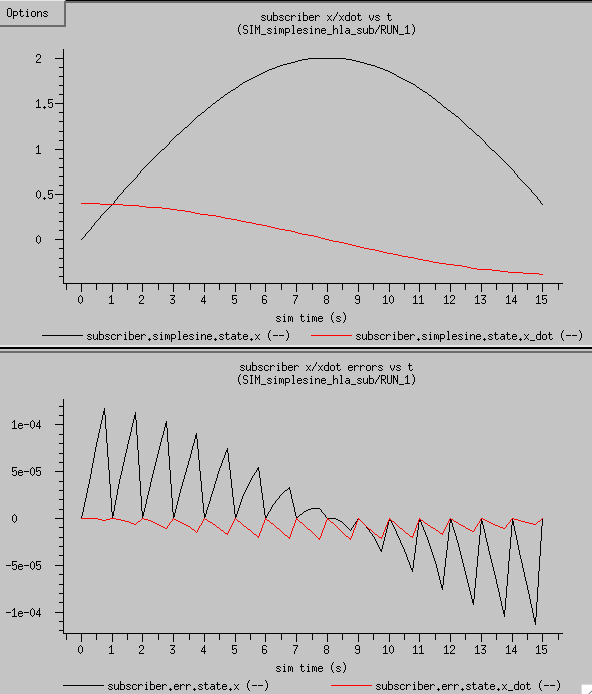
\includegraphics[width=4.5in]{TrickHLAUser-SIM-hla-pub-lagComp.png}
  \end{center}
\caption{Output from {\tt SIM\_simplesine\_hla\_pub\_lagComp}}
\label{fig:hla-pub-lagComp-output}
\end{figure}

\clearpage

% -------------------------------------------------------------------------
\section{Subscriber-resident Compensation}

This approach to lag compensation is handled by subscribers receiving
data from HLA.
Each subscriber is responsible for implementing their own logic for handling
the HLA-induced lag.
This section demonstrates how to do this.

% -----------------------------------
\subsection{{\tt SIM\_simplesine\_hla\_sub\_lagComp}}

This simulation illustrates what is required to implement
subscriber-side lag compensation in an existing (non-compensating)
simulation.
It is based on the {\tt SIM\_simplesine\_hla\_sub} simulation and differs
only in that the {\tt subscriber} sim object has a few new elements.

The sim object is shown in Listing~\ref{list:sub-lag-sim-object}.
The main differences between this simulation's \sdefine and that of the
subscriber discussed in Chapter~\ref{sec:hla-pubsub} are
\begin{itemize}
\item{
  the declaration of two \simplesine variables,
  one for uncompensated data and the other for compensated,
}
\item{
  the declaration of a {\em lag compensator} variable, and
}
\item{
  the initialization job for the lag compensator
}
\end{itemize}

\begin{lstlisting}[caption={{\tt subscriber} sim object for subscriber-side lag compensation},label={list:sub-lag-sim-object}]
sim_object
{
  sim_services/include: INTEGRATOR integ (simplesine/data/integ.d);
  simplesine: simplesine_T uncompensated_simplesine (simplesine/data/simplesine.d);
  simplesine: simplesine_T compensated_simplesine (simplesine/data/simplesine.d);
  simplesine: simplesine_T compensated_simplesine_error (simplesine/data/simplesine.d);
  simplesine: simplesine_LagCompensator lag_compensator;

  (initialization) simplesine:
    simplesine_calc(
      simplesine_T* P = &subscriber.uncompensated_simplesine,
      double t = sys.exec.out.time );
  (initialization) simplesine:
    simplesine_calc(
      simplesine_T* P = &subscriber.compensated_simplesine,
      double t = sys.exec.out.time );
  (initialization) simplesine:
    subscriber.lag_compensator.initialize(
      simplesine_T* uncompensatedP = &subscriber.uncompensated_simplesine,
      simplesine_T* compensatedP = &subscriber.compensated_simplesine );

  (derivative) simplesine:
    simplesine_deriv( simplesine_T* p = &subscriber.compensated_simplesine );
  (integration) simplesine:
    simplesine_integ(
      INTEGRATOR* I = &subscriber.integ,
      simplesine_T* p = &subscriber.compensated_simplesine );

  (PROPAGATE_TIMESTEP, scheduled) simplesine:
    simplesine_calcError(
      double t = sys.exec.out.time,
      simplesine_T* s = &subscriber.compensated_simplesine,
      simplesine_state_T* err = &subscriber.compensated_simplesine_error.state );
} subscriber ;
\end{lstlisting}

% -----------------------------------
\subsection{Input file}

The input file for the lag compensating subscriber is virtually identical
to the non-compensating subscriber with the following
exceptions.
\begin{itemize}
\item{
  The lag compensator defined in the \sdefine file is explicitly
  associated with the object being subscribed to and in particular is
  specified as a subscriber-resident (receiving) compensator by adding
  the following two lines to the input file:
  \begin{verbatim}
THLA.manager.objects[0].lag_comp      = &subscriber.lag_compensator;
THLA.manager.objects[0].lag_comp_type = THLA_LAG_COMP_RECEIVE_SIDE;
  \end{verbatim}
}
\item{
  Since the \sdefine for the compensating subscriber now includes
  uncompensated and the other compensated \simplesine variables,
  the lines in the input file which specify the Trick variable names
  to publish are changed accordingly from
  {\tt subscriber.simple\-sine} to
  {\tt sub\-scrib\-er.un\-compensated\_simplesine}.
}
\end{itemize}

Notice that the simulation subscribes to data from the publisher which are
saved in the {\em uncompensated} \simplesine variable, since the publisher
in this case does no lag compensation.
The \TrickHLA\ infrastructure takes care of executing the lag compensator,
which calculates the compensated \simplesine state by invoking
the {\tt simplesine\_LagCompensator} defined in the \sdefine file.

% -----------------------------------
\subsection{Output}

In this section,
we show the results of running a publisher,
{\tt SIM\_simplesine\_hla\_pub}
along with the lag-compensating
subscriber,
{\tt SIM\_simplesine\_hla\_sub\_lagComp}.

Again,
unlike Figure~\ref{fig:hla-sub-output} on page~\pageref{fig:hla-sub-output},
where the subscriber is out of phase with the true state,
in this case the subscriber's compensated sine wave is
in phase with the publisher
as shown in Figure~\ref{fig:hla-sub-lagComp-output}.

\begin{figure}[b]
  \begin{center}
    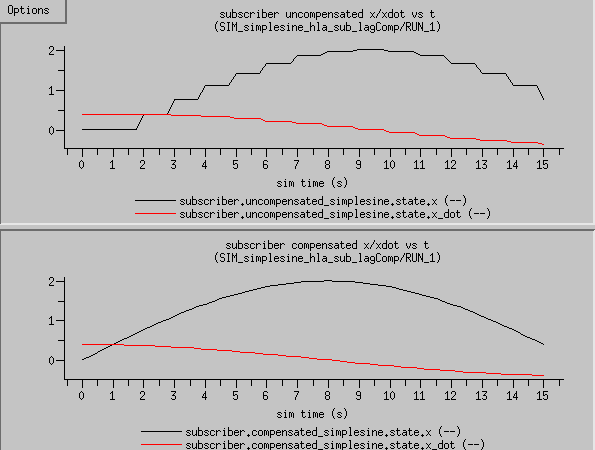
\includegraphics[width=4.5in]{TrickHLAUser-SIM-hla-sub-lagComp.png}
  \end{center}
\caption{Output from {\tt SIM\_simplesine\_hla\_sub\_lagComp}}
\label{fig:hla-sub-lagComp-output}
\end{figure}

\clearpage

\chapter{Sending and Receiving Interactions}
\label{sec:hla-inter}

This section illustrates how to use \TrickHLA\ to
send and receive HLA interactions.
The example simulations are similar to the publisher and
subscriber simulations discussed earlier, but in this case,
the subscriber's sine parameters have been initialized with
a zero-value amplitude.
Thus, the subscriber's state is initially constant,
$x(t)=0$, $\dot{x}(t)=0$.
However, at a certain point in the simulation,
the publisher sends its sine parameters
(in particular, a non-zero amplitude)
to the subscriber in an interaction.
Once the subscriber receives these values and updates the appropriate
Trick variables, $x(t)$ and $\dot{x}(t)$ assume their expected sine wave
shapes.\footnote{
  No state data are exchanged in this interaction, only the
  \simplesine parameters, $A$, $\phi$ and $\omega$.
  The calculation of the state on the subscriber side is only used as a
  way to graphically illustrate the arrival of the interaction from the
  publisher.
}

% -----------------------------------------------------------------------
\section{What is an interaction handler?}
% -------------------------------
\subsection{The class {\tt TrickHLAInteractionHandler}}

\TrickHLA\ defines a C++ class which may be subclassed by
simulation developers in order to send or receive interactions.
The class header is shown below.
It defines {\em send} and {\em receive} methods which may be called
by simulation developers,
avoiding the need to directly use the {\tt TrickHLAInteraction} class,
which is fairly complex.

There are actually two send methods.
The one with no arguments, sends the interaction to the receiver,
where it is delivered in the order interactions arrive off the network.
The send method with a single timetag argument sends the interaction
to receivers where it is delivered in time stamp order.
The timetag argument must be a simulation timetag plus some lookahead
interval.
These send methods are sufficient unto themselves and do not need to
be overridden in a subclass. Indeed they are not virtual methods.

The receive method is virtual.
The \TrickHLA\ infrastructure will automatically invoke a subclass's
corresponding version of the method when interactions arrive from remote
senders.

The protected {\tt interaction} field may be ignored.
The \TrickHLA\ infrastructure automatically takes care of creating
interactions according to the declarations encountered in the input file.

\begin{lstlisting}[caption={The {\tt TrickHLAInteractionHandler} class},label={list:trickhla-interaction-handler}]
class TrickHLAInteraction;
#include "TrickHLA/include/TrickHLAInteraction.hh"

class TrickHLAInteractionHandler
{
   friend class InputProcessor;
   friend void init_attrTrickHLAInteractionHandler();

  public:
   TrickHLAInteractionHandler();
   virtual ~TrickHLAInteractionHandler();

   virtual void initialize_callback( TrickHLAInteraction * inter );

   bool send_interaction(); // Receive Order
   bool send_interaction( double send_time ); // Timestamp Order

   TrickHLADoubleInterval get_fed_lookahead();
   TrickHLADoubleTime     get_granted_fed_time();
   
   virtual void receive_interaction();

  protected:
   TrickHLAInteraction * interaction;
};
\end{lstlisting}

% -------------------------------
\subsection{Interaction handling in \simplesine}

The class header for the \simplesine interaction handler is shown below.


\begin{lstlisting}[caption={{\tt simplesine\_InteractionHandler} header file},label={list:simplesine-interaction-handler-header}]
#include "TrickHLA/include/TrickHLAInteractionHandler.hh"

class simplesine_InteractionHandler : public TrickHLAInteractionHandler
{
  friend class InputProcessor;
  friend void init_attrsimplesine_InteractionHandler();

  public:
    simplesine_InteractionHandler();
    virtual ~simplesine_InteractionHandler();

    void send_sine_interaction( double send_time );
    virtual void receive_interaction();

  protected:
    double lookahead_time;
};
\end{lstlisting}

And the methods are shown below.
The {\tt send\_sine\_interaction()} method is just a wrapper around the
parent class's {\tt send\_interaction()} method.

And the {\tt receive\_interaction()} method, just invokes the Trick
output function, {\tt send\_hs()} to indicate that an interaction arrived;
by the time the receive method is invoked,
the data from the incoming interaction have already been stored in the
Trick variable that is associated with the interaction in the input
file. (See below.)
So there is nothing much to do in the implementation of the receive method.

\begin{lstlisting}[caption={{\tt simplesine\_InteractionHandler} methods},label={list:simplesine-interaction-handler-methods}]
/********************************* TRICK HEADER *******************************
PURPOSE: (Send/receive HLA interactions.)
*******************************************************************************/

#include <stdlib.h>
#include <string>
#include "../include/simplesine_InteractionHandler.hh"

using namespace std;

/* ----------------------------------------------------------------------------
PURPOSE: (Default constructor)
------------------------------------------------------------------------------*/
simplesine_InteractionHandler::simplesine_InteractionHandler() // RETURN: -- None.
: lookahead_time(0.0)
{ }


/* ----------------------------------------------------------------------------
PURPOSE: (Destructor.)
------------------------------------------------------------------------------*/
simplesine_InteractionHandler::~simplesine_InteractionHandler() // RETURN: -- None.
{ }


/* ----------------------------------------------------------------------------
PURPOSE: (Send this handler's HLA interaction. A pointer to the interaction
  is stored in this class -- defined in the protected <interaction> field
  in the parent class. The TrickHLA infrastructure takes care of setting
  that pointer when it sees interactions declared in the Trick input file.)
------------------------------------------------------------------------------*/
void simplesine_InteractionHandler::send_sine_interaction( // RETURN: -- None.
   double send_time )        // IN: s HLA time to send the interaction.
{
   const char* FOM_name = (const char*)this->interaction->get_FOM_name();
   bool interaction_was_sent = false;
   double timetag = send_time + lookahead_time;

   bool was_sent = this->TrickHLAInteractionHandler::send_interaction( timetag );

   if( was_sent ) {
      const char* msg = string("sent interaction: ").append(FOM_name).c_str();
      send_hs( stdout, (char*)msg );
   } else {
      const char* msg = string("error sending interaction: ").append(FOM_name).c_str();
      send_hs( stderr, (char*)msg );
   }
}


/* ----------------------------------------------------------------------------
PURPOSE: (Handle an incoming interaction.)
------------------------------------------------------------------------------*/
void simplesine_InteractionHandler::receive_interaction() // RETURN: -- None.
{
   const char* FOM_name = (const char*)this->interaction->get_FOM_name();
   const char* msg = string("Received interaction: ").append(FOM_name).c_str();

   send_hs( stdout, (char*)msg );
}
\end{lstlisting}

% -----------------------------------------------------------------------
\section{\tt SIM\_simplesine\_hla\_sendInt}

This simulation is based on the publisher simulation,
{\tt SIM\_simplesine\_hla\_pub} even though it does no real publishing.
Instead, it just sends an interaction once during the simulation.
The interaction handler {\em send} method is invoked at a specified
time during the simulation, using the Trick {\tt CALL} directive.\footnote{
  More sophisticated simulations might call the method
  directly from simulation-specific code.
  We do not do that here.
}
To do this, you must do two things to the \sdefine file.

\begin{itemize}
\item{
  Define an instance of the interaction handler, and
}
\item{
  Specify a 0-frequency job for the {\em send} method.\footnote{
    0-frequency jobs are a common way to force Trick to generate
    code for the job even though it is not actually part of the
    periodically scheduled jobs.
    In this case,
    the send method is not invoked from a regularly scheduled job,
    but from a single invocation of it as specified in the input file.
    If we did not specify a 0-frequency job like this, Trick would
    not compile the code for the job, and we would get a runtime error.
  }
}
\end{itemize}

Thus, the {\tt publisher} sim object for this simulation has two
lines that do not appear in the plain publisher:

\begin{lstlisting}[numbers=none,caption={Sending interaction handler \sdefine changes},label={list:sending-interaction-handler-sdefine-changed}]
  sim_object {
    ...
    simplesine: simplesine_InteractionHandler interaction_handler;
    ...
    (0.0, scheduled) simplesine:
      publisher.interaction_handler.send_sine_interaction(
        In double time = sys.exec.out.time );
    ...
} publisher;
\end{lstlisting}

% -----------------------------------------------------------------------
\section{Sender input}

The sender's input file is based on the plain publisher's input file.
They differ in the following ways.
\begin{itemize}
\item{
  The federate name is {\em sender} instead of {\em publisher},
  and it waits for the {\em receiver} federate instead of {\em subscriber},
}
\item{
  since this simulation does not actually publish anything,
  there are no objects and attributes defined,
}
\item{
  the interaction handler lookahead time is specified,
}
\item{
  the interaction and parameters to be sent are specified, and
}
\item{
  there is a {\tt CALL} directive invoking the interaction handler
  method, {\tt send\_sine\_interaction()}.
}
\end{itemize}

The complete input file is listed in
Appendix~\ref{sec:send-receive-inputs}
on page~\pageref{sec:complete-sender-input}.

% -----------------------------------------------------------------------
\section{\tt SIM\_simplesine\_hla\_receiveInt}

This simulation is based on the plain subscriber simulation,
{\tt SIM\_simplesine\_hla\_sub} even though it does no real subscribing.
Instead, it just waits for an interaction to arrive.
The \TrickHLA\ infrastructure automatically handles incoming interactions
and assigns the associated parameter values to Trick variables
as specified in the input file. (See next section.)
There are no explicit jobs to schedule in the \sdefine file,
and there are no jobs to {\tt CALL} from the input file, either.

To do this, all you need to do is declare an interaction handler
in the {\tt subscriber} sim object.\footnote{
  Unlike the case of sending interactions,
  receiving interactions requires no jobs be executed by Trick.
  Consequently, in this case (unlike the interaction sender),
  there is no need to declare a zero-frequency job in the \sdefine file.
}

The \sdefine for the receiver is virtually identical with that of the
plain subscriber with the following exceptions.

\begin{itemize}
\item{
A interaction handler variable is defined:
\begin{verbatim}
 simplesine: simplesine_InteractionHandler interaction_handler;
\end{verbatim}
}
\item{
The numerical integration of the the plain subscriber's state
has been replaced with the analytical propagation, since this
method is sensitive to changes in the parameters, whereas the
numerical integration of the state does not sense changes in the value
of the amplitude parameter.
}
\end{itemize}

this \sdefine file for this simulation is the same as the plain subscriber's.
% -----------------------------------------------------------------------
\section{Receiver input}

The receiver's input file is based on the plain subscriber's input file.
They differ in the following ways.
\begin{itemize}
\item{
  The federate name is {\em receiver} instead of {\em subscriber},
  and it waits for the {\em sender} federate instead of {\em publisher},
}
\item{
  since this simulation does not actually subscribe to anything,
  there are no objects and attributes defined, and
}
\item{
  the interaction and parameters to be sent are specified.
}
\end{itemize}

The complete input file is listed in
Appendix~\ref{sec:send-receive-inputs}
on page~\pageref{sec:complete-receiver-input}.

In addition,
for this simulation, the initial \simplesine amplitude parameter
is initialized to zero
(in the {\tt subscriber.d} initialization file included from the input file).
Until an incoming interaction resets the parameters,
the receiver's $x(t)$ and $\dot{x}(t)$ will be constant zero-valued functions
until a non-zero amplitude parameter arrives in an interaction from
from the sender.

% -----------------------------------------------------------------------
\section{Output}

Output from the sender shown below reveals that it does indeed send an interaction to the federation at $t=4$.

\begin{lstlisting}[numbers=none,caption={{\em sender} output showing interaction at $t=4$}]
...
| |wormhole|1|0.00|2007/08/03,22:27:05| TrickHLAManager::initialization_complete()
        Simulation has started and is now running...
| |wormhole|1|0.00|2007/08/03,22:27:05| TrickHLAManager::receive_cyclic_data()
| |wormhole|1|0.00|2007/08/03,22:27:05| TrickHLAManager::send_cyclic_and_requested_data()
| |wormhole|-1|0.25|2007/08/03,22:27:05| TrickHLAFedAmb::timeAdvanceGrant()
Federate "sender" Time granted to: 1
| |wormhole|1|1.00|2007/08/03,22:27:06| TrickHLAManager::receive_cyclic_data()
| |wormhole|1|1.00|2007/08/03,22:27:06| TrickHLAManager::send_cyclic_and_requested_data()
| |wormhole|-1|1.25|2007/08/03,22:27:06| TrickHLAFedAmb::timeAdvanceGrant()
Federate "sender" Time granted to: 2
| |wormhole|1|2.00|2007/08/03,22:27:07| TrickHLAManager::receive_cyclic_data()
| |wormhole|1|2.00|2007/08/03,22:27:07| TrickHLAManager::send_cyclic_and_requested_data()
| |wormhole|-1|2.25|2007/08/03,22:27:07| TrickHLAFedAmb::timeAdvanceGrant()
Federate "sender" Time granted to: 3
| |wormhole|1|3.00|2007/08/03,22:27:08| TrickHLAManager::receive_cyclic_data()
| |wormhole|1|3.00|2007/08/03,22:27:08| TrickHLAManager::send_cyclic_and_requested_data()
| |wormhole|-1|3.25|2007/08/03,22:27:08| TrickHLAFedAmb::timeAdvanceGrant()
Federate "sender" Time granted to: 4
| |wormhole|1|4.00|2007/08/03,22:27:09| TrickHLAInteraction::send() Timestamp Order:
      Interaction 'SimplesineParameters' sent for time 4.999 seconds.
| |wormhole|1|4.00|2007/08/03,22:27:09| sent interaction: SimplesineParameters
| |wormhole|1|4.00|2007/08/03,22:27:09| TrickHLAManager::receive_cyclic_data()
| |wormhole|1|4.00|2007/08/03,22:27:09| TrickHLAManager::send_cyclic_and_requested_data()
| |wormhole|-1|4.25|2007/08/03,22:27:09| TrickHLAFedAmb::timeAdvanceGrant()
Federate "sender" Time granted to: 5
...
\end{lstlisting}

Similarly, output from the receiver shown below reveals that
the interaction did indeed arrive.

\begin{lstlisting}[numbers=none,caption={{\em receiver} output showing interaction at $t=4$}]
...
| |wormhole|1|0.00|2007/08/03,22:27:05| TrickHLAManager::initialization_complete()
        Simulation has started and is now running...
| |wormhole|1|0.00|2007/08/03,22:27:05| TrickHLAManager::receive_cyclic_data()
| |wormhole|1|0.00|2007/08/03,22:27:05| TrickHLAManager::send_cyclic_and_requested_data()
| |wormhole|-1|0.25|2007/08/03,22:27:05| TrickHLAFedAmb::timeAdvanceGrant()
Federate "receiver" Time granted to: 1
| |wormhole|1|1.00|2007/08/03,22:27:06| TrickHLAManager::receive_cyclic_data()
| |wormhole|1|1.00|2007/08/03,22:27:06| TrickHLAManager::send_cyclic_and_requested_data()
| |wormhole|-1|1.25|2007/08/03,22:27:06| TrickHLAFedAmb::timeAdvanceGrant()
Federate "receiver" Time granted to: 2
| |wormhole|1|2.00|2007/08/03,22:27:07| TrickHLAManager::receive_cyclic_data()
| |wormhole|1|2.00|2007/08/03,22:27:07| TrickHLAManager::send_cyclic_and_requested_data()
| |wormhole|-1|2.25|2007/08/03,22:27:07| TrickHLAFedAmb::timeAdvanceGrant()
Federate "receiver" Time granted to: 3
| |wormhole|1|3.00|2007/08/03,22:27:08| TrickHLAManager::receive_cyclic_data()
| |wormhole|1|3.00|2007/08/03,22:27:08| TrickHLAManager::send_cyclic_and_requested_data()
| |wormhole|-1|3.25|2007/08/03,22:27:08| TrickHLAFedAmb::timeAdvanceGrant()
Federate "receiver" Time granted to: 4
| |wormhole|1|4.00|2007/08/03,22:27:09| TrickHLAManager::receive_cyclic_data()
| |wormhole|1|4.00|2007/08/03,22:27:09| TrickHLAManager::send_cyclic_and_requested_data()
| |wormhole|-1|4.25|2007/08/03,22:27:09| TrickHLAManager::receive_TSO_interaction() ID:77, HLA time:4.999
| |wormhole|-1|4.25|2007/08/03,22:27:09| TrickHLAFedAmb::timeAdvanceGrant()
Federate "receiver" Time granted to: 5
...
\end{lstlisting}

Note that the interaction has a timestamp of 4.999, which is
$t_{sim} + t_{lookahead}$.
(The lookahead is set to 1.000sec in the sender's input file.)

Finally, the plot below shows the analytically propagated subscriber state.
In particular, it reveals that upon arrival of the parameter values
at $t=4.999$, the functions $x(t)$ and $\dot{x}(t)$ pick up their expected
sine wave forms, confirming the arrival of the interaction.

\begin{figure}[h]
  \begin{center}
    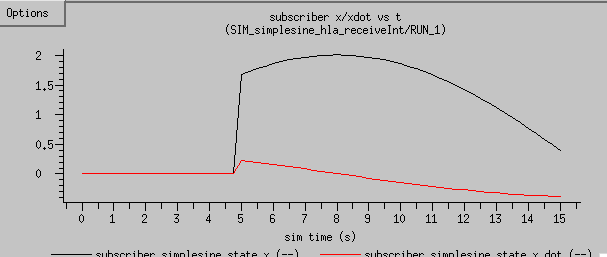
\includegraphics[width=4.5in]{TrickHLAUser-receiveInt.png}
  \end{center}
\caption{$x(t)$ and $\dot{x}(t)$ from {\tt SIM\_simplesine\_hla\_receiveInt}}
\label{fig:hla-receiveInt}
\end{figure}

\chapter{Ownership Transfer}
\label{sec:hla-own}

There are two \TrickHLA\ mechanisms for initiating ownership transfer:
the current owner may {\em divest} itself of ownership contingent on the
existence of some other federate that is willing to assume it,
or a non-owner may {\em acquire} ownership from the current owner
contingent on that federate being willing.
The \TrickHLA\ terminology for these two approaches to ownership  transfer
is {\em push} and {\em pull}, respectively.
This chapter illustrates how to write simulations that push and/or pull
ownership.

The simulations we present are
\begin{itemize}
\item{
  A publisher that initially owns the \simplesine state
  and {\em pushes} ownership away at a specified time in the run
  then at some subsequent time {\em pulls} ownership back, and
}
\item{
  Another publisher that does not initially own the \simplesine state
  but will assume ownership when the other federate divests it and will
  surrender it when the original federate tries to pull ownership back.
}
\end{itemize}

\TrickHLA\ automatically ensures that publishers
(federates who explicitly indicate their {\em ability}
to update the associated data)
are eligible to assume ownership when the current owner divests
itself of ownership by invoking the \TrickHLA\ {\em push} method.
The non-owning publisher does not need to take any explicit action
for this to happen.\footnote{
  Thus, in the HLA nomenclature, the distinction between a
  publisher that {\em owns} the object/attributes and a
  publisher that {\em does not own} them is important.
  For former may generate updates for them, and the latter may not.
  Thus, ownership tranfer leads to a change in which publisher
  is actually generating data updates.
}
Similarly, when a non-owning publisher invokes the
\TrickHLA\ {\em pull} method, transfer of ownership from the current owner
to the requesting federate is automatically handled.
The current owner needs not explicitly handle the transfer request.\footnote{
  Indeed, \TrickHLA\ does not currently provide any mechanism
  for the current owner to decline a pull request.
}

% ---------------------------------------------------------------------
\section{What is an ownership handler?}

\TrickHLA\ includes a utility class that may be used directly
(i.e., no subclassing necessary)
to push and pull ownership.
The class header is shown below.

\begin{lstlisting}[caption={{\tt TrickHLAOwnershipHandler} class header}]
#include <string>

#include "TrickHLA/include/TrickHLAStandardsSupport.hh"
class TrickHLAObject;
class TrickHLAAttribute;
#include "TrickHLA/include/TrickHLAObject.hh"
#include "TrickHLA/include/TrickHLAAttribute.hh"
#include "TrickHLA/include/TrickHLATypesNoICG.hh"
#include "TrickHLA/include/TrickHLAOwnershipHandlerNoICG.hh"
#include "TrickHLA/include/TrickHLAOwnershipItem.hh"
#include "TrickHLA/include/TrickHLADoubleInterval.hh"
#include "TrickHLA/include/TrickHLADoubleTime.hh"

#include RTI1516_HEADER

using namespace std;
using namespace RTI1516_NAMESPACE;

class TrickHLAOwnershipHandler
{
  friend class InputProcessor;
  friend void init_attrTrickHLAOwnershipHandler();

  friend class TrickHLAObject;
  
  public:
   TrickHLAOwnershipHandler();
   virtual ~TrickHLAOwnershipHandler();

   void checkpoint_requests();
   void clear_checkpoint();
   void restore_requests();
   
   virtual void initialize_callback( TrickHLAObject * obj );

   string get_object_name();
   string get_object_FOM_name();

   int get_attribute_count();
   VectorOfStrings get_attribute_FOM_names() const;

   bool is_locally_owned( const char * attribute_FOM_name );
   bool is_remotely_owned( const char * attribute_FOM_name );

   bool is_published( const char * attribute_FOM_name );
   bool is_subscribed( const char * attribute_FOM_name );

   void pull_ownership();
   void pull_ownership( double time );
   void pull_ownership( const char * attribute_FOM_name );
   void pull_ownership( const char * attribute_FOM_name, double time );

   void push_ownership();
   void push_ownership( double time );
   void push_ownership( const char * attribute_FOM_name );
   void push_ownership( const char * attribute_FOM_name, double time );

   TrickHLADoubleInterval get_fed_lookahead();
   TrickHLADoubleTime     get_granted_fed_time();

  private:
   TrickHLAAttribute * get_attribute( const char * attribute_FOM_name );
   TrickHLAObject * object;    // ** Reference to the TrickHLA Object.
   AttributeOwnershipMap pull_requests; // ** Map of pull ownership user requests.
   AttributeOwnershipMap push_requests; // ** Map of push ownership user requests.
   int                     pull_items_cnt; // -- # of pull items
   TrickHLAOwnershipItem * pull_items;     // -- array of pulled attributes
   int                     push_items_cnt; // -- # of push items
   TrickHLAOwnershipItem * push_items;     // -- array of pushed attributes
};
\end{lstlisting}

The {\tt pull\_ownership()} and {\tt push\_ownership()} methods are of
particular interest.
The methods without arguments push or pull all the attributes of the
associated object immediately.
The methods with only a time argument push or pull all the attributes of the
specific object at the specified future time.
And the methods with an explicit attribute name argument allow pushing and
pulling of single attributes within an object without affecting the others.

% ---------------------------------------------------------------------
\section{\tt SIM\_simplesine\_hla\_own}

Our illustration of how to use the {\tt TrickHLAOwnershipHandler} class
involves two different instances of a single simulation.

The first instance is the {\em active} publisher that
initially owns the relevant object and attributes
and explicitly calls the {\tt push\_ownership()} and {\tt pull\_ownership()}
methods.
The second instance is a {\em passive} publisher that does not initially
own the object and attributes, nor does it explicitly request any ownership
transfers.
Instead, the passive instance of the simulation gains and surrenders
ownership as the result of the remote push/pull requests by the active
instance.

Both instances not only publish the \simplesine data, but they also
subscribe, allowing them to receive updates from the other instance
when the object and attributes are remotely owned.

The two instances share the same \sdefine file, which is derived from
the plain publisher.
The only differences between the \sdefine file for the
{\tt SIM\_simplesine\_hla\_own} simulation
and that of the plain publisher are

\begin{itemize}
\item{
  an ownership handler variable is defined by adding the following line,
  \begin{verbatim}
 TrickHLA: TrickHLAOwnershipHandler ownership_handler; \end{verbatim}
}
\item{
  and zero-frequency jobs are declared for
  {\tt push\_ownership()} and {\tt pull\_ownership()}
  as follows
  \begin{verbatim}
 (0.0, scheduled) TrickHLA: publisher.ownership_handler.push_ownership();
 (0.0, scheduled) TrickHLA: publisher.ownership_handler.pull_ownership(); \end{verbatim}
  so that the methods may be invoked from the input file using the
  {\tt CALL} directive.
}
\end{itemize}

% ---------------------------------------------------------------------
\section{Active input file}

The input file for the active ownership transfer simulation is
based on the input file for the plain publisher.
The differences are:

\begin{itemize}
\item{
  A new file, {\tt LogData/THLA\_objects.d} is included.
  This file contains inputs that ensure that the ownership flag
  {\tt THLA.manager.objects[0].attributes[0].locally\_owned} is logged.
  This allows us to plot the ownership transfer as it takes place.
}
\item{
  The federate name is {\em active} instead of {\em publisher}.
}
\item{
  The federate waits for a second federate named {\em passive}
  instead of {\em subscriber}.
}
\item{
  The ownership handler defined in the \sdefine file is associated
  with the object as follows.
  \begin{verbatim}
  THLA.manager.objects[0].ownership = &publisher.ownership_handler; \end{verbatim}
}
\item{
  The {\tt .subscribe} flag of the object's attributes are all set to
  true so that the simulation will receive updated values when the
  other federate owns the object.
}
\item{
  The simulation {\em pushes} ownership away at $t=5$ using the {\tt CALL}
  directive as follows.
  \begin{verbatim}
 read = 5.0;
 CALL publisher.publisher.ownership_handler.push_ownership(); \end{verbatim}
}
\item{
  And finally the simulation {\em pulls} ownership back at $t=10$
  as follows.
  \begin{verbatim}
 read = 10.0;
 CALL publisher.publisher.ownership_handler.pull_ownership(); \end{verbatim}
}
\end{itemize}

% ---------------------------------------------------------------------
\section{Passive input file}

The input file for the passive ownership transfer simulation is
virtually identical to the active input file with the following exceptions.

\begin{itemize}
\item{
  The federate name is {\em passive}.
}
\item{
  The attribute {\tt .locally\_owned} flags are initially false,
  since at simulation start the passive simulation does not own them.
}
\item{
  There are no {\tt CALL} directives.
}
\end{itemize}

That last point deserves emphasizing.
This simulation accepts ownership when the {\em active} federate pushes
ownership away from itself; no explicit action is required on the part
of the passive simulation in order to accept ownerhip.
Similarly,
this simulation willingly surrenders ownership when the {\em active}
federate pulls it back; again, this happens without any explicit action
on the part of the passive simulation.

% ---------------------------------------------------------------------
\section{Output}

Inspection of the (abbreviated) output shown below from the active simulation
reveals that it does indeed divest ownership and then reacquire it later.

\begin{lstlisting}[numbers=none,caption={Output stream from the active ownerhsip transfer simulation}]
...
| |wormhole|1|3.00|2007/08/05,21:56:18| TrickHLAManager::receive_cyclic_data()
| |wormhole|1|3.00|2007/08/05,21:56:18| TrickHLAManager::send_cyclic_data()
| |wormhole|-1|3.25|2007/08/05,21:56:18| TrickHLAFedAmb::timeAdvanceGrant()
Federate "active" Time granted to: 4
| |wormhole|1|4.00|2007/08/05,21:56:19| TrickHLAManager::receive_cyclic_data()
| |wormhole|1|4.00|2007/08/05,21:56:19| TrickHLAManager::send_cyclic_data()
| |wormhole|-1|4.25|2007/08/05,21:56:19| TrickHLAFedAmb::timeAdvanceGrant()
Federate "active" Time granted to: 5
| |wormhole|1|5.00|2007/08/05,21:56:20| TrickHLAManager::receive_cyclic_data()
| |wormhole|1|5.00|2007/08/05,21:56:20| TrickHLAManager::send_cyclic_data()
| |wormhole|1|5.00|2007/08/05,21:56:20| TrickHLAObject::push_ownership()
...
| |wormhole|1|6.00|2007/08/05,21:56:21| TrickHLAObject::release_ownership()
   DIVESTED Ownership of attribute 'SimplesineStateAndParameters'->'Time'
   of object 'simplesineStateAndParameters'.
| |wormhole|1|6.00|2007/08/05,21:56:21| TrickHLAObject::release_ownership()
   DIVESTED Ownership of attribute 'SimplesineStateAndParameters'->'Value'
   of object 'simplesineStateAndParameters'.
| |wormhole|1|6.00|2007/08/05,21:56:21| TrickHLAObject::release_ownership()
   DIVESTED Ownership of attribute 'SimplesineStateAndParameters'->'dvdt'
   of object 'simplesineStateAndParameters'.
| |wormhole|1|6.00|2007/08/05,21:56:21| TrickHLAObject::release_ownership()
   DIVESTED Ownership of attribute 'SimplesineStateAndParameters'->'Phase'
   of object 'simplesineStateAndParameters'.
| |wormhole|1|6.00|2007/08/05,21:56:21| TrickHLAObject::release_ownership()
   DIVESTED Ownership of attribute 'SimplesineStateAndParameters'->'Frequency'
   of object 'simplesineStateAndParameters'.
| |wormhole|1|6.00|2007/08/05,21:56:21| TrickHLAObject::release_ownership()
   DIVESTED Ownership of attribute 'SimplesineStateAndParameters'->'Amplitude'
   of object 'simplesineStateAndParameters'.
...
| |wormhole|1|9.00|2007/08/05,21:56:24| TrickHLAManager::receive_cyclic_data()
| |wormhole|1|9.00|2007/08/05,21:56:24| TrickHLAManager::send_cyclic_data()
| |wormhole|-1|9.25|2007/08/05,21:56:24| TrickHLAFedAmb::timeAdvanceGrant()
Federate "active" Time granted to: 10
| |wormhole|1|10.00|2007/08/05,21:56:25| TrickHLAManager::receive_cyclic_data()
| |wormhole|1|10.00|2007/08/05,21:56:25| TrickHLAManager::send_cyclic_data()
| |wormhole|1|10.00|2007/08/05,21:56:25| TrickHLAObject::pull_ownership()
...
   ACQUIRED ownership of attribute 'SimplesineStateAndParameters'->'Time'
   of object 'simplesineStateAndParameters'.
| |wormhole|-1|11.25|2007/08/05,21:56:26| TrickHLAFedAmb::attributeOwnershipAcquisitionNotification()
   ACQUIRED ownership of attribute 'SimplesineStateAndParameters'->'Value'
   of object 'simplesineStateAndParameters'.
| |wormhole|-1|11.25|2007/08/05,21:56:26| TrickHLAFedAmb::attributeOwnershipAcquisitionNotification()
   ACQUIRED ownership of attribute 'SimplesineStateAndParameters'->'dvdt'
   of object 'simplesineStateAndParameters'.
| |wormhole|-1|11.25|2007/08/05,21:56:26| TrickHLAFedAmb::attributeOwnershipAcquisitionNotification()
   ACQUIRED ownership of attribute 'SimplesineStateAndParameters'->'Phase'
   of object 'simplesineStateAndParameters'.
| |wormhole|-1|11.25|2007/08/05,21:56:26| TrickHLAFedAmb::attributeOwnershipAcquisitionNotification()
   ACQUIRED ownership of attribute 'SimplesineStateAndParameters'->'Frequency'
   of object 'simplesineStateAndParameters'.
| |wormhole|-1|11.25|2007/08/05,21:56:26| TrickHLAFedAmb::attributeOwnershipAcquisitionNotification()
   ACQUIRED ownership of attribute 'SimplesineStateAndParameters'->'Amplitude'
   of object 'simplesineStateAndParameters'.
...
\end{lstlisting}

On the other side,
inspection of the (abbreviated) output shown below from the passive simulation
reveals that it does indeed acquire ownership and then divest it later.

\begin{lstlisting}[numbers=none,caption={Output stream from the passive ownerhsip transfer simulation}]
...
| |wormhole|1|4.00|2007/08/05,21:56:19| TrickHLAManager::receive_cyclic_data()
| |wormhole|1|4.00|2007/08/05,21:56:19| TrickHLAManager::send_cyclic_data()
| |wormhole|-1|4.25|2007/08/05,21:56:19| TrickHLAFedAmb::timeAdvanceGrant()
Federate "passive" Time granted to: 5
| |wormhole|1|5.00|2007/08/05,21:56:20| TrickHLAManager::receive_cyclic_data()
| |wormhole|1|5.00|2007/08/05,21:56:20| TrickHLAManager::send_cyclic_data()
| |wormhole|-1|5.25|2007/08/05,21:56:20| TrickHLAFedAmb::timeAdvanceGrant()
Federate "passive" Time granted to: 6
| |wormhole|-1|5.25|2007/08/05,21:56:20| TrickHLAFedAmb::requestAttributeOwnershipAssumption()
  push request received, tag='simplesineStateAndParameters'
| |wormhole|-1|5.25|2007/08/05,21:56:20| TrickHLAFedAmb::requestAttributeOwnershipAssumption()
...
| |wormhole|-1|6.25|2007/08/05,21:56:21| TrickHLAFedAmb::attributeOwnershipAcquisitionNotification()
   ACQUIRED ownership of attribute 'SimplesineStateAndParameters'->'Time'
   of object 'simplesineStateAndParameters'.
| |wormhole|-1|6.25|2007/08/05,21:56:21| TrickHLAFedAmb::attributeOwnershipAcquisitionNotification()
   ACQUIRED ownership of attribute 'SimplesineStateAndParameters'->'Value'
   of object 'simplesineStateAndParameters'.
| |wormhole|-1|6.25|2007/08/05,21:56:21| TrickHLAFedAmb::attributeOwnershipAcquisitionNotification()
   ACQUIRED ownership of attribute 'SimplesineStateAndParameters'->'dvdt'
   of object 'simplesineStateAndParameters'.
| |wormhole|-1|6.25|2007/08/05,21:56:21| TrickHLAFedAmb::attributeOwnershipAcquisitionNotification()
   ACQUIRED ownership of attribute 'SimplesineStateAndParameters'->'Phase'
   of object 'simplesineStateAndParameters'.
| |wormhole|-1|6.25|2007/08/05,21:56:21| TrickHLAFedAmb::attributeOwnershipAcquisitionNotification()
   ACQUIRED ownership of attribute 'SimplesineStateAndParameters'->'Frequency'
   of object 'simplesineStateAndParameters'.
| |wormhole|-1|6.25|2007/08/05,21:56:21| TrickHLAFedAmb::attributeOwnershipAcquisitionNotification()
   ACQUIRED ownership of attribute 'SimplesineStateAndParameters'->'Amplitude'
   of object 'simplesineStateAndParameters'.
| |wormhole|-1|6.25|2007/08/05,21:56:21| TrickHLAFedAmb::timeAdvanceGrant()
Federate "passive" Time granted to: 7
...
| |wormhole|-1|10.25|2007/08/05,21:56:25| TrickHLAFedAmb::requestAttributeOwnershipRelease()
  pull request received, tag='simplesineStateAndParameters'
| |wormhole|-1|10.25|2007/08/05,21:56:25| TrickHLAFedAmb::requestAttributeOwnershipRelease()
...
   DIVESTED Ownership for attribute 'SimplesineStateAndParameters'->'Time'
   of object 'simplesineStateAndParameters'.
| |wormhole|1|11.00|2007/08/05,21:56:26| TrickHLAObject::grant_pull_request()
   DIVESTED Ownership for attribute 'SimplesineStateAndParameters'->'Value'
   of object 'simplesineStateAndParameters'.
| |wormhole|1|11.00|2007/08/05,21:56:26| TrickHLAObject::grant_pull_request()
   DIVESTED Ownership for attribute 'SimplesineStateAndParameters'->'dvdt'
   of object 'simplesineStateAndParameters'.
| |wormhole|1|11.00|2007/08/05,21:56:26| TrickHLAObject::grant_pull_request()
   DIVESTED Ownership for attribute 'SimplesineStateAndParameters'->'Phase'
   of object 'simplesineStateAndParameters'.
| |wormhole|1|11.00|2007/08/05,21:56:26| TrickHLAObject::grant_pull_request()
   DIVESTED Ownership for attribute 'SimplesineStateAndParameters'->'Frequency'
   of object 'simplesineStateAndParameters'.
| |wormhole|1|11.00|2007/08/05,21:56:26| TrickHLAObject::grant_pull_request()
   DIVESTED Ownership for attribute 'SimplesineStateAndParameters'->'Amplitude'
   of object 'simplesineStateAndParameters'.
...
\end{lstlisting}

This is also illustrated in the two following plots of the
{\tt .locally\_owned} flag for the first attribute of the object.

\clearpage

\begin{figure}[h]
  \begin{center}
    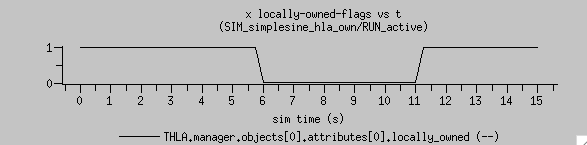
\includegraphics[width=5.5in]{TrickHLAUser-SIM-hla-own-active.png}
  \end{center}
\caption{Output from the active {\tt SIM\_simplesine\_hla\_own} simulation}
\label{fig:hla-own-active-output}
\end{figure}


\begin{figure}[h]
  \begin{center}
    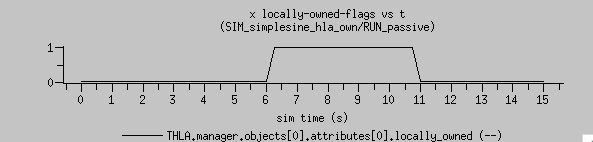
\includegraphics[width=5.5in]{TrickHLAUser-SIM-hla-own-passive.png}
  \end{center}
\caption{Output from the passive {\tt SIM\_simplesine\_hla\_own} simulation}
\label{fig:hla-own-passive-output}
\end{figure}

\clearpage

\chapter{Data Encoding and Packing}
\label{sec:hla-pack}

\TrickHLA\ provides a mechanism for simulation developers to
modify updated class attribute data before sending it out to other federates
or upon receiving new data from publishers.
This capability might be necessary, for example, if the agreed-upon units
for an attribute are different from those used internally by the simulation,
in which case a developer could write {\em pack} and {\em unpack} logic
to change units as data come into and leaves the simulation.
This chapter illustrates how to do that.

% ---------------------------------------------------------------------------
\section{What is a {\em packing} class?}

\TrickHLA\ provides two {\em hooks} that allow simulation developers
to modify\footnote{
  What {\em modify} means is application specific.
  It might be encoding/decoding.
  It might be packing/unpacking.
  Or it might be changing units back and forth from FOM-agreed units
  (e.g., degrees) and application-specific units (e.g., radians).
}
data as it is sent out via HLA
and as it arrives from HLA.
This is implemented in the {\tt pack()} and {\tt unpack()}
methods of the {\tt TrickHLAPacking} class.
The {\tt pack()} method is automatically invoked by
\TrickHLA\ before data are sent via HLA.
The {\tt unpack()} method is automatically invoked by
\TrickHLA\ after data are received from HLA.
These are virtual methods and must be overriden in a subclass
in order to add application-specific packing and unpacking to the simulation.

% ------------------------------------
\subsection{{\tt TrickHLAPacking}}

The header file for the {\tt TrickHLAPacking} class is shown below.

\begin{lstlisting}[caption={{\tt TrickHLAPacking} class header}]
class TrickHLAObject;
#include "TrickHLA/include/TrickHLAObject.hh"

class TrickHLAPacking
{
   friend class InputProcessor;
   friend void init_attrTrickHLAPacking();

  public:
   TrickHLAPacking() {};
   virtual ~TrickHLAPacking() {};

   TrickHLADebugHandler debug_handler; // -- Prints out multiple debug levels

   TrickHLAAttribute * get_attribute( const char * attr_FOM_name );

   virtual void initialize_callback( TrickHLAObject * obj );

   //-----------------------------------------------------------------
   // These are virtual functions and must be defined by a full class.
   //-----------------------------------------------------------------

   virtual void pack();

   virtual void unpack();

  protected:
   TrickHLAObject * object;   // ** Reference to the TrickHLA Object.
};
\end{lstlisting}

% ------------------------------------
\subsection{{\tt simplesine\_Packing}}

In order to illustrate the use of the {\tt TrickHLAPacking} class,
the \simplesine model has a packing class.
The class header is shown below.

\begin{lstlisting}[caption={{\tt simplesine\_Packing} class header}]
#include "TrickHLA/include/TrickHLAPacking.hh"
#include "simplesine/include/simplesine.h"

class simplesine_Packing : public TrickHLAPacking
{
  friend class InputProcessor;
  friend void init_attrsimplesine_Packing();

  public:
    simplesine_Packing();
    virtual ~simplesine_Packing();

    virtual void init(
      simplesine_T* originalP,
      simplesine_T* packedP,
      simplesine_T* unpackedP );

    virtual void pack();
    virtual void unpack();

  private:
    bool is_initialized;
    simplesine_T* originalP;
    simplesine_T* packedP;
    simplesine_T* unpackedP;
};
\end{lstlisting}

This class is designed to work as follows.
the {\tt init()} method {\em must} be called in order to initialize the class
(i.e., invoked as a Trick initialization job).
The initialization method specifies three \simplesine objects:
\begin{itemize}
\item{{\tt originalP} --
  The \simplesine data used as input to the {\tt pack()} and {\tt unpack()}
  methods.
}
\item{{\tt packedP} --
  The \simplesine data used as output from the {\tt pack()} method.
}
\item{{\tt unpackedP} --
  The \simplesine data used as output from the {\tt unpack()} method.
}
\end{itemize}

The implementation of the methods is shown below.
In this case, both methods just copy the data without doing any
modification at all, which of course has no value other than
illustrating (in the following simulations) how to use the
{\tt TrickHLAPacking} class.

\begin{lstlisting}[caption={{\tt simplesine\_Packing} class methods}]
/********************************* TRICK HEADER *******************************
PURPOSE: (implementation of packing/unpacking methods)
LIBRARY DEPENDENCY: ((simplesine_copy.o))
*******************************************************************************/
// System include files.
#include <math.h>
#include <stdlib.h>
#include <iostream>
#include <string>

// Trick include files.
#include "sim_services/include/exec_proto.h"

// TrickHLA model include files.
#include "TrickHLA/include/TrickHLAAttribute.hh"

// Model include files.
#include "../include/simplesine_Packing.hh"
#include "../include/simplesine_proto.h"

using namespace std;

/*----------------------------------------------------------------------------
PURPOSE: (default constructor for the simplesine packing/unpacking class.)
-----------------------------------------------------------------------------*/
simplesine_Packing::simplesine_Packing() // RETURN: -- None.
  : is_initialized(false),
    originalP(NULL),
    packedP(NULL),
    unpackedP(NULL)
{ }

/*----------------------------------------------------------------------------
PURPOSE: (destructor for the simplesine packing/unpacking class.)
-----------------------------------------------------------------------------*/
simplesine_Packing::~simplesine_Packing() // RETURN: -- None.
{ }

/*----------------------------------------------------------------------------
PURPOSE: (initialization method)
-----------------------------------------------------------------------------*/
void simplesine_Packing::init( // RETURN: -- None.
  simplesine_T* originalP,     // INOUT:  -- where the data is coming from
  simplesine_T* packedP,       // INOUT:  -- where to pack it into
  simplesine_T* unpackedP)     // INOUT:  -- where to unpack it into
{
  this->originalP = originalP;
  this->packedP = packedP;
  this->unpackedP = unpackedP;
  this->is_initialized = true;
}

/*----------------------------------------------------------------------------
PURPOSE: (data packing method.  This is called before data is sent to the RTI.)
-----------------------------------------------------------------------------*/
void simplesine_Packing::pack()  // RETURN: -- None.
{
  if( ! this->is_initialized ) {
    exec_terminate(
      "simplesine_Packing.cpp",
      "simplesine_Packing::pack() called on non-initialized object" );
  }

  send_hs( stdout, "pack(): packing data from %p into %p", originalP, packedP );
  simplesine_copy( originalP, packedP );
}

/*----------------------------------------------------------------------------
PURPOSE: (data unpacking method.  This is called after data is received
  from the RTI.)
-----------------------------------------------------------------------------*/
void simplesine_Packing::unpack() // RETURN: -- None.
{
  if( ! this->is_initialized ) {
    exec_terminate(
      "simplesine_Packing.cpp",
      "simplesine_Packing::unpack() called on non-initialized object" );
  }

  send_hs( stdout, "unpack(): unpacking data from %p into %p", originalP, unpackedP );
  simplesine_copy( originalP, unpackedP );
}
\end{lstlisting}

% ---------------------------------------------------------------------------
\section{\tt SIM\_simplesine\_hla\_pack}

This {\tt SIM\_simplesine\_hla\_pack} simulation illustrates how to
{\em pack} data from a publishing simulation.
The simulation is based on the plain publisher,
{\tt SIM\_simplesine\_hla\_pub}, from
Chapter~\ref{sec:hla-pubsub}.

% -----------------------
\subsection{\sdefine file}
This differences between the \sdefine for this simulation and that
of the plain publisher are as follows.

\begin{itemize}
\item{
  A new \simplesine variable, {\tt simplesine\_packed},
  is defined in the {\tt publisher} sim object.
}
\item{
  The definition of an instance, {\tt packer},
  of the {\tt simplesine\_Packing} class.
}
\item{
  The invocation of {\tt simplesine\_Packing::init()} as a Trick
  initialization job,
  specifying {\tt publisher.simplesine} as the input to the {\tt pack()}
  method and {\tt publisher.simple\-sine\_\-packed} as the output.
}
\end{itemize}

% -----------------------
\subsection{Input file}

The only difference between the input file for this simulation and
that of the plain publisher is the following new line

\begin{verbatim}
THLA.manager.objects[0].packing = &publisher.packer; \end{verbatim}

which associates {\tt publisher.packer} as the packing class for
the object being published.

% ---------------------------------------------------------------------------
\section{\tt SIM\_simplesine\_hla\_unpack}

This {\tt SIM\_simplesine\_hla\_unpack} simulation illustrates how to
{\em unpack} data from a subscribing simulation.
The simulation is based on the plain subscriber,
{\tt SIM\_simplesine\_hla\_sub}, from
Chapter~\ref{sec:hla-pubsub}.

% -----------------------
\subsection{\sdefine file}
This differences between the \sdefine for this simulation and that
of the plain subscriber are as follows.

\begin{itemize}
\item{
  A new \simplesine variable, {\tt simplesine\_unpacked},
  is defined in the {\tt subscriber} sim object.
}
\item{
  The definition of an instance, {\tt unpacker},
  of the {\tt simplesine\_Packing} class.
}
\item{
  The invocation of {\tt simplesine\_Packing::init()} as a Trick
  initialization job,
  specifying {\tt subscriber.simplesine} as the input to the {\tt unpack()}
  method and {\tt subscriber.simple\-sine\_\-un\-packed} as the output.
}
\end{itemize}

% -----------------------
\subsection{Input file}

The only difference between the input file for this simulation and
that of the plain subscriber is the following new line

\begin{verbatim}
THLA.manager.objects[0].packing = &subscriber.unpacker; \end{verbatim}

which associates {\tt subscriber.unpacker} as the packing class for
the object to which the simulation subscribes.

% ---------------------------------------------------------------------------
\section{Output}

The output of running the pack and unpack simulations
shows issued by the \simplesine {\tt pack()} and
{\tt unpack()} methods.

\begin{lstlisting}[numbers=none,caption={Output from the packer simulation}]
...
| |wormhole|1|0.00|2007/08/05,23:39:14| TrickHLAManager::initialization_complete()
        Simulation has started and is now running...
| |wormhole|1|0.00|2007/08/05,23:39:14| TrickHLAManager::receive_cyclic_data()
| |wormhole|1|0.00|2007/08/05,23:39:14| TrickHLAManager::send_cyclic_and_requested_data()
| |wormhole|1|0.00|2007/08/05,23:39:14| pack(): packing data from 0x99aaee4 into 0x99aaf1c
| |wormhole|-1|0.25|2007/08/05,23:39:14| TrickHLAFedAmb::timeAdvanceGrant()
Federate "publisher" Time granted to: 1
| |wormhole|1|1.00|2007/08/05,23:39:15| TrickHLAManager::receive_cyclic_data()
| |wormhole|1|1.00|2007/08/05,23:39:15| TrickHLAManager::send_cyclic_and_requested_data()
| |wormhole|1|1.00|2007/08/05,23:39:15| pack(): packing data from 0x99aaee4 into 0x99aaf1c
| |wormhole|-1|1.25|2007/08/05,23:39:15| TrickHLAFedAmb::timeAdvanceGrant()
Federate "publisher" Time granted to: 2
| |wormhole|1|2.00|2007/08/05,23:39:16| TrickHLAManager::receive_cyclic_data()
| |wormhole|1|2.00|2007/08/05,23:39:16| TrickHLAManager::send_cyclic_and_requested_data()
| |wormhole|1|2.00|2007/08/05,23:39:16| pack(): packing data from 0x99aaee4 into 0x99aaf1c
| |wormhole|-1|2.25|2007/08/05,23:39:16| TrickHLAFedAmb::timeAdvanceGrant()
Federate "publisher" Time granted to: 3
| |wormhole|1|3.00|2007/08/05,23:39:17| TrickHLAManager::receive_cyclic_data()
| |wormhole|1|3.00|2007/08/05,23:39:17| TrickHLAManager::send_cyclic_and_requested_data()
| |wormhole|1|3.00|2007/08/05,23:39:17| pack(): packing data from 0x99aaee4 into 0x99aaf1c
| |wormhole|-1|3.25|2007/08/05,23:39:17| TrickHLAFedAmb::timeAdvanceGrant()
Federate "publisher" Time granted to: 4
...
\end{lstlisting}

\begin{lstlisting}[numbers=none,caption={Output from the unpacker simulation}]
...
| |wormhole|1|0.00|2007/08/05,23:39:14| TrickHLAManager::initialization_complete()
        Simulation has started and is now running...
| |wormhole|1|0.00|2007/08/05,23:39:14| TrickHLAManager::receive_cyclic_data()
| |wormhole|1|0.00|2007/08/05,23:39:14| TrickHLAManager::send_cyclic_and_requested_data()
| |wormhole|1|0.00|2007/08/05,23:39:14| pack(): packing data from 0x99aaee4 into 0x99aaf1c
| |wormhole|-1|0.25|2007/08/05,23:39:14| TrickHLAFedAmb::timeAdvanceGrant()
Federate "publisher" Time granted to: 1
| |wormhole|1|1.00|2007/08/05,23:39:15| TrickHLAManager::receive_cyclic_data()
| |wormhole|1|1.00|2007/08/05,23:39:15| TrickHLAManager::send_cyclic_and_requested_data()
| |wormhole|1|1.00|2007/08/05,23:39:15| pack(): packing data from 0x99aaee4 into 0x99aaf1c
| |wormhole|-1|1.25|2007/08/05,23:39:15| TrickHLAFedAmb::timeAdvanceGrant()
Federate "publisher" Time granted to: 2
| |wormhole|1|2.00|2007/08/05,23:39:16| TrickHLAManager::receive_cyclic_data()
| |wormhole|1|2.00|2007/08/05,23:39:16| TrickHLAManager::send_cyclic_and_requested_data()
| |wormhole|1|2.00|2007/08/05,23:39:16| pack(): packing data from 0x99aaee4 into 0x99aaf1c
| |wormhole|-1|2.25|2007/08/05,23:39:16| TrickHLAFedAmb::timeAdvanceGrant()
Federate "publisher" Time granted to: 3
| |wormhole|1|3.00|2007/08/05,23:39:17| TrickHLAManager::receive_cyclic_data()
| |wormhole|1|3.00|2007/08/05,23:39:17| TrickHLAManager::send_cyclic_and_requested_data()
| |wormhole|1|3.00|2007/08/05,23:39:17| pack(): packing data from 0x99aaee4 into 0x99aaf1c
| |wormhole|-1|3.25|2007/08/05,23:39:17| TrickHLAFedAmb::timeAdvanceGrant()
Federate "publisher" Time granted to: 4
...
\end{lstlisting}

\chapter{Initialization}
\label{sec:hla-init}

As was discussed in Section~\ref{sec:hla-join},
there is more to initializing an HLA federate using
\TrickHLA\ than just joining the federation.
In addition to joining,
\TrickHLA\ {\bf requires} that you follow the
{\em multiphase initialization process}.
This chapter illustrates how to do that.

% -----------------------------------------------------------------------
\section{What is multiphase initialization?}

The initialization of the components in a distributed simulation can be
more complex than simply letting each components initialize itself.
Initialization dependencies between components might require that the
components {\em partially} initialize themselves.
The mechanism provided by \TrickHLA\ for this called {\em multiphase
initialization}.
It works as follows.

The developers of a distributed simulation must agree beforehand
on the number of {\em initialization phases} to be executed by each
simulation during startup.
Furthermore, each phase has a unique name.
\TrickHLA\ then provides a means for each simulation developer to
schedule jobs during each phase of the initialization.
In particular, data calculated during one phase may be shared with
other federates for use during their subsequent initialization phases.

% -----------------------------------------------------------------------
\section{\tt DSESSimConfig}

The \TrickHLA\ mechanism for doing this is part of the {\tt THLA\_INIT}
sim object that was introduced in Chapter~\ref{sec:hla-join}.
In that and all the subsequent examples so far in this guide,
the {\tt THLA\_INIT} object consisted only of a single
{\tt DSESSimConfig} variable.
This variable is a fundamental part of the \TrickHLA\ infrastructure,
and indeed, \TrickHLA\ will not function without the variable.

However, in order to participate in the multiphase initialization process,
each simulation must also define the logic to be executed during each
phase of the initialization.
This is done by
\begin{itemize}
\item{
  Setting the {\tt THLA\_INIT} variables according to how many
  phases there are, and
}
\item{
  adding phase-specific jobs to the {\tt THLA\_INIT} sim object.
}
\end{itemize}

% -----------------------------------------
\subsection{{\tt THLA\_INIT} inputs for multiphase initialization}

The \TrickHLA\ implemenation of multiphase initialization is based on
HLA {\em synchronization points}.
Federates may use synchronization points as {\em barriers} where all must
gather before any are allowed to continue.
\TrickHLA\ uses them in this fashion to make sure that all participating
simulations have completed phase-$i$ processing before any of the
simulations proceed to phase-$i+1$.

Upon agreement among all the participants in the federation as to how
many initialization phases are necessary and what each is named,
the input file needs only include an entry for the federate object
which specifies the name of each phase.
For example, if a simulation requires two phases, named {\em Phase1}
and {\em Phase2}, then the input file would include a line of the form

\begin{verbatim}
THLA.federate.multiphase_init_sync_points = "Phase1, Phase2";
\end{verbatim}

Similarly, for three phases named {\em A}, {\em B} and {\em C},
the input file would include

\begin{verbatim}
THLA.federate.multiphase_init_sync_points = "A, B, C";
\end{verbatim}


% -----------------------------------------
\subsection{{\tt THLA\_INIT} jobs for multiphase initialization}

The tasks to be carried out in each phase of initialization are
\begin{itemize}
\item{
  Execute some application-specific initialization code.
}
\item{
  Share the results of that initialization code between the federates.
  (This involves sending locally-calculated intialization data out to
  other federates and receviing remotely-calculated initialization data
  from other federates.)
}
\item{
  Execute some application-specific post-initialization code.
}
\end{itemize}

Accordingly, each phase consists of Trick jobs which make calls to
the following functions.

\begin{itemize}
\item{{\tt THLA.manager.send\_init\_data()}}
\item{{\tt THLA.manager.receive\_init\_data()}}
\item{{\tt THLA.manager.wait\_for\_init\_sync\_point()}}
\end{itemize}

The arguments to the {\tt send\_init\_data()} and {\tt receive\_init\_data()}
methods are the names of Trick variables defined in the \sdefine file.
If there are many data to send, there will be correspondingly many
jobs invoking {\tt send\_init\_data()}
and similarly for receiving data.
The argument to the {\tt wait\_for\_init\_sync\_point()} method
is the name of the corresponding phase as defined in the sim config object.
Invocation of the {\tt wait\_for\_init\_sync\_point()} method
tells \TrickHLA\ that the simulation has completed the corresponding
initialization phase.
\TrickHLA\ ensures that no simulations will proceed beyond this point
until all the participating simulations have reached it.\footnote{
  This is implemented with HLA {\em synchronization points},
  whence the name of the method.
}

This is illustrated below for two-phase initialization.
Multiphase initialization is similar, except that there are more
send/receive/wait-for sequences,
one for each phase defined in the sim config object.

\begin{lstlisting}[caption={Multiphase initialization jobs}]
   //--------------------------------------------------------------------------
   // NOTE: Initialization phase numbers must be greater than P10 so that the 
   // initialization jobs run after the P10 THLA.manager.initialize() job.
   //--------------------------------------------------------------------------

   //
   // PHASE 1
   //
   P100 (initialization) TrickHLA:
      THLA.manager.send_init_data( In const char * obj_instance_name = "...name-of-trick-variable..." );
   P100 (initialization) TrickHLA:
      THLA.manager.receive_init_data( In const char * obj_instance_name = "...name-of-trick-variable..." );
   // ...Add optional application-specific post-phase-1 processing here.
   P100 (initialization) TrickHLA:
      THLA.manager.wait_for_init_sync_point( In const char * syc_point_label   = "...name-of-phase-1..." );

   //
   // PHASE 2
   //
   P200 (initialization) TrickHLA:
      THLA.manager.send_init_data( In const char * obj_instance_name = "...name-of-trick-variable..." );
   P200 (initialization) TrickHLA:
      THLA.manager.receive_init_data( In const char * obj_instance_name = "...name-of-trick-variable..." );
   // ...Add optional application-specific post-phase-1 processing here.
   P200 (initialization) TrickHLA:
      THLA.manager.wait_for_init_sync_point( In const char * syc_point_label   = "...name-of-phase-2..." );
\end{lstlisting}

% -----------------------------------------
\subsection{{\tt THLA\_INIT} jobs for one-phase initialization}

If true multiphase initialization is overkill for your simulation,
it is possible to define {\tt THLA\_INIT} jobs that just carry out
traditional single-step initalization in a slightly simpler way
than going through the steps described above.

The tasks to be carried out in single-step initialization are
\begin{itemize}
\item{
  Execute some application-specific initialization code.
}
\item{
  Share the results of that initialization code between the federates.
}
\item{
  Execute some application-specific post-initialization code.
}
\end{itemize}

To do this, the following jobs can be inserted into the {\tt THLA\_INIT}
sim object.

\begin{lstlisting}[caption={One-phase initialization jobs}]

   // Application-specific initialization code should have been
   // executed already in some previous Trick initialization job

   // Tell TrickHLA to "share" initialization data.
   P100 (initialization) TrickHLA: THLA.manager.send_init_data();
   P100 (initialization) TrickHLA: THLA.manager.receive_init_data();

   // ...Add application-specific post-initialization code here if necessary.

   // Tell TrickHLA that we're finished with the initialization process.
   P100 (initialization) TrickHLA: THLA.manager.clear_init_sync_points();
\end{lstlisting}




\chapter{Timeline}
\label{sec:timeline}

\TrickHLA\ provides a mechanism for the user to specify the scenario timeline
for the simulation. \TrickHLA\ needs access to the scenario timeline in order
to coordinate freezing (pausing) the federation. The scenario timeline is the
only timeline that can be counted on to be synchronized between all the federates.

% ---------------------------------------------------------------------------
\section{What is the {\em TrickHLATimeline} class?}

\TrickHLA\ provides a {\tt TrickHLATimeline} class with a {\tt get\_time()} 
method that is used for getting the current simulation scenario time. This is
a virtual method and must be overridden by a derived class in order to add 
application-specific functionality to the simulation. If a secnario timeline
is not specified by the user then \TrickHLA\ will use the Trick simulation time
as the default scenario timeline, which is only valid if all Federates are using
Trick and start with the same simulation time.

% ---------------------------------------------------------------------------
\subsection{{\tt TrickHLATimeline}}

The header file for the {\tt TrickHLATimeline} class is shown below.

\begin{lstlisting}[caption={{\tt TrickHLATimeline} class header}]
class TrickHLATimeline
{
   friend class InputProcessor;
   friend void init_attrTrickHLATimeline();

  public:
   TrickHLATimeline();
   virtual ~TrickHLATimeline();
  private:
   TrickHLATimeline(const TrickHLATimeline & rhs);
   TrickHLATimeline & operator=(const TrickHLATimeline & rhs);

  public:
   virtual double get_time(); // Returns a time in seconds, typically
                              // Terrestrial Time (TT) for the Scenario Timeline.
};
\end{lstlisting}

% ---------------------------------------------------------------------------
\subsection{{\tt TrickHLASimTimeline}}

In order to illustrate the use of the {\tt TrickHLATimeline} class, we  subclass
it, as shown below.

\begin{lstlisting}[caption={{\tt TrickHLASimTimeline} class header}]
#include "TrickHLA/include/TrickHLATimeline.hh"

class TrickHLASimTimeline : public TrickHLATimeline
{
   friend class InputProcessor;
   friend void init_attrTrickHLASimTimeline();

  public:
   TrickHLASimTimeline();          // default constructor
   virtual ~TrickHLASimTimeline(); // destructor

   virtual double get_time(); // RETURN: s Current simulation time in seconds to represent the scenario time.
};
\end{lstlisting}

We give the {\tt get\_time()} method something to do, as shown below.

\begin{lstlisting}[caption={ {\tt TrickHLASimTimeline} code}]
/********************************* TRICK HEADER *******************************
PURPOSE: (TrickHLASimTimeline : This class represents the simulation timeline.)
LIBRARY DEPENDENCY: ((TrickHLASimTimeline.o))
*******************************************************************************/
// Trick include files.
#if TRICK_VER >= 10
#  include "sim_services/Executive/include/Executive.hh"
#  include "sim_services/Executive/include/exec_proto.h"
#else
   // Trick 07
#  include "sim_services/include/executive.h"
#  include "sim_services/include/exec_proto.h"
#endif

// TrickHLA include files.
#include "TrickHLA/include/TrickHLASimTimeline.hh"

/********************************* TRICK HEADER *******************************
PURPOSE: (TrickHLASimTimeline::TrickHLASimTimeline : Default constructor.)
*******************************************************************************/
TrickHLASimTimeline::TrickHLASimTimeline() // RETURN: -- None.
{ }

/********************************* TRICK HEADER *******************************
PURPOSE: (TrickHLASimTimeline::~TrickHLASimTimeline : Destructor.)
*******************************************************************************/
TrickHLASimTimeline::~TrickHLASimTimeline() // RETURN: -- None.
{ }

/********************************* TRICK HEADER *******************************
PURPOSE: (TrickHLASimTimeline::get_time() : Get the current simulation time.)
LIBRARY DEPENDENCY: ((TrickHLATimeline.o)(TrickHLASimTimeline.o))
*******************************************************************************/
double TrickHLASimTimeline::get_time() // RETURN: -- Current simulation time in seconds to represent the scenario time.
{
#if TRICK_VER >= 10
   return exec_get_sim_time();
#else
   return exec_get_exec()->out.time;
#endif
}
\end{lstlisting}

In this example, all the {\tt get\_time()} method does is just return the
Trick simulation time.

% ---------------------------------------------------------------------------
\section{{\tt S\_define} file}

The {\tt TrickHLASimTimeline} class is introduced into the simulation via 
the {\tt S\_define} file. There, you would need to add a 
new {\tt TrickHLASimTimeline} object into one simulation object and in this
example we add it to the THLA\_INIT simulation object like the following:

\begin{verbatim}
TrickHLA: TrickHLASimTimeline  sim_timeline;
\end{verbatim}

\TrickHLA\ will call the get\_time() function when it needs to get the current
scenario time.

% ---------------------------------------------------------------------------
\section{{\tt input} file}

You need to register the {\tt TrickHLATimeline} object with the THLA 
federate by adding the following lines.

\begin{verbatim}
THLA.federate.scenario_timeline = &THLA_INIT.sim_timeline
\end{verbatim}

The simulation scenario timeline is specified by the THLA\_INIT.sim\_timeline
implementation.


\chapter{Object Deleted Notification}
\label{sec:hla-objDel}

\TrickHLA\ provides a mechanism to run user specified code when an object is 
deleted from the federation. This capability allows for user specified 
operation to be performed when an object is deleted.

% ---------------------------------------------------------------------------
\section{What is an {\em ObjectDeleted} class?}

\TrickHLA\ provides a {\tt TrickHLAObjectDeleted} class with a {\tt deleted()} 
method that is used for notification of a deleted object. This is a virtual 
method and must be overridden by a derived class in order to add 
application-specific functionality to the simulation.

% ------------------------------------
\subsection{{\tt TrickHLAObjectDeleted}}

The header file for the {\tt TrickHLAObjectDeleted} class is shown below.

\begin{lstlisting}[caption={{\tt TrickHLAObjectDeleted} class header}]
class TrickHLAObject;
#include "TrickHLA/include/TrickHLAObject.hh"

class TrickHLAObjectDeleted
{
   friend class InputProcessor;
   friend void init_attrTrickHLAObjectDeleted();

  public:
   TrickHLAObjectDeleted() {};
   virtual ~TrickHLAObjectDeleted() {};

   virtual void deleted (     // RETURN: -- None.
      TrickHLAObject * ) {};  // IN: -- Deleted object data.
};
\end{lstlisting}

% ------------------------------------
\subsection{{\tt simplesine\_objectDeleted}}

In order to illustrate the use of the {\tt TrickHLAObjectDeleted} class, we 
subclass it, as shown below.

\begin{lstlisting}[caption={{\tt simplesine\_objectDeleted} class header}]
#include "TrickHLA/include/TrickHLAObjectDeleted.hh"

class simplesine_objectDeleted : public TrickHLAObjectDeleted
{
   friend class InputProcessor;
   friend void init_attrsimplesine_objectDeleted();

  public:
   simplesine_objectDeleted();          // default constructor
   virtual ~simplesine_objectDeleted(); // destructor

   void deleted(            // RETURN: -- None.
        TrickHLAObject * ); // IN:     -- Deleted object.
};
\end{lstlisting}

We give the {\tt deleted()} method something to do, as shown below.

\begin{lstlisting}[caption={ {\tt simplesine\_objectDeleted} code}]
/********************************* TRICK HEADER *******************************
PURPOSE: (simplesine_objectDeleted : Callback class the user writes to do
          something once the object has been deleted from the RTI.)
LIBRARY DEPENDENCY: ((simplesine_objectDeleted.o))
*******************************************************************************/
// System include files.
#include <sstream>

// Trick include files.
#include "sim_services/include/exec_proto.h"

// TrickHLA model include files.

// Model include files.
#include "../include/simplesine_objectDeleted.hh"

using namespace std;

/********************************* TRICK HEADER *******************************
PURPOSE: (simplesine_objectDeleted::simplesine_objectDeleted : Default 
          constructor.)
*******************************************************************************/
simplesine_objectDeleted::simplesine_objectDeleted() // RETURN: -- None.
   : TrickHLAObjectDeleted()
{ }

/********************************* TRICK HEADER *******************************
PURPOSE: (simplesine_objectDeleted::~simplesine_objectDeleted : Destructor.)
*******************************************************************************/
simplesine_objectDeleted::~simplesine_objectDeleted() // RETURN: -- None.
{ }

/********************************* TRICK HEADER *******************************
PURPOSE: (simplesine_objectDeleted::deleted : Callback routine implementation
          to report that this object has been deleted from the federation.)
LIBRARY DEPENDENCY: ((TrickHLAObject.o))
*******************************************************************************/
void simplesine_objectDeleted::deleted( // RETURN: -- None.
   TrickHLAObject * obj)                // IN: -- Deleted object.
{
   ostringstream msg;
   msg << "object '" << obj->get_name()
       << "' resigned from the federation." << endl;
   send_hs( stdout, (char *) msg.str().c_str() );
}
\end{lstlisting}

As you can see, all the {\tt deleted()} method does is just echoes a message 
to the simulation window.

% ---------------------------------------------------------------------------
\section{{\tt S\_define} file}

The {\tt simplesine\_objectDeleted} class is introduced into the simulation via 
the {\tt S\_define} file. There, you would need to add a 
new {\tt simplesine\_objectDeleted} object into each {\tt sim\_object} to which 
you wish to add a callback, like the following:

\begin{verbatim}
simplesine: simplesine_objectDeleted      obj_deleted_callback;
\end{verbatim}

Additionally, you need to add a scheduled job into \TrickHLA\ simulation 
object, like the following:

\begin{verbatim}
(PROPAGATE_TIMESTEP, scheduled) TrickHLA: THLA.manager.process_deleted_objects();
\end{verbatim}

thereby scheduling the \TrickHLA's manager to identify any newly deleted 
objects every data cycle. When an object has been deleted from the federation, 
the manager will trigger, only once, all registered callback 
methods {\tt [deleted()]} (see the next section).


% ---------------------------------------------------------------------------
\section{{\tt input} file}

You need to register the {\tt simplesine\_objectDeleted} object to the THLA 
manager by adding the following lines.

\begin{verbatim}
THLA.manager.objects[0].deleted = &subscriber.obj_deleted_callback;
. . .
THLA.manager.objects[1].deleted = &publisher.obj_deleted_callback;
\end{verbatim}

These lines associate obj\_deleted\_callback as the callback code for the 
subscriber and publisher {\tt sim\_object}s, respectively.

% ---------------------------------------------------------------------------
\section{Output}

The following output sample shows the callback code in action.

\begin{lstlisting}[caption={output displayed on the console}]
...
| |rat|1|0.00|2008/06/06,12:27:10| TrickHLAFedAmb::initialize()
| |rat|1|0.00|2008/06/06,12:27:10| TrickHLAFederate::initialize()
| |rat|1|0.00|2008/06/06,12:27:10| TrickHLAFederate::restart_initialization()
| |rat|1|0.00|2008/06/06,12:27:10| TrickHLAManager::IMSim_initialization_version_1()
| |rat|1|0.00|2008/06/06,12:27:10| TrickHLAManager::setup_all_ref_attributes()
| |rat|1|0.00|2008/06/06,12:27:10| TrickHLAManager::setup_object_ref_attributes()
...
| |rat|1|15.00|2008/06/06,12:27:26| object 'P-side-Federate.Test' resigned from the federation.
...
SIMULATION TERMINATED IN
  PROCESS: 1
  JOB/ROUTINE: 21/sim_services/mains/master.c
DIAGNOSTIC:
Simulation reached input termination time.

LAST JOB CALLED: THLA.THLA.federate.time_advance_request()
              TOTAL OVERRUNS:            0
PERCENTAGE REALTIME OVERRUNS:        0.000%


       SIMULATION START TIME:        0.000
        SIMULATION STOP TIME:       15.000
     SIMULATION ELAPSED TIME:       15.000
         ACTUAL ELAPSED TIME:       15.000
        ACTUAL CPU TIME USED:        4.847
    SIMULATION / ACTUAL TIME:        1.000
       SIMULATION / CPU TIME:        3.095
  ACTUAL INITIALIZATION TIME:        0.000
     INITIALIZATION CPU TIME:        0.674
*** DYNAMIC MEMORY USAGE ***
     CURRENT ALLOCATION SIZE:  1411651
       NUM OF CURRENT ALLOCS:      888
         MAX ALLOCATION SIZE:  1413600
           MAX NUM OF ALLOCS:      894
       TOTAL ALLOCATION SIZE:  1726197
         TOTAL NUM OF ALLOCS:     5991
\end{lstlisting}

\chapter{Upgrading Your Federate To Initiate a Federation Save}
\label{sec:hla_fed_save_setup}

Before a Trick federate can save itself, some upgrades to the Trick model
have to occur.

% ---------------------------------------------------------------------------
\section{Trick {\tt input} file update}
\label{sec:hla_fed_save_upg_input}

The {\tt input} file must specify a simulation initialization scheme 
of {\tt THLA\_MULTIPHASE\_INIT\_V2}, which represents the
{\em \href{file:IMSim_Multiphase_Init_Design_Document.pdf}
          {IMSim Multiphase Initialization Design with Late Joiners, Rejoiners and Federation Save \& Restore}}
\cite{trickhlaenv:IMSim-multiphase-init-design} scheme.

\begin{verbatim}
/* Use a simulation initialization scheme that supports save and restore. */
THLA.manager.sim_initialization_scheme = THLA_MULTIPHASE_INIT_V2;
\end{verbatim}

The user can specify where each checkpoint-ing and restore-ing Trick federate
is to store and reload the checkpoint files in {\tt TrickHLAFederate}'s
{\tt HLA\_save\_directory} variable in each input file. If the directory is not
specified in the {\tt input} file, it will be assigned by \TrickHLA\ to the
simulation's {\tt RUN} directory.

This is done because the checkpoint file name will be the same for all Trick
federates with no uniqueness identifiers added, i.e. something to distinguish
one file from another in the same directory, so it is recommended that the
{\tt HLA\_save\_directory} specify the Trick simulation's RUN directory.

If the user wishes to have the checkpoint files saved in another location, all
they have to do is specify the absolute path to the new location in 
the {\tt THLA.federate.HLA\_save\_directory} variable in the input file.

% ------------------------------------
\section{{\tt S\_define} file updates}

The updates needed in the {\tt S\_define} file necessary for {\tt TrickHLA}'s save and restore capability are provided in the
\TrickHLA\ {\tt sim\_object} in the {\tt THLA.sm} file, located in the
{\tt S\_modules} subdirectory. The specific lines of code are described in this section.

% ---------------------------------------------------------------------------
\subsection{Data Declarations}

All federates must be in {\tt freeze} mode at the same logical time in order to perform a federation save.
The same is true for a federation restore (although you can also perform a federation restore at startup).
This is accomplished by sending a special "freeze" interaction to all federates. A freeze interaction handler
is declared in the {\tt DATA STRUCTURE DECLARATIONS} section:

\begin{verbatim}
   TrickHLA: TrickHLAFreezeInteractionHandler freeze_ih;
\end{verbatim}

When performing a federation save via the {\tt start\_federation\_save()} call 
(see section~\ref{sec:prog_save_and_restore} {\tt Programmatic Save and Restore} below),
the time (optionally) and filename used for the save must be specified, either in a trick model or in the input file.
So a checkpoint\_time and checkpoint\_label variable are also declared:

\begin{verbatim}
   double checkpoint_time;
   char   checkpoint_label[256];
\end{verbatim}

% ------------------------------------
\subsection{Interactive Save and Restore}

The user may choose to freeze the federation by issuing a Trick freeze command, usually by clicking
the {\tt Freeze} button on the Trick Simulation Control Panel, or by an input file freeze command. The following
job will send a freeze interaction when a Trick freeze is commanded:

\begin{verbatim}
   /*
    * -- Coordinate federates going to freeze mode
    */
   P65534 (THLA_DATA_CYCLE_TIME, THLA_CHECK_PAUSE_JOB_OFFSET, logging) TrickHLA: THLA.federate.enter_freeze();
\end{verbatim}

Another job will assure that each federate freezes at the same logical time when the freeze interaction
is received:

\begin{verbatim}
   /*
    * -- Check to see if an interaction informed us that we are to
    *    FREEZE the sim before entering the next logical frame.
    */
   P65534 (THLA_DATA_CYCLE_TIME, logging) TrickHLA: THLA.federate.check_freeze_time();
\end{verbatim}

Once the federation is frozen by this means, the user can issue a Trick {\tt Dump Chkpnt} or {\tt Load Chkpnt} command
via the Trick Simulation Control Panel to initiate the federation save or restore, respectively.

The following two jobs get the federation running again when the Trick Simulation Control Panel {\tt Start} button is clicked:

\begin{verbatim}
   /*
    * -- Coordinate federates going to run mode
    */
   (freeze)   TrickHLA: THLA.federate.check_freeze();
   (unfreeze) TrickHLA: THLA.federate.exit_freeze();
\end{verbatim}

% ------------------------------------
\subsection{Programmatic Save and Restore}
\label{sec:prog_save_and_restore}

If the user wishes to trigger a federation save via a trick model or the input file, calling the {\tt start\_federation\_save()}
routine will send the freeze interaction and initiate the federation save when the freeze occurs 
(see section~\ref{sec:hla_trick_fed_save} {\tt Federation Save} below).

\begin{verbatim}
   /*
    * -- Initiate a federation save announcement if told to do so...
    */
   P1 (0.0, environment) TrickHLA: THLA.manager.start_federation_save(
      In const char * file_name = THLA.checkpoint_label );

   P1 (0.0, environment) TrickHLA: THLA.manager.start_federation_save_at_sim_time(
      In double freeze_sim_time = THLA.checkpoint_time,
      In const char * file_name = THLA.checkpoint_label );

   P1 (0.0, environment) TrickHLA: THLA.manager.start_federation_save_at_scenario_time(
      In double freeze_scenario_time = THLA.checkpoint_time,
      In const char * file_name = THLA.checkpoint_label );
\end{verbatim}

If a time value is not specified, or if the time specified has already past,
the current federation time will be used to determine when the next opportunity is to perform the
federation save.

The only {\tt TrickHLA} provided means of performing a restore programmatically is by setting the manager's {\tt restore\_federation} flag
(see section~\ref{sec:hla_trick_fed_restore} {\tt Federation Restore} below), in which case the restore occurs at startup.
A time cannot be specified for performing a restore.

% ------------------------------------
\subsection{Save and Restore Jobs}

When a federation save or restore has been initiated, the current {\tt TrickHLA} implementation depends
on asynchronous callbacks from the {\tt RTI} to guide the federation from one stage to another until the federation
save or restore is complete. {\tt TrickHLA} accomplishes this using a checkpoint class job and freeze class job (for save),
and a pre\_load\_checkpoint class job and freeze job (for restore).

\begin{verbatim}
   /*
    * -- Perform the federate save (checkpoint) or restore in FREEZE mode...
    */
   P1 (checkpoint)          TrickHLA: THLA.federate.setup_checkpoint();
   (freeze)                 TrickHLA: THLA.federate.perform_checkpoint();
   P1 (pre_load_checkpoint) TrickHLA: THLA.federate.setup_restore();
   (freeze)                 TrickHLA: THLA.federate.perform_restore();
\end{verbatim}




\chapter{Federation Save}
\label{sec:hla_trick_fed_save}

A federation save must occur in {\tt freeze} mode, initiated via a freeze interaction (see
{\em \href{file:IMSim_Multiphase_Init_Design_Document.pdf}
          {IMSim Multiphase Initialization Design with Late Joiners, Rejoiners and Federation Save \& Restore}}
\cite{trickhlaenv:IMSim-multiphase-init-design}
chapter 14, for details.)
Once a federate receives this interaction, or reaches the
interaction frame if this is the federate that sent the freeze interaction,
it will go into {\tt freeze} mode at the bottom of the next execution frame.

If this is the federate that sent the interaction, {\tt TrickHLA} registers a {\tt FEDSAVE\_v2}
synchronization point which all federates must acknowledge, and the federation must
synchronize on, before proceeding with the federation save process. This is to avoid a
race condition in which the federate that sent the interaction would request the
federation save and any federate not in the same state (i.e. still executing the
frame and not in {\tt freeze} mode) will emit an exception when going into the time
advance state (via calling {\tt wait\_for\_time\_advance\_grant()} routine) because
the {\tt RTI} is already in federation save mode. This would be a fatal error since
the non-frozen federate's execution would timeout waiting for a time
advance grant.

Each federate, once in {\tt freeze} mode, shall achieve the {\tt FEDSAVE\_v2}
synchronization point with the {\tt RTI} and wait until signaled by the {\tt RTI} to
begin its save.

% ------------------------------------
\section{Interactive Save }
\label{sec:interactive_save}

Perhaps the most straightforward way to perform a federation save is via the Trick Simulation Control Panel.
Simply click the {\tt Freeze} button on a federate's simulation control panel, and a freeze interaction is sent
so that all federates will freeze at the same time (usually one or two lookahead\_time frames after the freeze
click). Then click the {\tt Dump Chkpnt} button to trigger the federation save. A window will pop up where you 
can enter the user file name for the checkpoint file to be dumped. Each federate will dump a file of the form:

\begin{verbatim}
<federation_name>_<user_file_name>
\end{verbatim}

in the directory specified by {\tt THLA.federate.HLA\_save\_directory}, which defaults to the {\tt RUN}
directory. Note that {\tt TrickHLA} automatically prepends the federation name to the given user file name.
There is also another file created named {\tt <federation\_name>\_<user\_file\_name>.running\_feds} which
is for {\tt TrickHLA}'s internal use. All federates will dump these two files in their respective directories.

The {\tt RTI} itself will also save its own relevant data in a separate directory, which should be transparent to the user, 
but is configurable (see the {\tt RTI} documentation for more information).

Simply click the {\tt Start} button on the simulation control panel when you are ready to continue execution.

IMPORTANT: Use the same federate's Trick simulation control panel when clicking {\tt Freeze} and {\tt Start}.
Each federate may have its own control panel, but you must use the same control panel that you clicked {\tt Freeze}
on to then click {\tt Start} on. If you use a different control panel to click the {\tt Start} button, the simulation will most
likely not be able to continue.

% ------------------------------------
\section{Programmatic Save }
\label{sec:prog_save}

The {\tt TrickHLAManager::start\_federation\_save()}
routine can be used to initiate the federation
save from any Trick federate. There are three flavors of this routine.
The first version of the routine will send a freeze interaction to pause the
simulation at the bottom of the next frame, which is the earliest time a
coordinated federation save can occur:

\begin{verbatim}
void start_federation_save( const char * file_name ) ;
\end{verbatim}

The second version of the routine will send a freeze interaction to pause the
simulation at the bottom of the frame at the user-supplied simulation time,
which could be a time later than the next frame:

\begin{verbatim}
void start_federation_save_at_sim_time( double freeze_sim_time,
                                        const char * file_name ) ;
\end{verbatim}

The third version of the routine will send a freeze interaction to pause the
simulation at the bottom of the frame at the user-supplied scenario time,
which could be a time later than the next frame:

\begin{verbatim}
void start_federation_save_at_scenario_time( double freeze_scenario_time,
                                             const char * file_name ) ;
\end{verbatim}

The following are examples of triggering the federation
save at simulation time 8.0 via the Trick input file. Note that the freeze (and therefore
the save) will occur a couple of lookahead\_time frames after 8.0:

\begin{verbatim}
read=8.0
THLA.checkpoint_label = "checkpoint.8.000";
CALL THLA.THLA.manager.start_federation_save( THLA.checkpoint_label );

   -- or --

THLA.checkpoint_label = "checkpoint.8.000";
THLA.checkpoint_time = 8.0;
CALL THLA.THLA.manager.start_federation_save_at_sim_time( 
                                  THLA.checkpoint_time, THLA.checkpoint_label );

   -- or --

BEGIN_EVENT checkpoint_1 {
  CONDITION: sys.exec.out.time == 8.0 ;
ACTION {
   THLA.checkpoint_label = "checkpoint.8.000";
   CALL THLA.THLA.manager.start_federation_save( THLA.checkpoint_label );
   }
};
\end{verbatim}

The location and name of the files created are the same as described in the above section~\ref{sec:interactive_save}
 {\tt Interactive Save}.

NOTE: You do not have to specify the federation name prepended to the checkpoint file name.
{\tt TrickHLA} will automatically prepend the federation name to the file name you supply if need be.
So in the above example, if the federation 
name is {\tt MyFederation}, then the file that will be saved is {\tt MyFederation\_checkpoint.8.000} in the {\tt RUN} directory.

By default, after the save has taken place each federate simulation will remain in {\tt freeze} mode until commanded
by the user to go to run (e.g. via the Trick simulation control panel). If this is not the desired behavior, then set the federate {\tt unfreeze\_after\_save} flag in 
each federate's Trick input file:

\begin{verbatim}
THLA.federate.unfreeze_after_save = 1 ;
\end{verbatim}

Setting this flag for all federates will cause the federation to resume execution immediately after the save has completed.


\chapter{Federation Restore}
\label{sec:hla_trick_fed_restore}

A federation restore must occur in {\tt freeze} mode (see section~\ref{sec:interactive_restore} {\tt Interactive Restore} below)
or it must occur at simulation startup (see section~\ref{sec:prog_restore} {\tt Programmatic Restore}  below).

% ------------------------------------
\section{Interactive Restore }
\label{sec:interactive_restore}

Perhaps the most straightforward way to perform a federation restore is via the Trick Simulation Control Panel.
Simply click the {\tt Freeze} button on a federate's simulation control panel, and a freeze interaction is sent
so that all federates will freeze at the same time (usually one or two lookahead\_time frames after the freeze
click). Then click the {\tt Load Chkpnt} button to trigger the federation restore. A window will pop up where you 
can select an existing checkpoint file to be loaded.

See section~\ref{sec:hla_trick_fed_save} {\tt Federaton Save} above for how to dump a checkpoint file. 
Valid checkpoint file names to load will be of the form:

\begin{verbatim}
<federation_name>_<user_file_name>
\end{verbatim}

Each federate will load its own checkpoint file using the chosen file name.
Simply click the {\tt Start} button on the simulation control panel when you are ready to continue execution.

IMPORTANT: Use the same federate's Trick simulation control panel when clicking {\tt Freeze} and {\tt Start}.
Each federate may have its own control panel, but you must use the same control panel that you clicked {\tt Freeze}
on to then click {\tt Start} on. If you use a different control panel to click the {\tt Start} button, the simulation will most
likely not be able to continue.

% ------------------------------------
\section{Programmatic Restore }
\label{sec:prog_restore}

In the current {\tt TrickHLA} implementation, a programmatic federation restore can be initiated
ONLY from the first federate which creates the federation (the {\tt master}), and the restore will occur at simulation startup.
Since the only way to trigger a federation restore in this manner is via
the input file at the startup of the federation, you must provide
the name of the file to restore from in each input file and set the
{\tt restore\_federation} flag to true.

Note that only the {\tt master} federate needs to have the {\tt restore\_federation} flag
set in the input file, but setting it in every federate's input file is a way to ensure that the federation is restored at startup no matter
which federate is the {\tt master}.

The only other thing to set is the {\tt THLA.federate.HLA\_save\_directory}, 
which defaults to the {\tt RUN} directory if left unset.

The following is an example of triggering the federation restore at startup time via the Trick input file:

\begin{verbatim}
THLA.manager.restore_federation = 1;
THLA.manager.restore_file_name = "checkpoint.15.000";
\end{verbatim}

NOTE: You do not have to specify the federation name (prepended to the checkpoint file name) in the {\tt restore\_file\_name}.
{\tt TrickHLA} will automatically prepend the federation name to the file name you supply if need be. So in the above example, if the federation 
name is {\tt MyFederation}, then the file that will be loaded is {\tt MyFederation\_checkpoint.15.000} from the {\tt RUN} directory.

\chapter{Conditional sending of cyclic data}
\label{sec:hla-conditional}

This section illustrates how to use \TrickHLA\ to
conditionally send the simulation's cyclic attributes.
The example {\tt SIM\_sine\_conditional\_data} shows how the user can write a simulation
to determine when to send the attributes, for example: when an attribute changes.

% -----------------------------------------------------------------------
\section{How do you send cyclic data conditionally?}
% -------------------------------
\subsection{The {\tt TrickHLAConditional} class}

\TrickHLA\ defines a C++ class must be subclassed by simulation developers
in order to identify the conditions when to send cyclic data. Unless this class
is subclassed, the default return is true so that the data is always sent across
the wire on each cycle.

The class header is shown below.
There is only a lone virtual method in this class, called {\tt should\_send()},
which is tied to its supplied {\tt TrickHLAAttribute}. The user must subclass the
{\tt TrickHLAConditional} class in order to override this method, supplying code to
the overridden {\tt should\_send()} method to determine when to send the attribute
across the wire. The user is free to determine when the correct condition has
(or conditions have) been met so that the attribute is sent across the wire.

The user is responible for updating the simulation's {\tt S\_define} file
to declare a {\tt TrickHLAConditional} class for each attribute which they wish to
send conditionally as well as tieing each attribute and its corresponding
conditional object in the input file.

\begin{lstlisting}[caption={The {\tt TrickHLAConditional} class},label={list:trickhla-conditional}]
class TrickHLAAttribute;
#include "TrickHLA/include/TrickHLAAttribute.hh"

class TrickHLAConditional
{
      friend class InputProcessor;
      friend void init_attrTrickHLAConditional();

  public:
      TrickHLAConditional(); // default constructor
      virtual ~TrickHLAConditional(); // destructor

      virtual bool should_send( TrickHLAAttribute * attr );
};
\end{lstlisting}

% -------------------------------
\subsection{Subclassing TrickHLAConditional in the {\tt SIM\_sine\_conditional\_cyclic} example}

The class header for the {\tt SineConditional} class is shown below.

\begin{lstlisting}[caption={{\tt SineConditional} header file},label={list:sine-conditional-header}]
#include "TrickHLA/include/TrickHLAConditional.hh"

#include "SineData.hh"

class SineConditional : public TrickHLAConditional
{
      friend class InputProcessor;
      friend void init_attrSineConditional();

  public:
      SineConditional(); // default constructor
      virtual ~SineConditional(); // destructor

      void initialize( SineData *, const char * );

      virtual bool should_send( TrickHLAAttribute * attr );

  private:
      int        convert_FOM_name_to_pos( const char * );

      SineData * sim_data;      // -- pointer to the data to reflect in this cycle
      SineData   prev_sim_data; // -- copy of the data we previously reflected

      int        attr_pos;      // -- attribute position in SineData
};
\end{lstlisting}

And the code is shown below.
The {\tt initialize()} method specifies the simulation data collection and the
attribute name whose value is checked before it is sent over the wire.

And the {\tt should\_send()} method compares the value of the attribute from the
previous and the current calls of the routine, returning true if the value has
changed (see the code below).

\begin{lstlisting}[caption={{\tt SineConditional} code},label={list:sine-conditional-code}]
/********************************* TRICK HEADER *******************************
PURPOSE: (Define the conditions when to send cyclic data to other federates.)
*******************************************************************************/
#include <stdlib.h>
#include <iostream>
#include <string>

#include "sim_services/include/exec_proto.h"

#include "../include/SineConditional.hh"

using namespace std;

/********************************* TRICK HEADER *******************************
PURPOSE: (SineConditional::SineHLAConditional : Default constructor.)
*******************************************************************************/
SineConditional::SineConditional() // RETURN: -- None.
   : TrickHLAConditional(),
     sim_data(NULL),
     attr_pos(-1)
{ }

/********************************* TRICK HEADER *******************************
PURPOSE: (SineConditional::~SineConditional : Frees memory allocated for the
          class.)
*******************************************************************************/
SineConditional::~SineConditional() // RETURN: -- None.
{ }

/********************************* TRICK HEADER *******************************
PURPOSE: (SineConditional::initialize : Initializes the sim_data to the
          supplied.)
*******************************************************************************/
void SineConditional::initialize(  // RETURN: -- None.
   SineData * data,                // IN: -- external simulation data.
   const char * attr_FOM_name )    // IN: -- FOM name of the attribute to track when changed
{
   sim_data = data;

   attr_pos = convert_FOM_name_to_pos( attr_FOM_name );
   
   // make a copy of the incoming data so that we have something to compare to
   // when it comes time to compare (especially SineData's 'name', which is a 
   // char *).
   prev_sim_data = *data;
}

/********************************* TRICK HEADER *******************************
PURPOSE: (SineConditional::should_send() : Determines if the attribute has
          changed and returns the truth of that determination.)
*******************************************************************************/
bool SineConditional::should_send( // RETURN: -- None.
   TrickHLAAttribute* attr )       // IN: ** Attribute to send
{
   bool rc = false; // if there is no data or wrong attribute, send nothing!

   // if there is simulation data to compare to, if the attribute FOM name has
   // been specified and if the specified attribute position matches the
   // supplied attribute's position, check the value of the current simulation
   // variable versus the previous value. return true if there was a change.
   if ( ( sim_data != NULL ) && ( attr_pos != -1 ) && 
        ( convert_FOM_name_to_pos( attr->get_FOM_name() ) == attr_pos ) ) {

      switch ( attr_pos ) {
         case 0: // "Time"
            if ( sim_data->get_time() != prev_sim_data.get_time() ) {
               rc = true;
            }
         break;
         case 1: // "Value"
            if ( sim_data->get_value() != prev_sim_data.get_value() ) {
               rc = true;
            }
         break;
         case 2: // "dvdt"
            if ( sim_data->get_derivative() != prev_sim_data.get_derivative() ) {
               rc = true;
            }
         break;
         case 3: // "Phase"
            if ( sim_data->get_phase() != prev_sim_data.get_phase() ) {
               rc = true;
            }
         break;
         case 4: // "Frequency"
            if ( sim_data->get_frequency() != prev_sim_data.get_frequency() ) {
               rc = true;
            }
         break;
         case 5: // "Amplitude"
            if ( sim_data->get_amplitude() != prev_sim_data.get_amplitude() ) {
               rc = true;
            }
         break;
         case 6: // "Tolerance"
            if ( sim_data->get_tolerance() != prev_sim_data.get_tolerance() ) {
               rc = true;
            }
         break;
         case 7: // "Name"
            if ( strcmp( sim_data->get_name(), prev_sim_data.get_name() ) != 0 ) {
               rc = true;
            }
         break;
      };

      prev_sim_data = *sim_data; // make a copy of the current data
   } else {
      send_hs( stderr, "SineConditional::should_send() => ERROR: either you \
forgot to call the initialize() routine to specify the attribute FOM name from \
the sim_data you wish to track or you provided the wrong TrickHLAAttribute to \
an already-initialized SineConditional!" );
   }
   return rc;
}

/********************************* TRICK HEADER *******************************
PURPOSE: (SineConditional::convert_FOM_name_to_pos() : Determines the supplied
    name's position in the SineData structure. If a match does not exist or an
    empty string was supplied, -1 is returned.)
*******************************************************************************/
int SineConditional::convert_FOM_name_to_pos( // RETURN: -- position in SineData
   const char * attr_FOM_name )               // IN: -- FOM name of the attribute
{
   string attr_name = attr_FOM_name;
   
   if ( ! attr_name.empty() ) {
      // speed up the code by NOT using string compares, which are very costly!
      // instead, compare the first character of the attribute. since there is
      // only one overlapping first character, this should be a very fast
      // algorithm...
      char first = attr_name[0];
      char second = attr_name[1];

      switch ( first ) {
         case 'A':
            return 5; // "Amplitude"
         break;
         case 'F':
            return 4; // "Frequency"
         break;
         case 'N':
            return 7; // "Name"
         break;
         case 'P':
            return 3; // "Phase"
         break;
         case 'T':
           if ( second == 'i' ) {
              return 0; // "Time"
           } else {
              return 6; // "Tolerance"
           }
         break;
         case 'V':
            return 1; // "Value"
         break;
         case 'd':
            return 2; // "dvdt"
         break;
      }
   }
   
   return -1;
}
\end{lstlisting}

% -----------------------------------------------------------------------
\section{\tt SIM\_sine\_conditional\_cyclic}

This simulation is based on the {\tt SIM\_sine} simulation, upgraded to send each
one of the SineData's variables conditionally.

To accomplish this, you must do these two things to the \sdefine file for each
of the two {\tt sim\_objects} in the {\tt SIM\_sine\_conditional\_cyclic} simulation.

\begin{itemize}
\item{
  Define an instance of {\tt SineConditional} for each attribute you wish to make
  conditional, and
}
\item{
  Specify a initialization class job to wire a data element of the SineData
  structure to the corresponding instance of SineConditional.
}
\end{itemize}

\begin{lstlisting}[numbers=none,caption={Conditional \sdefine changes},label={list:sine-conditional-sdefine-changes}]
  sim_object {
    ...
   sine: SineConditional        conditional_time;
   sine: SineConditional        conditional_value;
   sine: SineConditional        conditional_derivative;
   sine: SineConditional        conditional_phase;
   sine: SineConditional        conditional_frequency;
   sine: SineConditional        conditional_amplitude;
   sine: SineConditional        conditional_tolerance;
   sine: SineConditional        conditional_name;
    ...
   /* ------------------------- */
   /* -- INITIALIZATION JOBS -- */
   /* ------------------------- */
    ...
   P50 (initialization) sine: A.conditional_time.initialize(
      In SineData   * sim_data    = &A.sim_data,
      In const char * name        = "Time" );
   P50 (initialization) sine: A.conditional_value.initialize(
      In SineData   * sim_data    = &A.sim_data,
      In const char * name        = "Value" );
   P50 (initialization) sine: A.conditional_derivative.initialize(
      In SineData   * sim_data    = &A.sim_data,
      In const char * name        = "dvdt" );
   P50 (initialization) sine: A.conditional_phase.initialize(
      In SineData   * sim_data    = &A.sim_data,
      In const char * name        = "Phase" );
   P50 (initialization) sine: A.conditional_frequency.initialize(
      In SineData   * sim_data    = &A.sim_data,
      In const char * name        = "Frequency" );
   P50 (initialization) sine: A.conditional_amplitude.initialize(
      In SineData   * sim_data    = &A.sim_data,
      In const char * name        = "Amplitude" );
   P50 (initialization) sine: A.conditional_tolerance.initialize(
      In SineData   * sim_data    = &A.sim_data,
      In const char * name        = "Tolerance" );
   P50 (initialization) sine: A.conditional_name.initialize(
      In SineData   * sim_data    = &A.sim_data,
      In const char * name        = "Name" );
    ...
} A; // don't forget to update sim_object 'P'
\end{lstlisting}

% -----------------------------------------------------------------------
\section{Input}

The input file is based on the original {\tt SIM\_sine}'s input file. It differs in that
each {\tt sim\_object}'s attribute's {\tt conditional} object is filled in for each
attribute which is to be sent conditionally with the corresponding {\tt sim\_object}'s
conditional object updated in listing~\ref{list:sine-conditional-sdefine-changes},
as detailed in the {\tt THLA.manager.objects[0].attributes[{\em x}].conditional}
lines in the listing below.

\begin{lstlisting}[numbers=none,caption={Conditional {\tt input} file changes},label={list:sine-conditional-input-changes}]
    ...
// Show or hide the TrickHLA debug messages.
THLA.federate.debug_level = THLA_LEVEL7_TRACE; // prints attribute names that are sent across the wire...
    ...
// The Federate has two objects, it publishes one and subscribes to another.
THLA.manager.obj_count = 2;
THLA.manager.objects   = alloc(THLA.manager.obj_count);

// Configure the object this federate owns and will publish.
THLA.manager.objects[0].FOM_name            = "Test";
THLA.manager.objects[0].name                = "A-side-Federate.Test";
THLA.manager.objects[0].create_HLA_instance = true;
THLA.manager.objects[0].packing             = &A.packing;
THLA.manager.objects[0].ownership           = &A.ownership_handler;
THLA.manager.objects[0].deleted             = &A.obj_deleted_callback;
THLA.manager.objects[0].attr_count          = 8;
THLA.manager.objects[0].attributes          = alloc(THLA.manager.objects[0].attr_count);

THLA.manager.objects[0].attributes[0].FOM_name        = "Time";
THLA.manager.objects[0].attributes[0].trick_name      = "A.sim_data.time";
THLA.manager.objects[0].attributes[0].config          = THLA_CYCLIC;
THLA.manager.objects[0].attributes[0].publish         = true;
THLA.manager.objects[0].attributes[0].locally_owned   = true;
THLA.manager.objects[0].attributes[0].preferred_order = THLA_PREFERRED_ORDER;
THLA.manager.objects[0].attributes[0].rti_encoding    = THLA_LITTLE_ENDIAN;
THLA.manager.objects[0].attributes[0].conditional     = &A.conditional_time;

THLA.manager.objects[0].attributes[1].FOM_name        = "Value";
THLA.manager.objects[0].attributes[1].trick_name      = "A.sim_data.value";
THLA.manager.objects[0].attributes[1].config          = THLA_INITIALIZE + THLA_CYCLIC;
THLA.manager.objects[0].attributes[1].publish         = true;
THLA.manager.objects[0].attributes[1].locally_owned   = true;
THLA.manager.objects[0].attributes[1].preferred_order = THLA_PREFERRED_ORDER;
THLA.manager.objects[0].attributes[1].rti_encoding    = THLA_LITTLE_ENDIAN;
THLA.manager.objects[0].attributes[1].conditional     = &A.conditional_value;

THLA.manager.objects[0].attributes[2].FOM_name        = "dvdt";
THLA.manager.objects[0].attributes[2].trick_name      = "A.sim_data.dvdt";
THLA.manager.objects[0].attributes[2].config          = THLA_CYCLIC;
THLA.manager.objects[0].attributes[2].publish         = true;
THLA.manager.objects[0].attributes[2].locally_owned   = true;
THLA.manager.objects[0].attributes[2].preferred_order = THLA_PREFERRED_ORDER;
THLA.manager.objects[0].attributes[2].rti_encoding    = THLA_LITTLE_ENDIAN;
THLA.manager.objects[0].attributes[2].conditional     = &A.conditional_derivative;

THLA.manager.objects[0].attributes[3].FOM_name        = "Phase";
THLA.manager.objects[0].attributes[3].trick_name      = "A.packing.phase_deg"; // using packed data instead of "A.sim_data.phase";
THLA.manager.objects[0].attributes[3].config          = THLA_CYCLIC;
THLA.manager.objects[0].attributes[3].publish         = true;
THLA.manager.objects[0].attributes[3].locally_owned   = true;
THLA.manager.objects[0].attributes[3].preferred_order = THLA_PREFERRED_ORDER;
THLA.manager.objects[0].attributes[3].rti_encoding    = THLA_LITTLE_ENDIAN;
THLA.manager.objects[0].attributes[3].conditional     = &A.conditional_phase;

THLA.manager.objects[0].attributes[4].FOM_name        = "Frequency";
THLA.manager.objects[0].attributes[4].trick_name      = "A.sim_data.freq";
THLA.manager.objects[0].attributes[4].config          = THLA_CYCLIC;
THLA.manager.objects[0].attributes[4].publish         = true;
THLA.manager.objects[0].attributes[4].locally_owned   = true;
THLA.manager.objects[0].attributes[4].preferred_order = THLA_PREFERRED_ORDER;
THLA.manager.objects[0].attributes[4].rti_encoding    = THLA_LITTLE_ENDIAN;
THLA.manager.objects[0].attributes[4].conditional     = &A.conditional_frequency;

THLA.manager.objects[0].attributes[5].FOM_name        = "Amplitude";
THLA.manager.objects[0].attributes[5].trick_name      = "A.sim_data.amp";
THLA.manager.objects[0].attributes[5].config          = THLA_CYCLIC;
THLA.manager.objects[0].attributes[5].publish         = true;
THLA.manager.objects[0].attributes[5].locally_owned   = true;
THLA.manager.objects[0].attributes[5].preferred_order = THLA_PREFERRED_ORDER;
THLA.manager.objects[0].attributes[5].rti_encoding    = THLA_LITTLE_ENDIAN;
THLA.manager.objects[0].attributes[5].conditional     = &A.conditional_amplitude;

THLA.manager.objects[0].attributes[6].FOM_name        = "Tolerance";
THLA.manager.objects[0].attributes[6].trick_name      = "A.sim_data.tol";
THLA.manager.objects[0].attributes[6].config          = THLA_CYCLIC;
THLA.manager.objects[0].attributes[6].publish         = true;
THLA.manager.objects[0].attributes[6].locally_owned   = true;
THLA.manager.objects[0].attributes[6].preferred_order = THLA_PREFERRED_ORDER;
THLA.manager.objects[0].attributes[6].rti_encoding    = THLA_LITTLE_ENDIAN;
THLA.manager.objects[0].attributes[6].conditional     = &A.conditional_tolerance;

THLA.manager.objects[0].attributes[7].FOM_name        = "Name";
THLA.manager.objects[0].attributes[7].trick_name      = "A.sim_data.name";
THLA.manager.objects[0].attributes[7].config          = THLA_INITIALIZE + THLA_CYCLIC;
THLA.manager.objects[0].attributes[7].publish         = true;
THLA.manager.objects[0].attributes[7].locally_owned   = true;
THLA.manager.objects[0].attributes[7].preferred_order = THLA_PREFERRED_ORDER;
THLA.manager.objects[0].attributes[7].rti_encoding    = THLA_UNICODE_STRING;
THLA.manager.objects[0].attributes[7].conditional     = &A.conditional_name;
    ...
\end{lstlisting}

% -----------------------------------------------------------------------
\section{Output}

Output from the simulation shown below reveals which attributes are sent only
because they changed, rather than all of the eight attributes.

\begin{lstlisting}[numbers=none,caption={output showing conditionally sent cyclic data}]
    ...
| |wormhole|1|0.00|2010/02/03,17:44:44| TrickHLAManager::initialization_complete()
        Simulation has started and is now running...
| |wormhole|1|0.00|2010/02/03,17:44:44| TrickHLAFederate::wait_for_time_advance_grant() waiting for time advance grant (TAG)
| |wormhole|1|0.00|2010/02/03,17:44:44| TrickHLAFederate::wait_for_time_advance_grant() Time granted to 0 seconds.
| |wormhole|1|0.00|2010/02/03,17:44:44| TrickHLAManager::receive_cyclic_data()
| |wormhole|1|0.00|2010/02/03,17:44:44| TrickHLAManager::send_cyclic_and_requested_data()
| |wormhole|1|0.00|2010/02/03,17:44:44| TrickHLAFederate::time_advance_request()   
requesting time advance grant (TAG) to 0.250000
| |wormhole|1|0.25|2010/02/03,17:44:45| TrickHLAFederate::wait_for_time_advance_grant() waiting for time advance grant (TAG)
| |wormhole|1|0.25|2010/02/03,17:44:45| TrickHLAFederate::wait_for_time_advance_grant() Time granted to 0.25 seconds.
| |wormhole|1|0.25|2010/02/03,17:44:45| TrickHLAManager::receive_cyclic_data()
| |wormhole|1|0.25|2010/02/03,17:44:45| TrickHLAManager::send_cyclic_and_requested_data()
| |wormhole|1|0.25|2010/02/03,17:44:45| TrickHLAObject::create_attribute_set() -- adding 'Time' to attribute map
| |wormhole|1|0.25|2010/02/03,17:44:45| TrickHLAObject::create_attribute_set() -- adding 'Value' to attribute map
| |wormhole|1|0.25|2010/02/03,17:44:45| TrickHLAObject::create_attribute_set() -- adding 'dvdt' to attribute map
| |wormhole|1|0.25|2010/02/03,17:44:45| TrickHLAFederate::time_advance_request()   
requesting time advance grant (TAG) to 0.500000
| |wormhole|-1|0.30|2010/02/03,17:44:45| TrickHLAAttribute::extract_data() -- decoding 'Time' from attribute map
| |wormhole|-1|0.30|2010/02/03,17:44:45| TrickHLAAttribute::extract_data() -- decoding 'Value' from attribute map
| |wormhole|-1|0.30|2010/02/03,17:44:45| TrickHLAAttribute::extract_data() -- decoding 'dvdt' from attribute map
| |wormhole|1|0.50|2010/02/03,17:44:45| TrickHLAFederate::wait_for_time_advance_grant() waiting for time advance grant (TAG)
| |wormhole|1|0.50|2010/02/03,17:44:45| TrickHLAFederate::wait_for_time_advance_grant() Time granted to 0.5 seconds.
| |wormhole|1|0.50|2010/02/03,17:44:45| TrickHLAManager::receive_cyclic_data()
| |wormhole|1|0.50|2010/02/03,17:44:45| TrickHLAManager::send_cyclic_and_requested_data()
| |wormhole|1|0.50|2010/02/03,17:44:45| TrickHLAObject::create_attribute_set() -- adding 'Time' to attribute map
| |wormhole|1|0.50|2010/02/03,17:44:45| TrickHLAObject::create_attribute_set() -- adding 'Value' to attribute map
| |wormhole|1|0.50|2010/02/03,17:44:45| TrickHLAObject::create_attribute_set() -- adding 'dvdt' to attribute map
| |wormhole|1|0.50|2010/02/03,17:44:45| TrickHLAFederate::time_advance_request()   
requesting time advance grant (TAG) to 0.750000
| |wormhole|-1|0.55|2010/02/03,17:44:45| TrickHLAAttribute::extract_data() -- decoding 'Time' from attribute map
| |wormhole|-1|0.55|2010/02/03,17:44:45| TrickHLAAttribute::extract_data() -- decoding 'Value' from attribute map
| |wormhole|-1|0.55|2010/02/03,17:44:45| TrickHLAAttribute::extract_data() -- decoding 'dvdt' from attribute map
| |wormhole|1|0.75|2010/02/03,17:44:45| TrickHLAFederate::wait_for_time_advance_grant() waiting for time advance grant (TAG)
| |wormhole|1|0.75|2010/02/03,17:44:45| TrickHLAFederate::wait_for_time_advance_grant() Time granted to 0.75 seconds.
| |wormhole|1|0.75|2010/02/03,17:44:45| TrickHLAManager::receive_cyclic_data()
| |wormhole|1|0.75|2010/02/03,17:44:45| TrickHLAManager::send_cyclic_and_requested_data()
| |wormhole|1|0.75|2010/02/03,17:44:45| TrickHLAObject::create_attribute_set() -- adding 'Time' to attribute map
| |wormhole|1|0.75|2010/02/03,17:44:45| TrickHLAObject::create_attribute_set() -- adding 'Value' to attribute map
| |wormhole|1|0.75|2010/02/03,17:44:45| TrickHLAObject::create_attribute_set() -- adding 'dvdt' to attribute map
| |wormhole|1|0.75|2010/02/03,17:44:45| TrickHLAFederate::time_advance_request()   
requesting time advance grant (TAG) to 1.000000
| |wormhole|-1|0.80|2010/02/03,17:44:45| TrickHLAAttribute::extract_data() -- decoding 'Time' from attribute map
| |wormhole|-1|0.80|2010/02/03,17:44:45| TrickHLAAttribute::extract_data() -- decoding 'Value' from attribute map
| |wormhole|-1|0.80|2010/02/03,17:44:45| TrickHLAAttribute::extract_data() -- decoding 'dvdt' from attribute map
| |wormhole|1|1.00|2010/02/03,17:44:45| TrickHLAFederate::wait_for_time_advance_grant() waiting for time advance grant (TAG)
| |wormhole|1|1.00|2010/02/03,17:44:45| TrickHLAFederate::wait_for_time_advance_grant() Time granted to 1 seconds.
| |wormhole|1|1.00|2010/02/03,17:44:45| TrickHLAManager::receive_cyclic_data()
| |wormhole|1|1.00|2010/02/03,17:44:45| TrickHLAManager::send_cyclic_and_requested_data()
| |wormhole|1|1.00|2010/02/03,17:44:45| TrickHLAObject::create_attribute_set() -- adding 'Time' to attribute map
| |wormhole|1|1.00|2010/02/03,17:44:45| TrickHLAObject::create_attribute_set() -- adding 'Value' to attribute map
| |wormhole|1|1.00|2010/02/03,17:44:45| TrickHLAObject::create_attribute_set() -- adding 'dvdt' to attribute map
| |wormhole|1|1.00|2010/02/03,17:44:45| TrickHLAFederate::time_advance_request()   
requesting time advance grant (TAG) to 1.250000
| |wormhole|-1|1.05|2010/02/03,17:44:45| TrickHLAAttribute::extract_data() -- decoding 'Time' from attribute map
| |wormhole|-1|1.05|2010/02/03,17:44:45| TrickHLAAttribute::extract_data() -- decoding 'Value' from attribute map
| |wormhole|-1|1.05|2010/02/03,17:44:45| TrickHLAAttribute::extract_data() -- decoding 'dvdt' from attribute map
| |wormhole|1|1.25|2010/02/03,17:44:46| TrickHLAFederate::wait_for_time_advance_grant() waiting for time advance grant (TAG)
| |wormhole|1|1.25|2010/02/03,17:44:46| TrickHLAFederate::wait_for_time_advance_grant() Time granted to 1.25 seconds.
| |wormhole|1|1.25|2010/02/03,17:44:46| TrickHLAManager::receive_cyclic_data()
| |wormhole|1|1.25|2010/02/03,17:44:46| TrickHLAManager::send_cyclic_and_requested_data()
| |wormhole|1|1.25|2010/02/03,17:44:46| TrickHLAObject::create_attribute_set() -- adding 'Time' to attribute map
| |wormhole|1|1.25|2010/02/03,17:44:46| TrickHLAObject::create_attribute_set() -- adding 'Value' to attribute map
| |wormhole|1|1.25|2010/02/03,17:44:46| TrickHLAObject::create_attribute_set() -- adding 'dvdt' to attribute map
| |wormhole|1|1.25|2010/02/03,17:44:46| TrickHLAFederate::time_advance_request()   
requesting time advance grant (TAG) to 1.500000
| |wormhole|-1|1.30|2010/02/03,17:44:46| TrickHLAAttribute::extract_data() -- decoding 'Time' from attribute map
| |wormhole|-1|1.30|2010/02/03,17:44:46| TrickHLAAttribute::extract_data() -- decoding 'Value' from attribute map
| |wormhole|-1|1.30|2010/02/03,17:44:46| TrickHLAAttribute::extract_data() -- decoding 'dvdt' from attribute map
| |wormhole|1|1.50|2010/02/03,17:44:46| TrickHLAFederate::wait_for_time_advance_grant() waiting for time advance grant (TAG)
| |wormhole|1|1.50|2010/02/03,17:44:46| TrickHLAFederate::wait_for_time_advance_grant() Time granted to 1.5 seconds.
| |wormhole|1|1.50|2010/02/03,17:44:46| TrickHLAManager::receive_cyclic_data()
| |wormhole|1|1.50|2010/02/03,17:44:46| TrickHLAManager::send_cyclic_and_requested_data()
| |wormhole|1|1.50|2010/02/03,17:44:46| TrickHLAObject::create_attribute_set() -- adding 'Time' to attribute map
| |wormhole|1|1.50|2010/02/03,17:44:46| TrickHLAObject::create_attribute_set() -- adding 'Value' to attribute map
| |wormhole|1|1.50|2010/02/03,17:44:46| TrickHLAObject::create_attribute_set() -- adding 'dvdt' to attribute map
| |wormhole|1|1.50|2010/02/03,17:44:46| TrickHLAFederate::time_advance_request()   
requesting time advance grant (TAG) to 1.750000
| |wormhole|-1|1.55|2010/02/03,17:44:46| TrickHLAAttribute::extract_data() -- decoding 'Time' from attribute map
| |wormhole|-1|1.55|2010/02/03,17:44:46| TrickHLAAttribute::extract_data() -- decoding 'Value' from attribute map
| |wormhole|-1|1.55|2010/02/03,17:44:46| TrickHLAAttribute::extract_data() -- decoding 'dvdt' from attribute map
| |wormhole|1|1.75|2010/02/03,17:44:46| TrickHLAFederate::wait_for_time_advance_grant() waiting for time advance grant (TAG)
| |wormhole|1|1.75|2010/02/03,17:44:46| TrickHLAFederate::wait_for_time_advance_grant() Time granted to 1.75 seconds.
| |wormhole|1|1.75|2010/02/03,17:44:46| TrickHLAManager::receive_cyclic_data()
| |wormhole|1|1.75|2010/02/03,17:44:46| TrickHLAManager::send_cyclic_and_requested_data()
| |wormhole|1|1.75|2010/02/03,17:44:46| TrickHLAObject::create_attribute_set() -- adding 'Time' to attribute map
| |wormhole|1|1.75|2010/02/03,17:44:46| TrickHLAObject::create_attribute_set() -- adding 'Value' to attribute map
| |wormhole|1|1.75|2010/02/03,17:44:46| TrickHLAObject::create_attribute_set() -- adding 'dvdt' to attribute map
| |wormhole|1|1.75|2010/02/03,17:44:46| TrickHLAFederate::time_advance_request()   
requesting time advance grant (TAG) to 2.000000
| |wormhole|-1|1.80|2010/02/03,17:44:46| TrickHLAAttribute::extract_data() -- decoding 'Time' from attribute map
| |wormhole|-1|1.80|2010/02/03,17:44:46| TrickHLAAttribute::extract_data() -- decoding 'Value' from attribute map
| |wormhole|-1|1.80|2010/02/03,17:44:46| TrickHLAAttribute::extract_data() -- decoding 'dvdt' from attribute map
| |wormhole|1|2.00|2010/02/03,17:44:46| TrickHLAFederate::wait_for_time_advance_grant() waiting for time advance grant (TAG)
| |wormhole|1|2.00|2010/02/03,17:44:46| TrickHLAFederate::wait_for_time_advance_grant() Time granted to 2 seconds.
| |wormhole|1|2.00|2010/02/03,17:44:46| TrickHLAManager::receive_cyclic_data()
| |wormhole|1|2.00|2010/02/03,17:44:46| TrickHLAManager::send_cyclic_and_requested_data()
| |wormhole|1|2.00|2010/02/03,17:44:46| TrickHLAObject::create_attribute_set() -- adding 'Time' to attribute map
| |wormhole|1|2.00|2010/02/03,17:44:46| TrickHLAObject::create_attribute_set() -- adding 'Value' to attribute map
| |wormhole|1|2.00|2010/02/03,17:44:46| TrickHLAObject::create_attribute_set() -- adding 'dvdt' to attribute map
| |wormhole|1|2.00|2010/02/03,17:44:46| TrickHLAFederate::time_advance_request()   
requesting time advance grant (TAG) to 2.250000
| |wormhole|-1|2.05|2010/02/03,17:44:46| TrickHLAAttribute::extract_data() -- decoding 'Time' from attribute map
| |wormhole|-1|2.05|2010/02/03,17:44:46| TrickHLAAttribute::extract_data() -- decoding 'Value' from attribute map
| |wormhole|-1|2.05|2010/02/03,17:44:46| TrickHLAAttribute::extract_data() -- decoding 'dvdt' from attribute map
| |wormhole|1|2.25|2010/02/03,17:44:47| TrickHLAFederate::wait_for_time_advance_grant() waiting for time advance grant (TAG)
| |wormhole|1|2.25|2010/02/03,17:44:47| TrickHLAFederate::wait_for_time_advance_grant() Time granted to 2.25 seconds.
| |wormhole|1|2.25|2010/02/03,17:44:47| TrickHLAManager::receive_cyclic_data()
| |wormhole|1|2.25|2010/02/03,17:44:47| TrickHLAManager::send_cyclic_and_requested_data()
| |wormhole|1|2.25|2010/02/03,17:44:47| TrickHLAObject::create_attribute_set() -- adding 'Time' to attribute map
| |wormhole|1|2.25|2010/02/03,17:44:47| TrickHLAObject::create_attribute_set() -- adding 'Value' to attribute map
| |wormhole|1|2.25|2010/02/03,17:44:47| TrickHLAObject::create_attribute_set() -- adding 'dvdt' to attribute map
| |wormhole|1|2.25|2010/02/03,17:44:47| TrickHLAFederate::time_advance_request()   
requesting time advance grant (TAG) to 2.500000
| |wormhole|-1|2.30|2010/02/03,17:44:47| TrickHLAAttribute::extract_data() -- decoding 'Time' from attribute map
| |wormhole|-1|2.30|2010/02/03,17:44:47| TrickHLAAttribute::extract_data() -- decoding 'Value' from attribute map
| |wormhole|-1|2.30|2010/02/03,17:44:47| TrickHLAAttribute::extract_data() -- decoding 'dvdt' from attribute map
| |wormhole|1|2.50|2010/02/03,17:44:47| TrickHLAFederate::wait_for_time_advance_grant() waiting for time advance grant (TAG)
| |wormhole|1|2.50|2010/02/03,17:44:47| TrickHLAFederate::wait_for_time_advance_grant() Time granted to 2.5 seconds.
| |wormhole|1|2.50|2010/02/03,17:44:47| TrickHLAManager::receive_cyclic_data()
| |wormhole|1|2.50|2010/02/03,17:44:47| TrickHLAManager::send_cyclic_and_requested_data()
| |wormhole|1|2.50|2010/02/03,17:44:47| TrickHLAObject::create_attribute_set() -- adding 'Time' to attribute map
| |wormhole|1|2.50|2010/02/03,17:44:47| TrickHLAObject::create_attribute_set() -- adding 'Value' to attribute map
| |wormhole|1|2.50|2010/02/03,17:44:47| TrickHLAObject::create_attribute_set() -- adding 'dvdt' to attribute map
| |wormhole|1|2.50|2010/02/03,17:44:47| TrickHLAFederate::time_advance_request()   
requesting time advance grant (TAG) to 2.750000
| |wormhole|-1|2.55|2010/02/03,17:44:47| TrickHLAAttribute::extract_data() -- decoding 'Time' from attribute map
| |wormhole|-1|2.55|2010/02/03,17:44:47| TrickHLAAttribute::extract_data() -- decoding 'Value' from attribute map
| |wormhole|-1|2.55|2010/02/03,17:44:47| TrickHLAAttribute::extract_data() -- decoding 'dvdt' from attribute map
| |wormhole|1|2.75|2010/02/03,17:44:47| TrickHLAFederate::wait_for_time_advance_grant() waiting for time advance grant (TAG)
| |wormhole|1|2.75|2010/02/03,17:44:47| TrickHLAFederate::wait_for_time_advance_grant() Time granted to 2.75 seconds.
| |wormhole|1|2.75|2010/02/03,17:44:47| TrickHLAManager::receive_cyclic_data()
| |wormhole|1|2.75|2010/02/03,17:44:47| TrickHLAManager::send_cyclic_and_requested_data()
| |wormhole|1|2.75|2010/02/03,17:44:47| TrickHLAObject::create_attribute_set() -- adding 'Time' to attribute map
| |wormhole|1|2.75|2010/02/03,17:44:47| TrickHLAObject::create_attribute_set() -- adding 'Value' to attribute map
| |wormhole|1|2.75|2010/02/03,17:44:47| TrickHLAObject::create_attribute_set() -- adding 'dvdt' to attribute map
| |wormhole|1|2.75|2010/02/03,17:44:47| TrickHLAFederate::time_advance_request()   
requesting time advance grant (TAG) to 3.000000
| |wormhole|-1|2.80|2010/02/03,17:44:47| TrickHLAAttribute::extract_data() -- decoding 'Time' from attribute map
| |wormhole|-1|2.80|2010/02/03,17:44:47| TrickHLAAttribute::extract_data() -- decoding 'Value' from attribute map
| |wormhole|-1|2.80|2010/02/03,17:44:47| TrickHLAAttribute::extract_data() -- decoding 'dvdt' from attribute map
| |wormhole|1|3.00|2010/02/03,17:44:47| TrickHLAFederate::wait_for_time_advance_grant() waiting for time advance grant (TAG)
| |wormhole|1|3.00|2010/02/03,17:44:47| TrickHLAFederate::wait_for_time_advance_grant() Time granted to 3 seconds.
| |wormhole|1|3.00|2010/02/03,17:44:47| TrickHLAManager::receive_cyclic_data()
| |wormhole|1|3.00|2010/02/03,17:44:47| TrickHLAManager::send_cyclic_and_requested_data()
| |wormhole|1|3.00|2010/02/03,17:44:47| TrickHLAObject::create_attribute_set() -- adding 'Time' to attribute map
| |wormhole|1|3.00|2010/02/03,17:44:47| TrickHLAObject::create_attribute_set() -- adding 'Value' to attribute map
| |wormhole|1|3.00|2010/02/03,17:44:47| TrickHLAObject::create_attribute_set() -- adding 'dvdt' to attribute map
...
| |wormhole|1|13.75|2010/02/03,17:44:58| TrickHLAFederate::time_advance_request()   
requesting time advance grant (TAG) to 14.000000
| |wormhole|1|14.00|2010/02/03,17:44:58| TrickHLAFederate::wait_for_time_advance_grant() waiting for time advance grant (TAG)
| |wormhole|1|14.00|2010/02/03,17:44:58| TrickHLAFederate::wait_for_time_advance_grant() Time granted to 14 seconds.
| |wormhole|1|14.00|2010/02/03,17:44:58| TrickHLAManager::receive_cyclic_data()
| |wormhole|1|14.00|2010/02/03,17:44:58| TrickHLAManager::send_cyclic_and_requested_data()
| |wormhole|1|14.00|2010/02/03,17:44:58| TrickHLAObject::create_attribute_set() -- adding 'Time' to attribute map
| |wormhole|1|14.00|2010/02/03,17:44:58| TrickHLAObject::create_attribute_set() -- adding 'Value' to attribute map
| |wormhole|1|14.00|2010/02/03,17:44:58| TrickHLAObject::create_attribute_set() -- adding 'dvdt' to attribute map
| |wormhole|1|14.00|2010/02/03,17:44:58| TrickHLAFederate::time_advance_request()   
requesting time advance grant (TAG) to 14.250000
| |wormhole|-1|14.05|2010/02/03,17:44:58| TrickHLAAttribute::extract_data() -- decoding 'Time' from attribute map
| |wormhole|-1|14.05|2010/02/03,17:44:58| TrickHLAAttribute::extract_data() -- decoding 'Value' from attribute map
| |wormhole|-1|14.05|2010/02/03,17:44:58| TrickHLAAttribute::extract_data() -- decoding 'dvdt' from attribute map
| |wormhole|1|14.25|2010/02/03,17:44:59| TrickHLAFederate::wait_for_time_advance_grant() waiting for time advance grant (TAG)
| |wormhole|1|14.25|2010/02/03,17:44:59| TrickHLAFederate::wait_for_time_advance_grant() Time granted to 14.25 seconds.
| |wormhole|1|14.25|2010/02/03,17:44:59| TrickHLAManager::receive_cyclic_data()
| |wormhole|1|14.25|2010/02/03,17:44:59| TrickHLAManager::send_cyclic_and_requested_data()
| |wormhole|1|14.25|2010/02/03,17:44:59| TrickHLAObject::create_attribute_set() -- adding 'Time' to attribute map
| |wormhole|1|14.25|2010/02/03,17:44:59| TrickHLAObject::create_attribute_set() -- adding 'Value' to attribute map
| |wormhole|1|14.25|2010/02/03,17:44:59| TrickHLAObject::create_attribute_set() -- adding 'dvdt' to attribute map
| |wormhole|1|14.25|2010/02/03,17:44:59| TrickHLAFederate::time_advance_request()   
requesting time advance grant (TAG) to 14.500000
| |wormhole|-1|14.30|2010/02/03,17:44:59| TrickHLAAttribute::extract_data() -- decoding 'Time' from attribute map
| |wormhole|-1|14.30|2010/02/03,17:44:59| TrickHLAAttribute::extract_data() -- decoding 'Value' from attribute map
| |wormhole|-1|14.30|2010/02/03,17:44:59| TrickHLAAttribute::extract_data() -- decoding 'dvdt' from attribute map
| |wormhole|1|14.50|2010/02/03,17:44:59| TrickHLAFederate::wait_for_time_advance_grant() waiting for time advance grant (TAG)
| |wormhole|1|14.50|2010/02/03,17:44:59| TrickHLAFederate::wait_for_time_advance_grant() Time granted to 14.5 seconds.
| |wormhole|1|14.50|2010/02/03,17:44:59| TrickHLAManager::receive_cyclic_data()
| |wormhole|1|14.50|2010/02/03,17:44:59| TrickHLAManager::send_cyclic_and_requested_data()
| |wormhole|1|14.50|2010/02/03,17:44:59| TrickHLAObject::create_attribute_set() -- adding 'Time' to attribute map
| |wormhole|1|14.50|2010/02/03,17:44:59| TrickHLAObject::create_attribute_set() -- adding 'Value' to attribute map
| |wormhole|1|14.50|2010/02/03,17:44:59| TrickHLAObject::create_attribute_set() -- adding 'dvdt' to attribute map
| |wormhole|1|14.50|2010/02/03,17:44:59| TrickHLAFederate::time_advance_request()   
requesting time advance grant (TAG) to 14.750000
| |wormhole|-1|14.55|2010/02/03,17:44:59| TrickHLAAttribute::extract_data() -- decoding 'Time' from attribute map
| |wormhole|-1|14.55|2010/02/03,17:44:59| TrickHLAAttribute::extract_data() -- decoding 'Value' from attribute map
| |wormhole|-1|14.55|2010/02/03,17:44:59| TrickHLAAttribute::extract_data() -- decoding 'dvdt' from attribute map
| |wormhole|1|14.75|2010/02/03,17:44:59| TrickHLAFederate::wait_for_time_advance_grant() waiting for time advance grant (TAG)
| |wormhole|1|14.75|2010/02/03,17:44:59| TrickHLAFederate::wait_for_time_advance_grant() Time granted to 14.75 seconds.
| |wormhole|1|14.75|2010/02/03,17:44:59| TrickHLAManager::receive_cyclic_data()
| |wormhole|1|14.75|2010/02/03,17:44:59| TrickHLAManager::send_cyclic_and_requested_data()
| |wormhole|1|14.75|2010/02/03,17:44:59| TrickHLAObject::create_attribute_set() -- adding 'Time' to attribute map
| |wormhole|1|14.75|2010/02/03,17:44:59| TrickHLAObject::create_attribute_set() -- adding 'Value' to attribute map
| |wormhole|1|14.75|2010/02/03,17:44:59| TrickHLAObject::create_attribute_set() -- adding 'dvdt' to attribute map
| |wormhole|1|14.75|2010/02/03,17:44:59| TrickHLAFederate::time_advance_request()   
requesting time advance grant (TAG) to 15.000000
| |wormhole|-1|14.80|2010/02/03,17:44:59| TrickHLAAttribute::extract_data() -- decoding 'Time' from attribute map
| |wormhole|-1|14.80|2010/02/03,17:44:59| TrickHLAAttribute::extract_data() -- decoding 'Value' from attribute map
| |wormhole|-1|14.80|2010/02/03,17:44:59| TrickHLAAttribute::extract_data() -- decoding 'dvdt' from attribute map
| |wormhole|-1|14.80|2010/02/03,17:44:59| TrickHLAFedAmb::removeObjectInstance() Instance ID:104
| |wormhole|-1|14.80|2010/02/03,17:44:59| TrickHLAManager::mark_object_as_deleted_from_federation()
Object 'P-side-Federate.Test' Instance-ID:104
| |wormhole|-1|14.80|2010/02/03,17:44:59| TrickHLAObject::mark_all_attributes_as_nonlocal()
  Object:'P-side-Federate.Test' FOM-Name:'Test' Instance-ID:104
   1/8 FOM-Attribute:'Time' Trick-Name:'P.sim_data.time' locally_owned: No
   2/8 FOM-Attribute:'Value' Trick-Name:'P.sim_data.value' locally_owned: No
   3/8 FOM-Attribute:'dvdt' Trick-Name:'P.sim_data.dvdt' locally_owned: No
   4/8 FOM-Attribute:'Phase' Trick-Name:'P.packing.phase_deg' locally_owned: No
   5/8 FOM-Attribute:'Frequency' Trick-Name:'P.sim_data.freq' locally_owned: No
   6/8 FOM-Attribute:'Amplitude' Trick-Name:'P.sim_data.amp' locally_owned: No
   7/8 FOM-Attribute:'Tolerance' Trick-Name:'P.sim_data.tol' locally_owned: No
   8/8 FOM-Attribute:'Name' Trick-Name:'P.sim_data.name' locally_owned: No
| |wormhole|-1|14.80|2010/02/03,17:44:59| TrickHLAFedAmb::removeObjectInstance() Instance ID:103
| |wormhole|-1|14.80|2010/02/03,17:44:59| TrickHLAManager::mark_object_as_deleted_from_federation() 
Instance-ID:103 is not for a data object.
| |wormhole|1|15.00|2010/02/03,17:44:59| TrickHLAFederate::wait_for_time_advance_grant() waiting for time advance grant (TAG)
| |wormhole|1|15.00|2010/02/03,17:44:59| TrickHLAFederate::wait_for_time_advance_grant() Time granted to 15 seconds.
| |wormhole|1|15.00|2010/02/03,17:44:59| TrickHLAObject::process_deleted_object() 
Object 'P-side-Federate.Test' Instance-ID:104.
| |wormhole|1|15.00|2010/02/03,17:44:59| SineObjectDeleted::deleted() 
Object 'P-side-Federate.Test' deleted from the federation.
| |wormhole|1|15.00|2010/02/03,17:44:59| TrickHLAManager::receive_cyclic_data()
| |wormhole|1|15.00|2010/02/03,17:44:59| TrickHLAManager::send_cyclic_and_requested_data()
| |wormhole|1|15.00|2010/02/03,17:44:59| TrickHLAObject::create_attribute_set() -- adding 'Time' to attribute map
| |wormhole|1|15.00|2010/02/03,17:44:59| TrickHLAObject::create_attribute_set() -- adding 'Value' to attribute map
| |wormhole|1|15.00|2010/02/03,17:44:59| TrickHLAObject::create_attribute_set() -- adding 'dvdt' to attribute map
| |wormhole|1|15.00|2010/02/03,17:44:59| TrickHLAFederate::shutdown()
| |wormhole|1|15.00|2010/02/03,17:44:59| TrickHLAFederate::shutdown_time_constrained() Disabling HLA Time Constrained.
| |wormhole|1|15.00|2010/02/03,17:44:59| TrickHLAFederate::shutdown_time_regulating() Disabling HLA Time Regulation.
| |wormhole|1|15.00|2010/02/03,17:44:59| 
 TRIVIAL: Trick Federation "SineWaveSim": RESIGNING FROM FEDERATION
| |wormhole|1|15.00|2010/02/03,17:44:59| 
 ADVISORY: Trick Federation "SineWaveSim": RESIGNED FROM FEDERATION
| |wormhole|1|15.00|2010/02/03,17:44:59| 
 TRIVIAL: TrickHLAFederate::destroy() Federation 'SineWaveSim': ATTEMPTING TO DESTROY FEDERATION
Federation destroyed
| |wormhole|1|15.00|2010/02/03,17:44:59| 
 ADVISORY: TrickHLAFederate::destroy() Federation 'SineWaveSim': DESTROYED FEDERATION
| |wormhole|1|15.00|2010/02/03,17:44:59| 
SIMULATION TERMINATED IN
  PROCESS: 1
  JOB/ROUTINE: 23/sim_services/mains/master.c
DIAGNOSTIC:
Simulation reached input termination time.

LAST JOB CALLED: THLA.THLA.federate.check_freeze_time()
              TOTAL OVERRUNS:            0
PERCENTAGE REALTIME OVERRUNS:        0.000%


       SIMULATION START TIME:        0.000
        SIMULATION STOP TIME:       15.000
     SIMULATION ELAPSED TIME:       15.000
         ACTUAL ELAPSED TIME:       15.000
        ACTUAL CPU TIME USED:        5.632
    SIMULATION / ACTUAL TIME:        1.000
       SIMULATION / CPU TIME:        2.663
  ACTUAL INITIALIZATION TIME:        0.000
     INITIALIZATION CPU TIME:        0.486
*** DYNAMIC MEMORY USAGE ***
     CURRENT ALLOCATION SIZE:  1437886
       NUM OF CURRENT ALLOCS:      972
         MAX ALLOCATION SIZE:  1437886
           MAX NUM OF ALLOCS:      972
       TOTAL ALLOCATION SIZE:  1765261
         TOTAL NUM OF ALLOCS:     7106
\end{lstlisting}


%%%%%%%%%%%%%%%%%%%%%%%%%%%%%%%%%%%%%%%%%%%%%%%%%%%%%%%%%%%%%%%%%%%%%%%%%
% Bibliography
%%%%%%%%%%%%%%%%%%%%%%%%%%%%%%%%%%%%%%%%%%%%%%%%%%%%%%%%%%%%%%%%%%%%%%%%%
\newpage
\pdfbookmark{Bibliography}{bibliography}
\bibliography{trickhlaenv,TrickHLA,IEEE1516}
\bibliographystyle{plain}

%%%%%%%%%%%%%%%%%%%%%%%%%%%%%%%%%%%%%%%%%%%%%%%%%%%%%%%%%%%%%%%%%%%%%%%%%
% Appendices
%%%%%%%%%%%%%%%%%%%%%%%%%%%%%%%%%%%%%%%%%%%%%%%%%%%%%%%%%%%%%%%%%%%%%%%%%
\newpage
\pdfbookmark{Appendix}{appendix}
\appendix

\chapter{\simplesine Files}\label{sec:simplesine-files}

This appendix contains the data and source code files for the
\simplesine model.

% ----------------------------------------------------------------------
\section{\tt simplesine.h}\label{sec:simplesine-h}

\begin{lstlisting}[caption={\tt simplesine.h},label={list:simplesine-h}]
/***********************************************************************
PURPOSE: (A simple sinewave model.)
***********************************************************************/
#ifndef _SIMPLESINE_H_
#define _SIMPLESINE_H_

/*----------------------------------------------------------------------
PURPOSE: (A structure to hold the sinewave parameters.)
----------------------------------------------------------------------*/
typedef struct {
  double A;     // *io -- the amplitude of the wave
  double w;     // *io -- the frequency
  double phi;   // *io -- the phase 
} simplesine_params_T;

/*----------------------------------------------------------------------
PURPOSE: (A structure to hold the sinewave state and space for derivatives
calulated for numerical integration.)
----------------------------------------------------------------------*/
typedef struct {
  double x;     // *o -- the current value of the sinewave, x(t)
  double x_dot; // *o -- the current value of the sinewave derivative

  double deriv_x;     // *o -- the derivative of x
  double deriv_x_dot; // *o -- the derivative of x_dot
} simplesine_state_T;

/*----------------------------------------------------------------------
PURPOSE: (A structure to hold the sinewave state.)
----------------------------------------------------------------------*/
typedef struct {
  simplesine_params_T params; // *i -- the parameters 
  simplesine_state_T state;   // *i -- the state
} simplesine_T;

#endif
\end{lstlisting}





% ----------------------------------------------------------------------
\section{\tt simplesine\_proto.h}\label{sec:simplesine-proto-h}

\begin{lstlisting}[caption={\tt simplesine\_proto.h},label={list:simplesine-proto-h}]
/***********************************************************************
ICG: (No)
PURPOSE: (A simple sinewave model.)
***********************************************************************/

#ifndef _SIMPLESINE_PROTO_H_
#define _SIMPLESINE_PROTO_H_

#ifdef __cplusplus
extern "C" {
#endif

#include "simplesine.h"
#include "sim_services/include/integrator.h"

int simplesine_calc( // RETURN: -- 0 on success
  simplesine_T* p,   // INOUT:  -- the simplesine data structure
  double t );        // IN:     s  the current time

int simplesine_deriv( // RETURN: -- 0 on success
  simplesine_T* s );  // INOUT:  -- pointer to the model data structure

int simplesine_integ( // RETURN: -- intermediate iteration count (0 at end)
  INTEGRATOR* I,      // INOUT:  -- integrator data structure
  simplesine_T* s );  // INOUT:  -- data structure for the harmonic oscillator

int simplesine_copyState(    // RETURN: -- 0 on success
  simplesine_state_T* fromP, // IN:     -- where is the data coming from?
  simplesine_state_T* toP ); // OUT:    -- where is the data going to?

int simplesine_copyParams(    // RETURN: -- 0 on success
  simplesine_params_T* fromP, // IN:     -- where is the data coming from?
  simplesine_params_T* toP ); // OUT:    -- where is the data going to?

int simplesine_copy(    // RETURN: -- 0 on success
  simplesine_T* fromP, // IN:     -- where is the data coming from?
  simplesine_T* toP ); // OUT:    -- where is the data going to?

int simplesine_calcError(    // RETURN: -- 0 on success
  double t,                  // IN:     -- the current time
  simplesine_T* s,           // IN:     -- the simplesine structure
  simplesine_state_T* diff );// OUT:    -- where to put the state error

void simplesine_compensate(
  simplesine_params_T* paramsP,
  simplesine_state_T* uncompensated_state,
  simplesine_state_T* compensated_state,
  double dt );

#ifdef __cplusplus
}
#endif
#endif
\end{lstlisting}

% ----------------------------------------------------------------------
\section{\tt simplesine\_InteractionHandler.hh}\label{sec:simplesine-InteractionHandler-hh}

\begin{lstlisting}[caption={\tt simplesine\_InteractionHandler.hh},label={list:simplesine-InteractionHandler-hh}]
/********************************* TRICK HEADER *******************************
PURPOSE: (A class to send/receive HLA interactions.)
LIBRARY DEPENDENCY: ((simplesine_InteractionHandler.o))
*******************************************************************************/

#ifndef _SIMPLESINE_INTERACTION_HANDLER_HH_
#define _SIMPLESINE_INTERACTION_HANDLER_HH_

#include "TrickHLA/include/TrickHLAInteractionHandler.hh"

class simplesine_InteractionHandler : public TrickHLAInteractionHandler
  friend class InputProcessor; // necessary for Trick
  friend void init_attrsimplesine_InteractionHandler(); // necessary for Trick

  public:
    simplesine_InteractionHandler();
    virtual ~simplesine_InteractionHandler(); 

    void send_sine_interaction( double send_time );
    virtual void receive_interaction();

  protected:
    double lookahead_time;
};
#endif // _SIMPLESINE_INTERACTION_HANDLER_HH_: Do NOT put anything after this line!
\end{lstlisting}

% ----------------------------------------------------------------------
\section{\tt simplesine\_LagCompensator.hh}\label{sec:simplesine-LagCompensator-hh}

\begin{lstlisting}[caption={\tt simplesine\_LagCompensator.hh},label={list:simplesine-LagCompensator-hh}]
/********************************* TRICK HEADER *******************************
PURPOSE: (Send and receive side lag compensation.)
LIBRARY DEPENDENCY: ((simplesine_LagCompensator.o))
*******************************************************************************/

#ifndef _SIMPLESINE_LAG_COMPENSATOR_HH_
#define _SIMPLESINE_LAG_COMPENSATOR_HH_

// Model include files.
#include "simplesine.h"

// Trick HLA include files.
#include "TrickHLA/include/TrickHLALagCompensation.hh"

class simplesine_LagCompensator : public TrickHLALagCompensation
{
  friend class InputProcessor; // necessary for Trick
  friend void init_attrsimplesine_LagCompensator(); // necessary for Trick

  public:
   // Public constructors and destructors.
   simplesine_LagCompensator();           // Default constructor.
   virtual ~simplesine_LagCompensator();  // Destructor.

   int initialize( simplesine_T* sim_dataP, simplesine_T* lag_comp_dataP );

   // From the TrickHLALagCompensation class.
   virtual void send_lag_compensation();

   // From the TrickHLALagCompensation class.
   virtual void receive_lag_compensation();

  private:
    simplesine_T* uncompensated_stateP;
    simplesine_T* compensated_stateP;
};
#endif // _SIMPLESINE_LAG_COMPENSATOR_HH_: Do NOT put anything after this line!
\end{lstlisting}

% ----------------------------------------------------------------------
\section{\tt simplesine\_Packing.hh}\label{sec:simplesine-Packing-hh}

\begin{lstlisting}[caption={\tt simplesine\_Packing.hh},label={list:simplesine-Packing-hh}]
/********************************* TRICK HEADER *******************************
PURPOSE: (packing class)
LIBRARY DEPENDENCY: ((simplesine_Packing.o))
*******************************************************************************/
#ifndef _SIMPLESINE_PACKING_HH_
#define _SIMPLESINE_PACKING_HH_

#include "TrickHLA/include/TrickHLAPacking.hh"
#include "simplesine/include/simplesine.h"

class simplesine_Packing : public TrickHLAPacking
{
  friend class InputProcessor; // necessary for Trick
  friend void init_attrsimplesine_Packing(); // necessary for Trick

  public:
    simplesine_Packing();           // Default constructor.
    virtual ~simplesine_Packing();  // Destructor.

    virtual void init( 
      simplesine_T* originalP, 
      simplesine_T* packedP,
      simplesine_T* unpackedP );

    virtual void pack();
    virtual void unpack();

  private:
    bool is_initialized;
    simplesine_T* originalP;
    simplesine_T* packedP;
    simplesine_T* unpackedP;
};
#endif // _SIMPLESINE_PACKING_HH_: Do NOT put anything after this line!
\end{lstlisting}

\chapter{Interaction send/receive input files}\label{sec:send-receive-inputs}

This appendix contains the input files for the interaction
sending and receiving simulations,
{\tt SIM\_\-simple\-sine\_\-hla\_sendInt} and
{\tt SIM\_simplesine\_hla\_receiveInt}.

% ----------------------------------------------------------------------
\section{Complete sender input file}\label{sec:complete-sender-input}

\begin{lstlisting}[caption={{\tt SIM\_simplesine\_hla\_sendInt} input file},label={list:complete-sender-input}]
#include "S_properties"
#include "S_default.dat"
#include "Log_data/states.d"
#include "Modified_data/realtime.d"
#include "Modified_data/publisher.d"

stop =32.5; 

//
// Basic RTI/federation connection info
//

// Configure the CRC for the Pitch RTI.
THLA.federate.local_settings = "crcHost = localhost\n crcPort = 8989";

THLA.federate.name            = "sender"; 
THLA.federate.FOM_modules     = "FOM.xml"; 
THLA.federate.federation_name = "simplesine"; 

THLA.federate.lookahead_time   = THLA_DATA_CYCLE_TIME;
THLA.federate.time_regulating  = true; 
THLA.federate.time_constrained = true; 
THLA.federate.multiphase_init_sync_points = "Phase1, Phase2";

THLA.federate.enable_known_feds      = true; 
THLA.federate.known_feds_count       = 2; 
THLA.federate.known_feds             = alloc(THLA.federate.known_feds_count); 
THLA.federate.known_feds[0].name     = "sender"; 
THLA.federate.known_feds[0].required = true; 
THLA.federate.known_feds[1].name     = "receiver"; 
THLA.federate.known_feds[1].required = true; 

// TrickHLA debug messages.
THLA.manager.debug_handler.debug_level = THLA_LEVEL2_TRACE;


// DSES simulation configuration.
THLA_INIT.dses_config.owner              = "sender";
THLA_INIT.dses_config.run_duration       = 15.0;
THLA_INIT.dses_config.num_federates      = 1;
THLA_INIT.dses_config.required_federates = "sender";
THLA_INIT.dses_config.start_year         = 2007;
THLA_INIT.dses_config.start_seconds      = 0;
THLA_INIT.dses_config.scenario           = "Nominal";
THLA_INIT.dses_config.mode               = "Unknown";

// Simulation Configuration for DSES Multi-phase Initialization.
THLA.manager.sim_config.FOM_name         = "SimulationConfiguration";
THLA.manager.sim_config.name             = "SimConfig";
THLA.manager.sim_config.packing          = &THLA_INIT.dses_config;
THLA.manager.sim_config.attr_count       = 8;
THLA.manager.sim_config.attributes       = alloc(THLA.manager.sim_config.attr_count);

THLA.manager.sim_config.attributes[0].FOM_name     = "owner";
THLA.manager.sim_config.attributes[0].trick_name   = "THLA_INIT.dses_config.owner";
THLA.manager.sim_config.attributes[0].publish      = true;
THLA.manager.sim_config.attributes[0].subscribe    = true;
THLA.manager.sim_config.attributes[0].rti_encoding = THLA_UNICODE_STRING;

THLA.manager.sim_config.attributes[1].FOM_name     = "run_duration";
THLA.manager.sim_config.attributes[1].trick_name   = "THLA_INIT.dses_config.run_duration_microsec";
THLA.manager.sim_config.attributes[1].publish      = true;
THLA.manager.sim_config.attributes[1].subscribe    = true;
THLA.manager.sim_config.attributes[1].rti_encoding = THLA_LITTLE_ENDIAN;

THLA.manager.sim_config.attributes[2].FOM_name     = "number_of_federates";
THLA.manager.sim_config.attributes[2].trick_name   = "THLA_INIT.dses_config.num_federates";
THLA.manager.sim_config.attributes[2].publish      = true;
THLA.manager.sim_config.attributes[2].subscribe    = true;
THLA.manager.sim_config.attributes[2].rti_encoding = THLA_LITTLE_ENDIAN;

THLA.manager.sim_config.attributes[3].FOM_name     = "required_federates";
THLA.manager.sim_config.attributes[3].trick_name   = "THLA_INIT.dses_config.required_federates";
THLA.manager.sim_config.attributes[3].publish      = true;
THLA.manager.sim_config.attributes[3].subscribe    = true;
THLA.manager.sim_config.attributes[3].rti_encoding = THLA_UNICODE_STRING;

THLA.manager.sim_config.attributes[4].FOM_name     = "start_year";
THLA.manager.sim_config.attributes[4].trick_name   = "THLA_INIT.dses_config.start_year";
THLA.manager.sim_config.attributes[4].publish      = true;
THLA.manager.sim_config.attributes[4].subscribe    = true;
THLA.manager.sim_config.attributes[4].rti_encoding = THLA_LITTLE_ENDIAN;

THLA.manager.sim_config.attributes[5].FOM_name     = "start_seconds";
THLA.manager.sim_config.attributes[5].trick_name   = "THLA_INIT.dses_config.start_seconds";
THLA.manager.sim_config.attributes[5].publish      = true;
THLA.manager.sim_config.attributes[5].subscribe    = true;
THLA.manager.sim_config.attributes[5].rti_encoding = THLA_LITTLE_ENDIAN;

THLA.manager.sim_config.attributes[6].FOM_name     = "scenario";
THLA.manager.sim_config.attributes[6].trick_name   = "THLA_INIT.dses_config.scenario";
THLA.manager.sim_config.attributes[6].publish      = true;
THLA.manager.sim_config.attributes[6].subscribe    = true;
THLA.manager.sim_config.attributes[6].rti_encoding = THLA_UNICODE_STRING;

THLA.manager.sim_config.attributes[7].FOM_name     = "mode";
THLA.manager.sim_config.attributes[7].trick_name   = "THLA_INIT.dses_config.mode";
THLA.manager.sim_config.attributes[7].publish      = true;
THLA.manager.sim_config.attributes[7].subscribe    = true;
THLA.manager.sim_config.attributes[7].rti_encoding = THLA_UNICODE_STRING;

//
// Object class/attribute info.
//
THLA.manager.obj_count = 0;

 
//
// Interaction info
//

// Set the lookahead_time of the simplesine interaction handler to be equal to
// the already-specifed HLA federate lookahead_time.
//
publisher.interaction_handler.lookahead_time = THLA.federate.lookahead_time;

THLA.manager.inter_count  = 1;
THLA.manager.interactions = alloc(THLA.manager.inter_count);

THLA.manager.interactions[0].FOM_name    = "SimplesineParameters";
THLA.manager.interactions[0].publish     = true;
THLA.manager.interactions[0].subscribe   = false;
THLA.manager.interactions[0].handler     = &publisher.interaction_handler;
THLA.manager.interactions[0].param_count = 3;
THLA.manager.interactions[0].parameters  = alloc(THLA.manager.interactions[0].param_count);

THLA.manager.interactions[0].parameters[0].FOM_name   = "A";
THLA.manager.interactions[0].parameters[0].trick_name = "publisher.simplesine.params.A";
THLA.manager.interactions[0].parameters[0].rti_encoding = THLA_LITTLE_ENDIAN;

THLA.manager.interactions[0].parameters[1].FOM_name   = "w";
THLA.manager.interactions[0].parameters[1].trick_name = "publisher.simplesine.params.w";
THLA.manager.interactions[0].parameters[1].rti_encoding = THLA_LITTLE_ENDIAN;

THLA.manager.interactions[0].parameters[2].FOM_name   = "phi";
THLA.manager.interactions[0].parameters[2].trick_name = "publisher.simplesine.params.phi";
THLA.manager.interactions[0].parameters[2].rti_encoding = THLA_LITTLE_ENDIAN;



read = 4.0;
CALL publisher.publisher.interaction_handler.send_sine_interaction(sys.exec);
\end{lstlisting}

\clearpage

% ----------------------------------------------------------------------
\section{Complete receiver input file}\label{sec:complete-receiver-input}

\begin{lstlisting}[caption={{\tt SIM\_simplesine\_hla\_receiveInt} input file},label={list:complete-receiver-input}]
#include "S_properties"
#include "S_default.dat"
#include "Log_data/states.d"
#include "Modified_data/realtime.d"
#include "Modified_data/subscriber.d"

stop =32.5; 

//
// Basic RTI/federation connection info
//

// Configure the CRC for the Pitch RTI.
THLA.federate.local_settings = "crcHost = localhost\n crcPort = 8989";

THLA.federate.name            = "receiver"; 
THLA.federate.FOM_modules     = "FOM.xml"; 
THLA.federate.federation_name = "simplesine"; 

THLA.federate.lookahead_time   = THLA_DATA_CYCLE_TIME;
THLA.federate.time_regulating  = true; 
THLA.federate.time_constrained = true; 
THLA.federate.multiphase_init_sync_points = "Phase1, Phase2";

THLA.federate.enable_known_feds      = true; 
THLA.federate.known_feds_count       = 2; 
THLA.federate.known_feds             = alloc(2); 
THLA.federate.known_feds[0].name     = "receiver"; 
THLA.federate.known_feds[0].required = true; 
THLA.federate.known_feds[1].name     = "sender"; 
THLA.federate.known_feds[1].required = true; 

// TrickHLA debug messages.
THLA.manager.debug_handler.debug_level = THLA_LEVEL2_TRACE;


// DSES simulation configuration.
THLA_INIT.dses_config.owner              = "receiver";
THLA_INIT.dses_config.run_duration       = 15.0;
THLA_INIT.dses_config.num_federates      = 1;
THLA_INIT.dses_config.required_federates = "receiver";
THLA_INIT.dses_config.start_year         = 2007;
THLA_INIT.dses_config.start_seconds      = 0;
THLA_INIT.dses_config.scenario           = "Nominal";
THLA_INIT.dses_config.mode               = "Unknown";

// Simulation Configuration for DSES Multi-phase Initialization.
THLA.manager.sim_config.FOM_name         = "SimulationConfiguration";
THLA.manager.sim_config.name             = "SimConfig";
THLA.manager.sim_config.packing          = &THLA_INIT.dses_config;
THLA.manager.sim_config.attr_count       = 8;
THLA.manager.sim_config.attributes       = alloc(8);

THLA.manager.sim_config.attributes[0].FOM_name     = "owner";
THLA.manager.sim_config.attributes[0].trick_name   = "THLA_INIT.dses_config.owner";
THLA.manager.sim_config.attributes[0].publish      = true;
THLA.manager.sim_config.attributes[0].subscribe    = true;
THLA.manager.sim_config.attributes[0].rti_encoding = THLA_UNICODE_STRING;

THLA.manager.sim_config.attributes[1].FOM_name     = "run_duration";
THLA.manager.sim_config.attributes[1].trick_name   = "THLA_INIT.dses_config.run_duration_microsec";
THLA.manager.sim_config.attributes[1].publish      = true;
THLA.manager.sim_config.attributes[1].subscribe    = true;
THLA.manager.sim_config.attributes[1].rti_encoding = THLA_LITTLE_ENDIAN;

THLA.manager.sim_config.attributes[2].FOM_name     = "number_of_federates";
THLA.manager.sim_config.attributes[2].trick_name   = "THLA_INIT.dses_config.num_federates";
THLA.manager.sim_config.attributes[2].publish      = true;
THLA.manager.sim_config.attributes[2].subscribe    = true;
THLA.manager.sim_config.attributes[2].rti_encoding = THLA_LITTLE_ENDIAN;

THLA.manager.sim_config.attributes[3].FOM_name     = "required_federates";
THLA.manager.sim_config.attributes[3].trick_name   = "THLA_INIT.dses_config.required_federates";
THLA.manager.sim_config.attributes[3].publish      = true;
THLA.manager.sim_config.attributes[3].subscribe    = true;
THLA.manager.sim_config.attributes[3].rti_encoding = THLA_UNICODE_STRING;

THLA.manager.sim_config.attributes[4].FOM_name     = "start_year";
THLA.manager.sim_config.attributes[4].trick_name   = "THLA_INIT.dses_config.start_year";
THLA.manager.sim_config.attributes[4].publish      = true;
THLA.manager.sim_config.attributes[4].subscribe    = true;
THLA.manager.sim_config.attributes[4].rti_encoding = THLA_LITTLE_ENDIAN;

THLA.manager.sim_config.attributes[5].FOM_name     = "start_seconds";
THLA.manager.sim_config.attributes[5].trick_name   = "THLA_INIT.dses_config.start_seconds";
THLA.manager.sim_config.attributes[5].publish      = true;
THLA.manager.sim_config.attributes[5].subscribe    = true;
THLA.manager.sim_config.attributes[5].rti_encoding = THLA_LITTLE_ENDIAN;

THLA.manager.sim_config.attributes[6].FOM_name     = "scenario";
THLA.manager.sim_config.attributes[6].trick_name   = "THLA_INIT.dses_config.scenario";
THLA.manager.sim_config.attributes[6].publish      = true;
THLA.manager.sim_config.attributes[6].subscribe    = true;
THLA.manager.sim_config.attributes[6].rti_encoding = THLA_UNICODE_STRING;

THLA.manager.sim_config.attributes[7].FOM_name     = "mode";
THLA.manager.sim_config.attributes[7].trick_name   = "THLA_INIT.dses_config.mode";
THLA.manager.sim_config.attributes[7].publish      = true;
THLA.manager.sim_config.attributes[7].subscribe    = true;
THLA.manager.sim_config.attributes[7].rti_encoding = THLA_UNICODE_STRING;

//
// Object class/attribute info.
//
THLA.manager.obj_count = 0;

 
//
// Interaction info
//
THLA.manager.inter_count  = 1;
THLA.manager.interactions = alloc(1);

THLA.manager.interactions[0].FOM_name    = "SimplesineParameters";
THLA.manager.interactions[0].publish     = false;
THLA.manager.interactions[0].subscribe   = true;
THLA.manager.interactions[0].handler     = &subscriber.interaction_handler;
THLA.manager.interactions[0].param_count = 3;
THLA.manager.interactions[0].parameters  = alloc(3);

THLA.manager.interactions[0].parameters[0].FOM_name   = "A";
THLA.manager.interactions[0].parameters[0].trick_name = "subscriber.simplesine.params.A";
THLA.manager.interactions[0].parameters[0].rti_encoding = THLA_LITTLE_ENDIAN;

THLA.manager.interactions[0].parameters[1].FOM_name   = "w";
THLA.manager.interactions[0].parameters[1].trick_name = "subscriber.simplesine.params.w";
THLA.manager.interactions[0].parameters[1].rti_encoding = THLA_LITTLE_ENDIAN;

THLA.manager.interactions[0].parameters[2].FOM_name   = "phi";
THLA.manager.interactions[0].parameters[2].trick_name = "subscriber.simplesine.params.phi";
THLA.manager.interactions[0].parameters[2].rti_encoding = THLA_LITTLE_ENDIAN;
\end{lstlisting}



\end{document}
